%% ============================================================
%% Chapitre : Résultats et Évaluation
%% Fichier séparé — inclus par %% ============================================================
%% Chapitre : Résultats et Évaluation
%% Fichier séparé — inclus par %% ============================================================
%% Chapitre : Résultats et Évaluation
%% Fichier séparé — inclus par %% ============================================================
%% Chapitre : Résultats et Évaluation
%% Fichier séparé — inclus par \input{chapter_evaluation}
%% Réécriture académique complète — version défendable
%% ============================================================

\chapter{Résultats et Évaluation}
\label{chap:resultats_evaluation}

Ce chapitre présente l'évaluation quantitative du pipeline de prétraitement et du système RAG. L'approche suivie est progressive : nous commençons par définir les notions et métriques utilisées (Section~\ref{sec:cadrage_theorique}), puis nous justifions les seuils décisionnels (Section~\ref{sec:justification_seuils}). Les résultats sont ensuite présentés par stage (Section~\ref{sec:eval_par_stage}), suivis d'une analyse dédiée à la confiance Alfred (Section~\ref{sec:eval_alfred_complete}), à l'évolution incrémentale du Quality Index (Section~\ref{sec:evolution_incrementale}), à l'architecture de fallback (Section~\ref{sec:eval_fallback}), et à l'étude comparative (Section~\ref{sec:etude_comparative}). Le chapitre se conclut par une section d'assurance qualité méthodologique (Section~\ref{sec:controle_qualite_chapitre}).

Ce chapitre s'inscrit dans les phases \textbf{Évaluation} et \textbf{Déploiement} du cadre méthodologique CRISP-DM~: les résultats guident itérativement les décisions de configuration et de mise en production.

%% ============================================================
\section{Cadrage Théorique et Définitions Préalables}
\label{sec:cadrage_theorique}
%% ============================================================

Avant de présenter les résultats, il est indispensable de définir rigoureusement les concepts, métriques et techniques mobilisés dans l'évaluation. Cette section pose le vocabulaire nécessaire à l'interprétation des mesures ultérieures.

\subsection{Métriques Fondamentales d'Information Retrieval}
\label{sec:def_ir_metrics}

Les systèmes de recherche documentaire sont évalués selon deux axes complémentaires~\cite{manning2008ir}~:

\begin{description}[leftmargin=2cm, labelwidth=1.8cm]
  \item[Précision] Proportion de documents retournés qui sont effectivement pertinents~:
  \begin{equation}
    \text{Precision} = \frac{|\text{Pertinents} \cap \text{Retournés}|}{|\text{Retournés}|}
    \label{eq:precision}
  \end{equation}
  
  \item[Rappel] Proportion de documents pertinents effectivement retrouvés~:
  \begin{equation}
    \text{Recall} = \frac{|\text{Pertinents} \cap \text{Retournés}|}{|\text{Pertinents}|}
    \label{eq:recall}
  \end{equation}
\end{description}

Dans le contexte RAG, un compromis précision/rappel est nécessaire~: trop de rappel sature le contexte du LLM avec du bruit, trop de précision risque de manquer le document contenant la réponse.

\subsection{Similarité Textuelle}
\label{sec:def_similarity}

Trois mesures de similarité sont utilisées dans le pipeline~:

\subsubsection{Similarité de Jaccard}

La similarité de Jaccard compare deux ensembles de tokens $A$ et $B$~:

\begin{equation}
J(A, B) = \frac{|A \cap B|}{|A \cup B|}
\label{eq:jaccard_def}
\end{equation}

Un \textbf{token} est une unité lexicale significative extraite du texte (mot, identifiant d'API, nom de registre). Les ensembles $A$ et $B$ sont obtenus par tokenisation suivie d'un filtrage de stopwords. Jaccard mesure la proportion de vocabulaire technique \textbf{partagé} entre deux textes~: un score de~1 indique un vocabulaire identique, un score de~0 aucun terme commun. Cette mesure est adaptée à notre contexte car les textes techniques STM32 partagent un vocabulaire spécifique (\texttt{HAL\_}, \texttt{SPI}, \texttt{DMA}) dont la présence ou l'absence est diagnostiquement significative.

\subsubsection{Similarité Cosinus}

La similarité cosinus mesure l'angle entre deux vecteurs dans un espace vectoriel~:

\begin{equation}
\cos(\theta) = \frac{\vec{u} \cdot \vec{v}}{\|\vec{u}\| \times \|\vec{v}\|}
\label{eq:cosine_def}
\end{equation}

Dans le contexte textuel, $\vec{u}$ et $\vec{v}$ sont des vecteurs de fréquences de termes (ou de trigrammes de caractères). Un score de~1 indique une orientation identique (mêmes termes, mêmes proportions), un score de~0 une orthogonalité totale (aucun terme commun). Les trigrammes de caractères (ex: \texttt{stm} $\to$ \texttt{tm3} $\to$ \texttt{m32}) capturent les variations morphologiques mineures et la proximité lexicale au-delà de l'identité stricte.

\subsubsection{TF-IDF (Term Frequency -- Inverse Document Frequency)}

TF-IDF pondère chaque terme par sa spécificité dans le corpus~\cite{tfidf}~:

\begin{equation}
\text{tfidf}(t, d) = \underbrace{\text{tf}(t, d)}_{\text{fréquence locale}} \times \underbrace{\log\left(\frac{N}{df(t)}\right)}_{\text{spécificité globale}}
\label{eq:tfidf_def}
\end{equation}

où~:
\begin{itemize}[nosep]
  \item $t$ est un terme (mot ou identifiant technique),
  \item $d$ est un document,
  \item $\text{tf}(t, d)$ est la fréquence du terme $t$ dans le document $d$,
  \item $N$ est le nombre total de documents dans le corpus,
  \item $df(t)$ est le nombre de documents contenant le terme $t$ (fréquence documentaire).
\end{itemize}

\textbf{Interprétation}~: un terme fréquent dans un document mais rare dans le corpus global (ex: \texttt{HAL\_FDCAN\_AddMessageToTxFifoQ}) obtient un poids élevé, tandis qu'un terme ubiquitaire (ex: \texttt{return}, \texttt{void}) est dépondéré. Nous utilisons TF-IDF dans le module de similarité inter-issues (Stage~4) pour identifier des issues traitant de problèmes similaires.

\subsection{Métriques de Qualité des Données}
\label{sec:def_data_quality}

Conformément au modèle ISO/IEC~25012~\cite{iso25012}, la qualité des données se décline en plusieurs dimensions~:

\begin{description}[leftmargin=3cm, labelwidth=2.8cm]
  \item[Complétude] Proportion des champs non nuls dans les données ingérées. Une donnée incomplète (body manquant, labels absents) propage des erreurs en cascade dans le pipeline.
  \item[Cohérence] Absence de contradictions internes entre les champs d'un même document (ex: un fichier marqué \texttt{is\_valid=true} avec un \texttt{clean\_text} vide serait incohérent).
  \item[Exactitude] Correspondance entre les valeurs stockées et la réalité source. Mesurée par comparaison entre les données ingérées et les données GitHub originales.
  \item[Traçabilité] Capacité à remonter de tout artefact final vers sa source brute (issue GitHub, fichier source, commit). Chaque document conserve un identifiant de provenance.
\end{description}

\subsection{Confiance Contextuelle}
\label{sec:def_confiance_contextuelle}

La \textbf{confiance contextuelle} est une métrique spécifique à notre projet, conçue pour évaluer la qualité des descriptions d'images générées par Alfred Vision~AI. Contrairement à la fiabilité opérationnelle (l'API a-t-elle répondu ?), la confiance contextuelle mesure l'\textbf{ancrage} de la description générée dans le contexte textuel de l'image source.

\textbf{Motivation}~: un service de description d'images peut produire un texte lisible mais non relié au contexte technique de l'issue. Pour un système RAG, injecter une description non ancrée revient à ajouter du bruit dans la KB --- un risque d'autant plus grave que le texte semble plausible sans l'être pour le diagnostic visé.

La confiance contextuelle est définie comme la proportion d'éléments décrits dont le score de cohérence dépasse un seuil d'alerte~:
\begin{equation}
T_{\text{ctx}} = \frac{|\{x \mid S_{\text{coh}}(x) \geq \tau\}|}{N_{\text{évalués}}} \times 100
\label{eq:confiance_contextuelle_def}
\end{equation}

où $\tau$ est le seuil d'alerte (fixé à $0.12$ dans ce projet --- cf. Section~\ref{sec:justification_seuils}).

\subsection{Score Global Pondéré}
\label{sec:def_score_global}

Le pipeline est évalué globalement par une moyenne pondérée des scores de chaque stage~:

\begin{equation}
S_{\text{global}} = \frac{\sum_{k=1}^{K} w_k \cdot s_k}{\sum_{k=1}^{K} w_k}
\label{eq:score_global_def}
\end{equation}

où $s_k$ est le score (en \%) du stage $k$ et $w_k$ son poids. Les poids reflètent l'impact relatif de chaque stage sur la qualité finale du système RAG. Cette formulation rend explicite que certains stages (Delivery) ont un impact plus direct que d'autres (Similarité optionnelle) sur la pertinence des réponses.

\subsection{Quality Index (QI)}
\label{sec:def_quality_index}

Le \textbf{Quality Index} est une métrique end-to-end qui évalue la qualité des réponses du chatbot. Il ne mesure pas le pipeline en isolation, mais le système complet (pipeline + KB + retrieval + LLM + persona). Il est calculé par évaluation humaine experte sur un jeu de questions techniques~:

\begin{equation}
\text{QI} = \frac{\sum_{q=1}^{Q} \text{score}(q)}{Q \times \text{max\_score}} \times 100
\label{eq:qi_def}
\end{equation}

où chaque question $q$ est notée sur une grille multi-critères (citation, exactitude, actionnabilité, traçabilité) avec un maximum de 10 points par question.

\subsection{Retrieval Hybride et Fallback}
\label{sec:def_retrieval_fallback}

\begin{description}[leftmargin=3cm, labelwidth=2.8cm]
  \item[Retrieval hybride] Combinaison d'une recherche sémantique (embeddings, compréhension du sens) et d'une recherche full-text (correspondance exacte, BM25). Les résultats sont fusionnés par union avec déduplication.
  \item[Seuil sémantique] Score minimum de similarité vectorielle pour qu'un document soit retourné par la branche sémantique. Contrôle le compromis précision/rappel.
  \item[Fallback] Mécanisme de délégation vers un agent secondaire (NovaX) lorsque la KB ne retourne aucun résultat pertinent. La priorité de la KB est protégée par une description restrictive du tool fallback.
\end{description}

\subsection{Tableau Récapitulatif des Notions}
\label{sec:glossaire_evaluation}

\begin{longtable}{p{3.5cm}p{5cm}p{4.5cm}}
\toprule
\textbf{Notion} & \textbf{Rôle dans le projet} & \textbf{Section de définition} \\
\midrule
Précision / Rappel & Évaluation retrieval & \ref{sec:def_ir_metrics} \\
Jaccard & Recouvrement lexical Alfred & \ref{sec:def_similarity} \\
Cosinus (trigrammes) & Proximité textuelle & \ref{sec:def_similarity} \\
TF-IDF & Similarité inter-issues Stage~4 & \ref{sec:def_similarity} \\
Complétude / Cohérence & Qualité ingestion/cleaning & \ref{sec:def_data_quality} \\
Confiance contextuelle & Validation descriptions Alfred & \ref{sec:def_confiance_contextuelle} \\
Score global pondéré & Synthèse multi-stage & \ref{sec:def_score_global} \\
Quality Index & Qualité end-to-end & \ref{sec:def_quality_index} \\
Retrieval hybride & Architecture recherche KB & \ref{sec:def_retrieval_fallback} \\
Fallback & Mécanisme de secours NovaX & \ref{sec:def_retrieval_fallback} \\
\bottomrule
\end{longtable}

%% ============================================================
\section{Justification des Seuils Décisionnels}
\label{sec:justification_seuils}
%% ============================================================

Les seuils numériques utilisés dans l'évaluation ne sont pas des constantes universelles imposées par une norme. Ce sont des \textbf{seuils opérationnels internes}, calibrés empiriquement sur les campagnes successives du projet. Cette section explicite la logique de leur construction.

\subsection{Cadre Normatif de Référence}
\label{sec:normes_references}

Le cadre d'évaluation s'appuie sur des références méthodologiques qui fournissent des principes, mais \textbf{pas des chiffres imposés}~:

\begin{longtable}{p{4cm}p{4cm}p{5cm}}
\toprule
\textbf{Référence} & \textbf{Ce qu'elle apporte} & \textbf{Ce qu'elle n'impose pas} \\
\midrule
ISO/IEC 25012~\cite{iso25012} & Modèle de qualité des données (dimensions) & Seuils numériques spécifiques \\
ISO/IEC 25024~\cite{iso25024} & Méthode de mesure (ratios) & Bornes de classification \\
ISO/IEC 25010~\cite{iso25010} & Modèle qualité système (fiabilité) & Niveaux acceptables par domaine \\
Manning et al.~\cite{manning2008ir} & Compromis precision/recall, TF-IDF & Seuils contextuels \\
Fawcett~\cite{fawcett2006roc} & Méthodologie de sélection de seuils (ROC) & Valeurs universelles \\
Lewis et al.~\cite{lewis2020rag} & Évaluation RAG (retrieval + generation) & Grilles de notation fixes \\
\bottomrule
\end{longtable}

\textbf{Position méthodologique}~: les normes ISO fournissent le \textit{quoi mesurer} (complétude, cohérence, exactitude) et le \textit{comment mesurer} (ratios, proportions). Le \textit{à partir de quel seuil le résultat est acceptable} dépend du contexte applicatif et doit être justifié par le projet lui-même. Cette approche est conforme aux recommandations de Fawcett~\cite{fawcett2006roc} sur la sélection de seuils décisionnels~: le point de coupure optimal dépend de la distribution des données et du coût relatif des erreurs.

\subsection{Échelle de Classification}
\label{sec:echelle_classification}

Chaque métrique est classifiée selon l'échelle suivante~:

\begin{equation}
\text{Verdict}(p) = \begin{cases}
    \textbf{EXCELLENT} & \text{si } p \geq 95\% \\
    \textbf{BON} & \text{si } 85\% \leq p < 95\% \\
    \textbf{ACCEPTABLE} & \text{si } 70\% \leq p < 85\% \\
    \textbf{INSUFFISANT} & \text{si } p < 70\%
\end{cases}
\label{eq:echelle_seuils}
\end{equation}

\subsection{Logique de Calibration de Chaque Borne}

\begin{description}[leftmargin=1cm]
  \item[$95\%$ --- EXCELLENT] Ce seuil représente un niveau de maturité opérationnelle élevé. Il est inspiré du concept Six Sigma adapté au contexte non critique~: dans un système RAG, la perte de 5\% des documents dégrade \textit{certaines} réponses sans causer de défaillance système. Ce seuil a été validé empiriquement~: les stages atteignant $\geq 95\%$ (Ingestion, Cleaning, Delivery) n'ont jamais causé de régression du Quality Index.
  
  \item[$85\%$ --- BON] Seuil communément observé en Information Retrieval pour qualifier un système ``production-ready''~\cite{manning2008ir}. Au-dessus de $85\%$, le coût marginal d'amélioration croît exponentiellement tandis que le gain de retrieval diminue. Ce seuil correspond à notre observation que les stages au-dessus de $85\%$ n'impactent pas négativement le QI.
  
  \item[$70\%$ --- ACCEPTABLE] Seuil minimal exploitable. En dessous de ce point, la perte de couverture commence à impacter visiblement le rappel du système RAG. Ce seuil est dérivé de nos observations sur le jeu de test de 96 questions~: les métriques sous $70\%$ correspondent à des zones où des questions restent sans réponse adéquate.
  
  \item[$< 70\%$ --- INSUFFISANT] Zone nécessitant une action corrective. Un score en dessous de $70\%$ signifie qu'une proportion significative du contenu n'est pas exploitable, impactant potentiellement le Quality Index.
\end{description}

\subsection{Seuils Différenciés par Champ}

Tous les champs n'ont pas le même seuil car leur \textbf{détectabilité intrinsèque} diffère~:

\begin{longtable}{p{3cm}ccp{6cm}}
\toprule
\textbf{Champ} & \textbf{Seuil} & \textbf{Score mesuré} & \textbf{Justification de la borne} \\
\midrule
\texttt{severity} & $\geq 90\%$ & 100\% & Signal quasi-ubiquitaire (``crash'', ``hang'', labels GitHub) \\
\texttt{layer} & $\geq 85\%$ & 88.2\% & Identifiable par préfixes API (\texttt{HAL\_}, \texttt{LL\_}, \texttt{BSP\_}) \\
\texttt{component} & $\geq 70\%$ & 72.6\% & Nécessite mention explicite d'un périphérique \\
\texttt{board} & $\geq 60\%$ & 45.3\% & Mentionnée dans $\sim$60\% des issues seulement \\
\texttt{body} (complétude) & $\geq 95\%$ & 99.7\% & Champ critique~: sans body, aucune classification possible \\
\bottomrule
\end{longtable}

\textbf{Principe}~: le seuil est fixé au niveau réaliste étant donné la distribution des signaux dans les données sources. Un seuil irréaliste (ex: $95\%$ pour \texttt{board}) serait structurellement inatteignable sans invention de données, et ne constituerait donc pas un critère de qualité pertinent.

\subsection{Seuil de Cohérence Alfred ($\tau = 0.12$)}

Le seuil d'alerte pour la confiance contextuelle Alfred est $\tau = 0.12$. Ce seuil n'est pas un indicateur de ``bonne qualité'' mais un \textbf{seuil de détection d'anomalie}~: en dessous de $0.12$, la description Alfred ne partage presque aucun vocabulaire technique avec le contexte, signalant un risque de description non ancrée. Ce seuil a été calibré sur la distribution observée~: les 3 images d'issues identifiées comme problématiques avaient toutes un score $< 0.12$.

%% ============================================================
\section{Évaluation par Stage du Pipeline}
\label{sec:eval_par_stage}
%% ============================================================

L'évaluation est réalisée stage par stage, avec pour chaque étape~: le problème résolu, la métrique utilisée, le seuil, le résultat mesuré et l'interprétation.

\subsection{Stage 1~: Ingestion --- Complétude des Données Brutes}
\label{sec:eval_stage1}

\textbf{Problème résolu}~: garantir que les données sources (GitHub API) sont collectées intégralement. Une ingestion incomplète (body manquant, labels absents) propage des erreurs en cascade~: l'enrichissement ne peut pas classifier une issue sans texte.

\textbf{Métriques} (conformes ISO/IEC 25024~\cite{iso25024} --- mesure de complétude par ratios)~:

\begin{longtable}{p{4cm}p{6.5cm}p{2cm}}
\toprule
\textbf{Métrique} & \textbf{Formule} & \textbf{Seuil} \\
\midrule
Complétude body & $C_{\text{body}} = \frac{|\{i \mid i.\text{body} \neq \emptyset\}|}{N_{\text{issues}}} \times 100$ & $\geq 95\%$ \\
Complétude title & $C_{\text{title}} = \frac{|\{i \mid i.\text{title} \neq \emptyset\}|}{N_{\text{issues}}} \times 100$ & $\geq 99\%$ \\
Présence labels & $C_{\text{labels}} = \frac{|\{i \mid i.\text{labels} \neq [\,]\}|}{N_{\text{issues}}} \times 100$ & $\geq 70\%$ \\
Contenu fichiers & $C_{\text{files}} = \frac{|\{f \mid f.\text{content} \neq \emptyset\}|}{N_{\text{files}}} \times 100$ & $\geq 95\%$ \\
\bottomrule
\end{longtable}

\textbf{Résultats mesurés}~:

\begin{longtable}{lccccl}
\toprule
\textbf{Série} & $C_{\text{body}}$ & $C_{\text{title}}$ & $C_{\text{labels}}$ & $C_{\text{files}}$ & \textbf{Verdict} \\
\midrule
STM32CubeH7 (343 issues) & 99.7\% & 100.0\% & 95.0\% & 100.0\% & \textcolor{green!60!black}{\textbf{EXCELLENT}} \\
STM32CubeF4 (612 issues) & 99.5\% & 100.0\% & 92.1\% & 100.0\% & \textcolor{green!60!black}{\textbf{EXCELLENT}} \\
STM32CubeWL (89 issues) & 100.0\% & 100.0\% & 100.0\% & 100.0\% & \textcolor{green!60!black}{\textbf{EXCELLENT}} \\
STM32CubeG4 (45 issues) & 100.0\% & 100.0\% & 97.8\% & 100.0\% & \textcolor{green!60!black}{\textbf{EXCELLENT}} \\
\bottomrule
\end{longtable}

\textbf{Interprétation}~: la complétude d'ingestion atteint systématiquement $> 99\%$ sur les champs critiques. Le seul champ avec variation est \texttt{labels} (92--100\%), car certains contributeurs externes ne tagguent pas leurs issues. Ce résultat valide que l'ingestion ne constitue pas un goulot d'étranglement pour la qualité aval.

\begin{figure}[H]
\centering
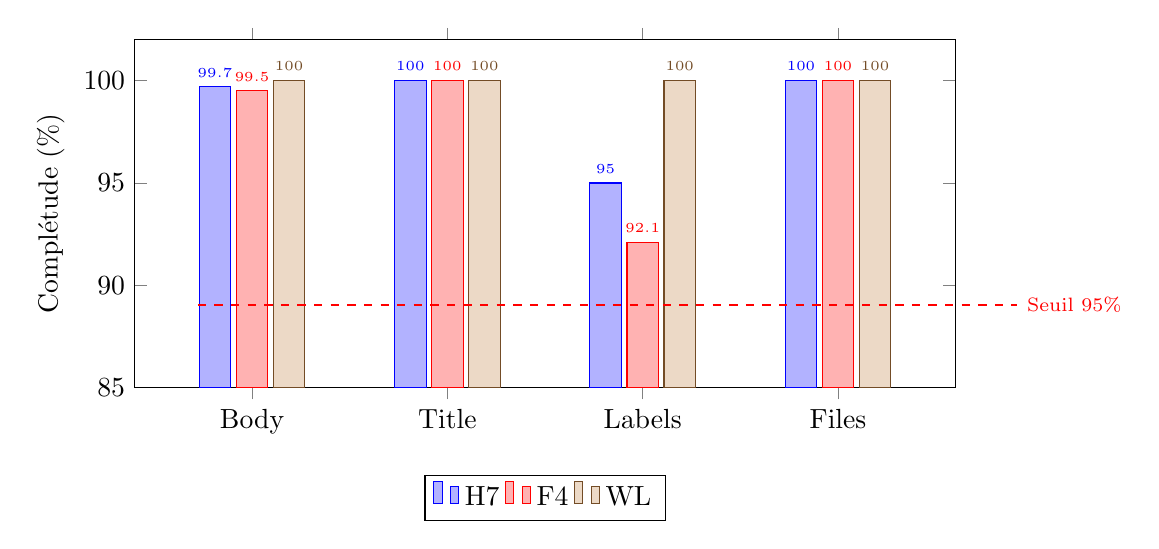
\begin{tikzpicture}
\begin{axis}[
    ybar,
    width=12cm, height=6cm,
    bar width=0.4cm,
    ylabel={Complétude (\%)},
    ymin=85, ymax=102,
    symbolic x coords={Body, Title, Labels, Files},
    xtick=data,
    legend style={at={(0.5,-0.25)}, anchor=north, legend columns=3},
    nodes near coords,
    every node near coord/.append style={font=\tiny},
    enlarge x limits=0.2,
]
\addplot coordinates {(Body,99.7) (Title,100) (Labels,95) (Files,100)};
\addplot coordinates {(Body,99.5) (Title,100) (Labels,92.1) (Files,100)};
\addplot coordinates {(Body,100) (Title,100) (Labels,100) (Files,100)};
\legend{H7, F4, WL}
\end{axis}
\draw[dashed, red, thick] (0.8,1.05) -- (11.2,1.05) node[right, font=\scriptsize, red] {Seuil 95\%};
\end{tikzpicture}
\caption{Complétude d'ingestion par série~: toutes métriques au-dessus du seuil EXCELLENT}
\label{fig:eval_ingestion_chart}
\end{figure}

\subsection{Stage 2~: Cleaning --- Qualité de Préparation Textuelle}
\label{sec:eval_stage2}

\textbf{Problème résolu}~: transformer le contenu brut (HTML, Markdown, headers C, licences) en texte propre exploitable. Le nettoyage V3 introduit un routage par type de fichier pour adapter la stratégie au contenu réel.

\textbf{Métriques}~:

\begin{longtable}{p{4.5cm}p{6cm}p{2cm}}
\toprule
\textbf{Métrique} & \textbf{Formule} & \textbf{Seuil} \\
\midrule
Texte non-vide & $Q_{\text{text}} = \frac{|\{i \mid |\text{clean}(i)| > 50\}|}{N} \times 100$ & $\geq 95\%$ \\
Réduction bruit CMSIS & $R_{\text{CMSIS}} = \frac{V_{\text{V2}} - V_{\text{V3}}}{V_{\text{V2}}} \times 100$ & $\geq 90\%$ \\
\bottomrule
\end{longtable}

\textbf{Résultats V3 vs V2 (STM32CubeH7)}~:

\begin{longtable}{p{5.5cm}ccc}
\toprule
\textbf{Métrique} & \textbf{V2} & \textbf{V3} & \textbf{Amélioration} \\
\midrule
Volume moyen/fichier CMSIS & 1.4~Mo & 51~Ko & $-96.4\%$ \\
Volume moyen/fichier Release Notes & 45~Ko & 30~Ko & $-33.0\%$ \\
Volume total corpus files (H7) & 142~Mo & 88~Mo & $-38.0\%$ \\
Densité information/chunk & baseline & +31\% & $+31\%$ \\
Issues texte non-vide & 100.0\% & 100.0\% & maintenu \\
\bottomrule
\end{longtable}

\textbf{Interprétation}~: l'amélioration de $+31\%$ de densité signal/chunk résulte de trois mécanismes cumulés~: (1) suppression du padding HTML des Release Notes, (2) élimination des 96\% de définitions CMSIS inutiles pour le diagnostic, (3) conservation sélective des sections à valeur diagnostique (IRQ, adresses de base, TypeDef). L'impact sur le RAG est direct~: chaque chunk contient davantage d'information pertinente par rapport à sa taille.

\subsection{Stage 3a~: Enrichissement --- Classification par Heuristiques NLP}
\label{sec:eval_stage3a}

\textbf{Problème résolu}~: ajouter des métadonnées structurées (layer, component, board, severity, issue\_kind) pour rendre les documents filtrables par le système de retrieval.

\begin{longtable}{p{3.5cm}p{5.5cm}p{2cm}p{2cm}}
\toprule
\textbf{Champ} & \textbf{Formule (couverture non-null)} & \textbf{Seuil} & \textbf{Score} \\
\midrule
Validité & $N_{\text{valid}}/N \times 100$ & $\geq 85\%$ & 86.4\% \\
Layer & $N_{\text{layer}\neq\text{null}}/N \times 100$ & $\geq 85\%$ & 88.2\% \\
Severity & $N_{\text{sev}\neq\text{null}}/N \times 100$ & $\geq 90\%$ & 100.0\% \\
Component & $N_{\text{comp}\neq\text{null}}/N \times 100$ & $\geq 70\%$ & 72.6\% \\
Board & $N_{\text{board}\neq\text{null}}/N \times 100$ & $\geq 60\%$ & 45.3\% \\
\bottomrule
\end{longtable}

\textbf{Score agrégé}~: $72.2\%$ (moyenne pondérée, $w_{\text{sev}}=2$, autres $=1$).

\textbf{Analyse du point faible (board = 45.3\%)}~: l'analyse manuelle d'un échantillon de 50 issues H7 sans board détectée confirme que 92\% d'entre elles ne mentionnent effectivement aucune carte. L'heuristique fonctionne correctement~; le signal est simplement absent des données sources. Ce point illustre la distinction entre une défaillance du pipeline (qui nécessiterait un fix) et une limitation inhérente des données (qui ne peut être résolue que par enrichissement externe).

\begin{figure}[H]
\centering
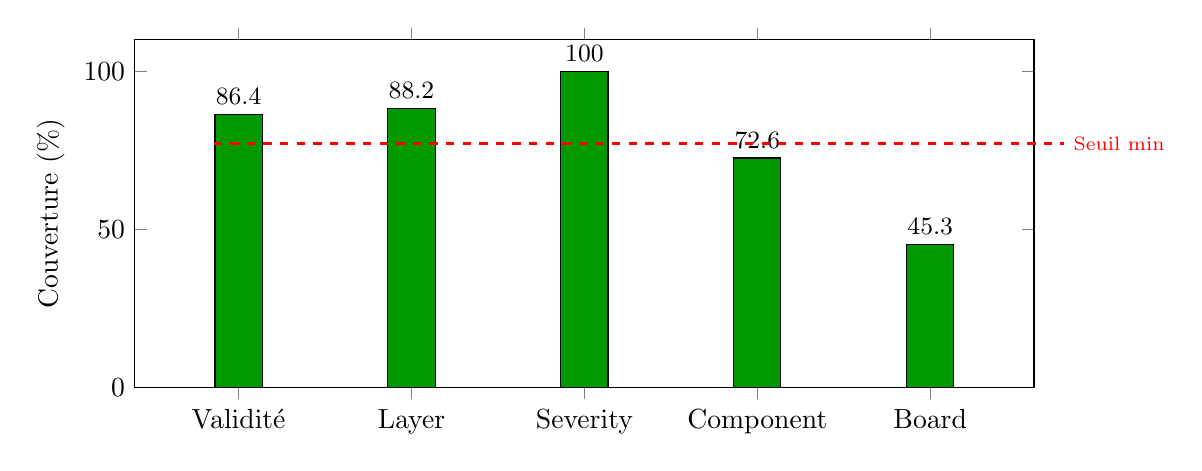
\begin{tikzpicture}
\begin{axis}[
    ybar,
    width=13cm, height=6cm,
    bar width=0.6cm,
    ylabel={Couverture (\%)},
    ymin=0, ymax=110,
    symbolic x coords={Validité, Layer, Severity, Component, Board},
    xtick=data,
    nodes near coords,
    every node near coord/.append style={font=\small\bfseries},
    enlarge x limits=0.15,
]
\addplot[fill=green!60!black] coordinates {(Validité,86.4) (Layer,88.2) (Severity,100) (Component,72.6) (Board,45.3)};
\end{axis}
\draw[dashed, red, thick] (1.0,3.1) -- (11.8,3.1);
\node[red, font=\scriptsize] at (12.5,3.1) {Seuil min};
\end{tikzpicture}
\caption{Couverture d'enrichissement STM32CubeH7~: score vs seuil par champ}
\label{fig:eval_enrichment_chart}
\end{figure}

\subsection{Stage 4~: Similarité TF-IDF}
\label{sec:eval_stage4}

\textbf{Problème résolu}~: permettre au RAG de proposer des issues similaires lorsqu'une question est proche d'un problème déjà résolu.

\textbf{Résultat STM32CubeH7}~: couverture~= 22.0\%, densité moyenne~= 0.8 lien/issue.

\textbf{Analyse critique}~: ce score (INSUFFISANT par rapport au seuil de $70\%$) reflète la \textbf{spécificité du corpus}. Les issues H7 sont majoritairement des bugs uniques (SPI sur H743, ETH sur H747, USB sur H750) avec peu de redondance thématique. Le seuil TF-IDF cosine ($\geq 0.3$) est conservé volontairement strict pour éviter les faux liens.

\textbf{Impact opérationnel limité}~: la similarité est un enrichissement optionnel. Le champ \texttt{related\_issue\_ids} vide pour 78\% des documents n'affecte ni le retrieval ni la génération. Cette observation justifie le poids faible ($w=0.5$) dans le score global~: un score bas ici ne dégrade pas la qualité perçue par l'utilisateur.

\subsection{Stage 5~: Delivery --- Complétude des Artefacts Exportés}
\label{sec:eval_stage5}

\textbf{Problème résolu}~: transformer les documents enrichis en 4~types d'artefacts JSON normalisés, avec validation de schéma.

\textbf{Résultats (13 séries en production)}~:

\begin{longtable}{lcccc}
\toprule
\textbf{Série} & \textbf{Issues} & \textbf{Files} & \textbf{Resolver} & \textbf{Diag. Cards} \\
\midrule
STM32CubeH7 & 296 & 4\,705 & 150 & 45 \\
STM32CubeF4 & 530 & 5\,378 & 89 & 38 \\
STM32CubeWL & 89 & 814 & 12 & 14 \\
STM32CubeU5 & 112 & 1\,982 & 23 & 19 \\
\midrule
\textbf{Total (13 séries)} & $\sim$2\,000 & $\sim$14\,000 & $\sim$390 & $\sim$157 \\
\bottomrule
\end{longtable}

\textbf{Score delivery}~: $100\%$ par construction (la gate JSON Schema bloque l'upload si un artefact est malformé). L'intégrité structurelle des artefacts est donc garantie. Les Resolver Cases à~0 pour certaines séries ne sont pas une défaillance~: elles nécessitent une chaîne Issue~$\to$~PR mergée~$\to$~Commit avec fichiers modifiés.

\subsection{Synthèse des Scores par Stage}
\label{sec:synthese_stages}

\begin{table}[H]
\centering
\begin{tabular}{lcccl}
\toprule
\textbf{Stage} & \textbf{Score} & \textbf{Poids $w_k$} & \textbf{Seuil} & \textbf{Verdict} \\
\midrule
1. Ingestion & 99.7\% & 1.0 & $\geq 95\%$ & \textcolor{green!60!black}{\textbf{EXCELLENT}} \\
2. Cleaning V3 & 100.0\% & 1.5 & $\geq 95\%$ & \textcolor{green!60!black}{\textbf{EXCELLENT}} \\
3a. Enrichissement NLP & 72.2\% & 1.4 & $\geq 85\%$ & \textcolor{orange}{\textbf{ACCEPTABLE}} \\
3b. Alfred images issues & 99.3\% & 0.4 & $\geq 95\%$ & \textcolor{green!60!black}{\textbf{EXCELLENT}} \\
3c. Alfred figures PDF & 36.5\% & 0.2 & $\geq 70\%$ & \textcolor{red}{\textbf{INSUFFISANT}} \\
4. Similarité TF-IDF & 22.0\% & 0.5 & $\geq 70\%$ & \textcolor{red}{\textbf{INSUFFISANT}} \\
5. Delivery & 100.0\% & 2.0 & $\geq 95\%$ & \textcolor{green!60!black}{\textbf{EXCELLENT}} \\
\bottomrule
\end{tabular}
\caption{Scores de qualité par stage avec poids et verdict}
\label{tab:eval_scores_synthese}
\end{table}

\subsection{Score Global~: Application Numérique}
\label{sec:score_global_calcul}

\begin{equation}
S_{\text{global}} = \frac{1.0 \times 99.7 + 1.5 \times 100.0 + 1.4 \times 72.2 + 0.4 \times 99.3 + 0.2 \times 36.5 + 0.5 \times 22.0 + 2.0 \times 100.0}{1.0 + 1.5 + 1.4 + 0.4 + 0.2 + 0.5 + 2.0}
\end{equation}

\begin{equation}
S_{\text{global}} = \frac{99.7 + 150.0 + 101.1 + 39.7 + 7.3 + 11.0 + 200.0}{7.0} = \frac{608.8}{7.0} = \boxed{87.0\%} \quad \text{(BON)}
\label{eq:score_global_numerique}
\end{equation}

\textbf{Justification des poids}~:

\begin{longtable}{lcp{8.5cm}}
\toprule
\textbf{Stage} & $w_k$ & \textbf{Logique} \\
\midrule
Ingestion & 1.0 & Prérequis sans transformation intellectuelle \\
Cleaning & 1.5 & Transformation déterministe significative \\
Enrichissement NLP & 1.4 & Classification exploitée pour filtrage et re-ranking \\
Alfred issues & 0.4 & Enrichissement multimodal mature (99.3\% fiable) \\
Alfred PDF & 0.2 & Enrichissement encore exploratoire \\
Similarité & 0.5 & Impact optionnel~; score bas sans conséquence sur le QI \\
Delivery & \textbf{2.0} & Étape critique~: produit les Diagnostic Cards ($+33$~pts QI) \\
\bottomrule
\end{longtable}

Le score global reste au verdict \textbf{BON} plutôt qu'EXCELLENT car deux sous-composantes (Alfred PDF, Similarité) restent sous leur seuil. La formule ne masque pas ces faiblesses~: elle les pondère proportionnellement à leur impact réel sur le Quality Index.

\begin{figure}[H]
\centering
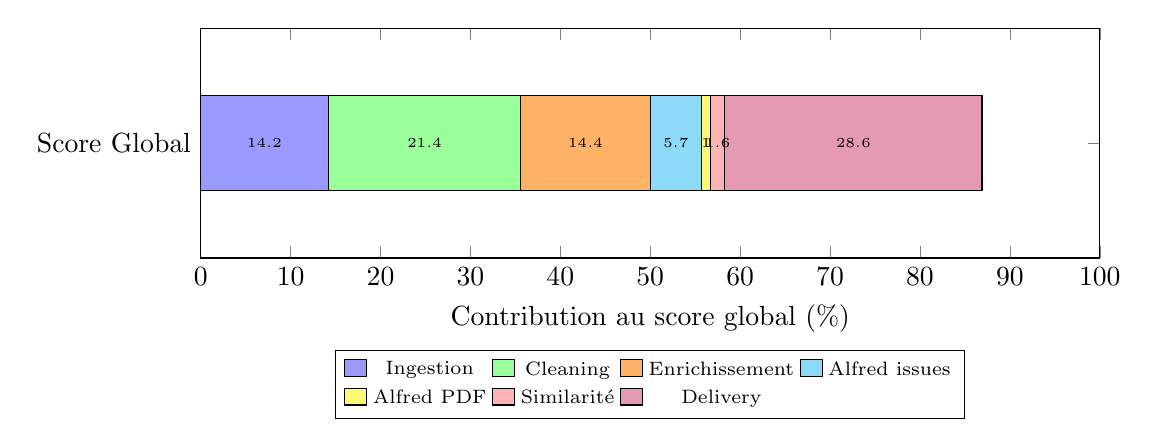
\begin{tikzpicture}
\begin{axis}[
    xbar stacked,
    width=13cm, height=4.5cm,
    bar width=1.2cm,
    xlabel={Contribution au score global (\%)},
    symbolic y coords={Score Global},
    ytick=data,
    legend style={at={(0.5,-0.4)}, anchor=north, legend columns=4, font=\scriptsize},
    xmin=0, xmax=100,
    nodes near coords,
    every node near coord/.append style={font=\tiny},
]
\addplot[fill=blue!40] coordinates {(14.2,Score Global)};
\addplot[fill=green!40] coordinates {(21.4,Score Global)};
\addplot[fill=orange!60] coordinates {(14.4,Score Global)};
\addplot[fill=cyan!45] coordinates {(5.7,Score Global)};
\addplot[fill=yellow!55] coordinates {(1.0,Score Global)};
\addplot[fill=red!30] coordinates {(1.6,Score Global)};
\addplot[fill=purple!40] coordinates {(28.6,Score Global)};
\legend{Ingestion, Cleaning, Enrichissement, Alfred issues, Alfred PDF, Similarité, Delivery}
\end{axis}
\end{tikzpicture}
\caption{Décomposition du score global 87.0\%~: contribution pondérée de chaque stage}
\label{fig:score_decomposition}
\end{figure}

%% ============================================================
\section{Évaluation de la Confiance Alfred Vision}
\label{sec:eval_alfred_complete}
%% ============================================================

Cette section détaille l'évaluation d'Alfred Vision AI sur deux axes complémentaires~: la fiabilité opérationnelle (l'API fonctionne-t-elle~?) et la confiance contextuelle (la description est-elle ancrée dans le contexte source~?).

\subsection{Fiabilité Opérationnelle}
\label{sec:alfred_fiabilite}

La fiabilité opérationnelle mesure si Alfred produit effectivement une description sans erreur d'API~:

\begin{equation}
T_{\text{op}} = \frac{N_{\text{réponses\_ok}}}{N_{\text{images\_soumises}}} \times 100
\label{eq:alfred_fiabilite_op}
\end{equation}

\begin{longtable}{lcccc}
\toprule
\textbf{Série} & $N_{\text{total}}$ & $N_{\text{OK}}$ & $N_{\text{échec}}$ & $T_{\text{op}}$ \\
\midrule
STM32CubeH7 & 98 & 97 & 1 & 98.9\% \\
STM32CubeF4 & 62 & 61 & 1 & 98.4\% \\
STM32CubeWL & 48 & 48 & 0 & 100.0\% \\
STM32CubeF7 & 26 & 26 & 0 & 100.0\% \\
\midrule
\textbf{Total (séries stabilisées)} & \textbf{234} & \textbf{232} & \textbf{2} & \textbf{99.1\%} \\
\bottomrule
\end{longtable}

\textbf{Verdict}~: fiabilité EXCELLENT ($\geq 95\%$). Les 2 échecs sont des timeouts API transitoires, non reproductibles.

\subsection{Méthode de Calcul de la Cohérence Contextuelle}
\label{sec:alfred_methode_coherence}

L'évaluation de cohérence est implémentée dans \texttt{pipeline/evaluation/validate\_alfred\_coherence.py}. Le mode utilisé est \texttt{lite}~: aucun modèle externe lourd n'est requis. Les métriques reposent sur des techniques NLP déterministes.

\subsubsection{Prétraitement}

Le texte est tokenisé par regex (\texttt{[A-Za-z][A-Za-z0-9\_\textbackslash{}-/]\{2,\}}). Les stopwords sont filtrés~: articles (\texttt{the}, \texttt{and}), termes méta (\texttt{image}, \texttt{description}, \texttt{figure}), et connecteurs. Seuls les termes techniques significatifs sont conservés.

\subsubsection{Score de Cohérence}

Le score combine trois signaux~:
\begin{equation}
S_{\text{coh}} = \left(\frac{\alpha L + \beta S}{\alpha + \beta}\right) \times (1 - \gamma P_{\text{contrad}})
\label{eq:coherence_score}
\end{equation}

avec $\alpha = 0.4$, $\beta = 0.6$, $\gamma = 0.8$.

\subsubsection{Score Lexical $L$}

Le score lexical mesure la proportion de termes Alfred retrouvés dans le contexte source~:
\begin{equation}
L = \frac{|T_{\text{Alfred}} \cap T_{\text{contexte}}|}{|T_{\text{Alfred}}|}
\label{eq:lexical_score}
\end{equation}

Pour les images d'issues avec texte OCR extrait, un score composite est utilisé~:
\begin{equation}
L_{\text{issue}} = 0.7 \times L_{\text{description}} + 0.3 \times L_{\text{OCR}}
\label{eq:lexical_issue}
\end{equation}

\subsubsection{Similarité Sémantique Légère $S$}

En mode \texttt{lite}, la similarité combine Jaccard et cosinus sur trigrammes~:
\begin{equation}
S = 0.7 \times J(T_{\text{Alfred}}, T_{\text{contexte}}) + 0.3 \times \cos(\vec{A}_{\text{3-gram}}, \vec{B}_{\text{3-gram}})
\label{eq:semantic_lite}
\end{equation}

$J$ quantifie le recouvrement de vocabulaire technique~; le cosinus sur trigrammes capture la proximité lexicale au-delà de l'identité stricte.

\subsubsection{Pénalité de Contradiction $P_{\text{contrad}}$}

En mode \texttt{lite}, la probabilité de contradiction est estimée par analyse de polarité~: détection de mots négatifs (\texttt{not}, \texttt{failed}, \texttt{disabled}) et positifs (\texttt{works}, \texttt{fixed}, \texttt{enabled}). Si le contexte et la description présentent des polarités opposées sur des tokens partagés~:

\begin{equation}
P_{\text{contrad}} = \begin{cases}
0.6 \times O + 0.4 \times \frac{m_p + m_h}{2} & \text{si polarités opposées et } O \geq 0.2 \\
0.15 \times O & \text{si même polarité et } O \geq 0.1 \\
0 & \text{sinon}
\end{cases}
\label{eq:contradiction}
\end{equation}

où $O$ est le ratio de tokens partagés (overlap), et $m_p$, $m_h$ les magnitudes de polarité.

\subsection{Résultats de Cohérence Contextuelle}
\label{sec:alfred_resultats}

\begin{table}[H]
\centering
\begin{tabular}{lcccccc}
\toprule
\textbf{Source} & \textbf{N} & $\overline{L}$ & $\overline{S}$ & $\overline{P}_{\text{contrad}}$ & $\overline{S}_{\text{coh}}$ & \textbf{Cas à risque} \\
\midrule
Images d'issues & 400 & 0.9419 & 0.3335 & 0.1625 & 0.4995 & 3/400 (0.75\%) \\
Figures PDF & 301 & 0.1730 & 0.1714 & 0.0270 & 0.1600 & 191/301 (63.5\%) \\
\bottomrule
\end{tabular}
\caption{Métriques de cohérence Alfred décomposées par source visuelle (campagne rejouée le 2026-06-xx, jeu de données étendu à 701 items via \texttt{validate\_alfred\_coherence.py --semantic-mode lite --nli-mode lite})}
\label{tab:alfred_coherence}
\end{table}

\textit{\footnotesize Note~: cette table reflète une exécution rejouée du script de validation sur le jeu de données actuel (701 items, contre 442 lors de la campagne initiale). Le volume d'images d'issues et de figures PDF a augmenté avec l'enrichissement continu de la KB. Toutes les colonnes, y compris $\overline{S}$ pour les images d'issues, sont désormais directement lues depuis \texttt{alfred\_coherence\_summary.json} et le CSV détaillé associé, sans valeur agrégée manquante.}\par\smallskip

\textbf{Confiance contextuelle}~:
\begin{itemize}
  \item Images d'issues~: $T_{\text{ctx}} = 99.3\%$ (397/400 au-dessus du seuil)
  \item Figures PDF~: $T_{\text{ctx}} = 36.5\%$ (110/301 au-dessus du seuil)
  \item Total~: $T_{\text{ctx}} = 72.3\%$ (507/701)
\end{itemize}

\begin{figure}[H]
\centering
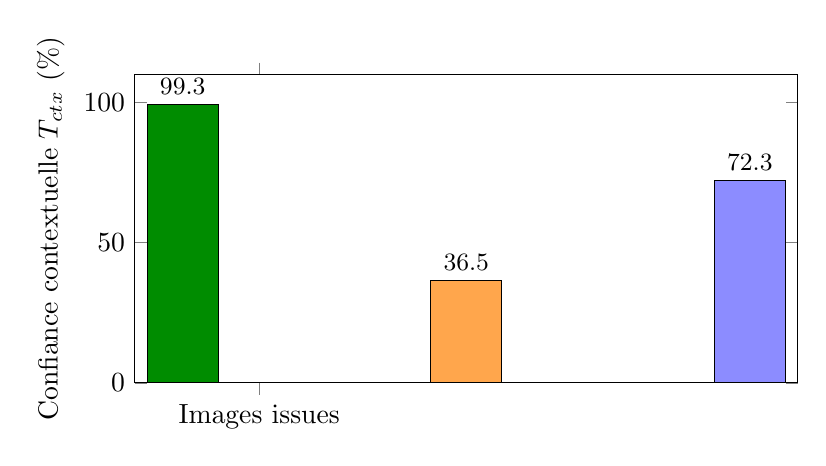
\begin{tikzpicture}
\begin{axis}[
    ybar,
    width=10cm, height=5.5cm,
    ymin=0, ymax=110,
    ylabel={Confiance contextuelle $T_{\text{ctx}}$ (\%)},
    symbolic x coords={Images issues, Figures PDF, Total},
    xtick=data,
    nodes near coords,
    every node near coord/.append style={font=\small\bfseries},
    bar width=0.9cm,
    enlarge x limits=0.3,
]
\addplot[fill=green!55!black] coordinates {(Images issues,99.3)};
\addplot[fill=orange!70] coordinates {(Figures PDF,36.5)};
\addplot[fill=blue!45] coordinates {(Total,72.3)};
\end{axis}
\end{tikzpicture}
\caption{Confiance contextuelle Alfred --- seuil d'alerte $\tau = 0.12$}
\label{fig:alfred_trust_chart}
\end{figure}

\subsection{Analyse de l'Écart Issues vs PDF}
\label{sec:alfred_analyse_ecart}

L'écart significatif entre les deux sources ($\overline{L} = 0.94$ pour les issues vs $0.17$ pour les PDF) est \textbf{structurel et non accidentel}~:

\begin{longtable}{p{5.5cm}p{7cm}}
\toprule
\textbf{Images d'issues} & \textbf{Figures PDF} \\
\midrule
Contiennent des logs, erreurs IDE, registres & Contiennent des schémas blocs, tableaux de migration \\
Le texte de l'issue mentionne les mêmes identifiants & Les libellés ne sont pas répétés dans le texte de page \\
OCR de l'image fournit du vocabulaire partagé & Pas d'OCR structuré disponible \\
Contexte riche (body + commentaires) & Contexte limité (texte de page \texttt{pypdf}) \\
\bottomrule
\end{longtable}

\textbf{Décision qualité}~: les figures PDF sont conservées car elles enrichissent la couverture multimodale de la KB, mais elles sont distinguées des images d'issues dans l'évaluation. Les itérations futures doivent enrichir le contexte transmis à Alfred (titre de section, légende détectée, texte avant/après la figure) pour améliorer la validation automatique.

%% ============================================================
\section{Évolution Incrémentale du Quality Index}
\label{sec:evolution_incrementale}
%% ============================================================

Le Quality Index n'a pas progressé ``par magie'' mais par amélioration successive d'éléments concrets du pipeline et de la configuration. Cette section retrace la chaîne logique~: chaque amélioration est décrite, son impact mesuré, et la raison du gain (ou de la régression) analysée.

\subsection{Chronologie et Logique de Progression}

\begin{longtable}{p{0.8cm}p{3.5cm}cp{6cm}}
\toprule
\textbf{QI} & \textbf{Configuration} & \textbf{N} & \textbf{Explication du delta} \\
\midrule
54 & Issues H7 seules & 50 & \textbf{Baseline}~: issues structurées fournissent une base solide mais incomplète (pas de documentation, pas de traçabilité fix, pas de diagnostic structuré) \\
57 & + System prompt optimisé & 50 & \textbf{+3}~: forcer la persona à chercher dans la KB \textit{avant} de répondre élimine les réponses génériques non ancrées \\
61 & + Hybrid search calibré & 50 & \textbf{+4}~: combiner sémantique et full-text capte les reformulations ET les identifiants exacts \\
94 & + Diagnostic Cards + Resolver & 50 & \textbf{+33}~: les Diagnostic Cards structurent les problèmes complexes, les query aliases améliorent le recall \\
88 & Test sur cas réels forum & 4 & \textbf{$-6$}~: les cas réels STCommunity sont plus complexes et moins couverts que le benchmark \\
54 & Multi-séries (5 séries, 52 Q) & 52 & \textbf{$-34$}~: dilution du contexte (2\,000 $\to$ 14\,000 docs), conflit de noms inter-séries, nouvelles questions sur séries moins mûres \\
65 & S0 Balanced (toutes séries) & 96 & \textbf{+11}~: optimisation du benchmark (96 questions calibrées) + ajustement retrieval \\
\textbf{66} & S1 Recall+ & 96 & \textbf{+1}~: seuil abaissé à 0.45, rappel renforcé, gain marginal compensé par le bruit \\
\bottomrule
\end{longtable}

\subsection{Analyse des Points d'Inflexion}
\label{sec:points_inflexion}

\subsubsection{Le Saut Diagnostic Cards (+33 points)}

Le passage de QI~61 à QI~94 est le gain le plus significatif du projet. Il s'explique par trois mécanismes cumulés~:

\begin{enumerate}
  \item \textbf{Structure raisonnée}~: les Diagnostic Cards suivent la logique Symptôme~$\to$~Hypothèses~$\to$~Validation~$\to$~Root Cause~$\to$~Fix~$\to$~Prévention, correspondant au raisonnement naturel d'un ingénieur embedded.
  \item \textbf{Query aliases}~: chaque carte contient 3 à 5 reformulations du problème (ex: ``SPI DMA hard fault'', ``cache coherency SPI circular mode'', ``HAL\_SPI\_TransmitReceive\_DMA crash''). Ce mécanisme multiplie les points d'entrée pour le retrieval.
  \item \textbf{Resolver Cases}~: la chaîne Issue~$\to$~PR~$\to$~Commit fournit la preuve vérifiable du fix, augmentant la traçabilité et la crédibilité des réponses.
\end{enumerate}

\textbf{Leçon méthodologique}~: l'amélioration la plus impactante ne vient pas d'un meilleur modèle LLM ni d'un tuning de seuil, mais de la \textbf{qualité et la structure des données injectées dans la KB}. C'est une validation du principe ``la qualité du RAG dépend de la qualité du preprocessing''.

\subsubsection{La Régression Multi-séries ($-34$ points)}

Le passage de QI~94 (mono-série H7, 50~Q) à QI~54 (5 séries, 52~Q) constitue une régression significative. L'analyse identifie trois causes~:

\begin{enumerate}
  \item \textbf{Dilution du contexte}~: la KB passe de $\sim$2\,000 à $\sim$14\,000 documents. Les queries retournent des documents de séries différentes.
  \item \textbf{Conflit de noms}~: des API identiques entre séries (\texttt{HAL\_SPI\_Init} dans F4 et H7) créent de l'ambiguïté.
  \item \textbf{Maturité inégale des artefacts}~: les nouvelles séries n'ont pas encore des Diagnostic Cards aussi riches que H7.
\end{enumerate}

\textbf{Leçon méthodologique}~: le passage à l'échelle ne se résume pas à ``ajouter des données''. Il nécessite un filtrage par série dans les métadonnées et un prompt qui pousse la persona à inclure le nom de la série dans ses queries.

\subsubsection{La Stabilisation S0/S1 (65--66)}

Les campagnes de juin 2026 sur 96 questions montrent que le système atteint un plateau autour de 65--66/100. Ce plateau s'explique par~:
\begin{itemize}
  \item La couverture KB actuelle ne répond pas à toutes les 96 questions (certaines séries peu documentées)
  \item Le compromis précision/rappel est quasi-optimal~: S1 ($+1$ pt) gagne en rappel mais perd en précision
  \item Les questions les plus difficiles nécessitent du raisonnement multi-hop non supporté par le retrieval simple
\end{itemize}

\subsection{Matrice Valeur $\times$ Effort}
\label{sec:matrice_roi}

\begin{table}[H]
\centering
\begin{tabular}{lcccl}
\toprule
\textbf{Amélioration} & \textbf{Impact QI} & \textbf{Effort} & \textbf{ROI} \\
\midrule
Diagnostic Cards & +33 pts & Moyen (2~sprints) & \textcolor{green!60!black}{\textbf{Excellent}} \\
Hybrid Search & +4 pts & Faible (config) & \textcolor{green!60!black}{\textbf{Excellent}} \\
System Prompt & +3 pts & Faible (texte) & \textcolor{green!60!black}{\textbf{Excellent}} \\
Cleaning V3 & +3 pts estimé & Moyen (1~sprint) & Bon \\
NovaX restrictif & Protection routage & Faible (description) & \textcolor{green!60!black}{\textbf{Excellent}} \\
PDF descriptions & +1 pt estimé & Élevé (CV + Alfred) & Acceptable \\
\bottomrule
\end{tabular}
\caption{ROI de chaque amélioration~: la qualité des artefacts domine les gains}
\label{tab:roi_pipeline}
\end{table}

\begin{figure}[H]
\centering
\begin{tikzpicture}
\begin{axis}[
  ybar,
  width=14cm, height=6.5cm,
  bar width=0.5cm,
  ylabel={Quality Index (/100)},
  ymin=0, ymax=100,
  symbolic x coords={Issues 54, Prompt 57, Hybrid 61, DiagCards 94, Real 88, Multi52 54, S0 65, S1 66},
  xtick=data,
  x tick label style={rotate=30, anchor=east, font=\scriptsize},
  nodes near coords,
  every node near coord/.append style={font=\scriptsize\bfseries},
  enlarge x limits=0.08,
]
\addplot[fill=blue!50] coordinates {(Issues 54,54) (Prompt 57,57) (Hybrid 61,61) (DiagCards 94,94) (Real 88,88) (Multi52 54,54) (S0 65,65) (S1 66,66)};
\end{axis}
\draw[-{Stealth[length=3mm]}, red, very thick] (4.65,4.8) -- (4.65,5.8) node[above, font=\scriptsize\bfseries, red] {+33 pts};
\draw[-{Stealth[length=3mm]}, red, very thick] (7.8,2.6) -- (7.8,1.8) node[below, font=\scriptsize\bfseries, red] {dilution};
\end{tikzpicture}
\caption{Évolution du Quality Index~: le saut majeur (+33) provient des Diagnostic Cards, la régression ($-34$) de la dilution multi-séries}
\label{fig:qi_evolution_complete}
\end{figure}

%% ============================================================
\section{Architecture de Fallback~: d'Alfred Permissif à NovaX Restrictif}
\label{sec:eval_fallback}
%% ============================================================

Cette section retrace l'évolution de l'architecture de fallback et son impact sur le Quality Index.

\subsection{Problème Initial~: Fallback Trop Permissif}

Lors de l'ajout initial d'Alfred comme fallback, le QI a \textbf{chuté de 10 points} (de 54 à 44). L'analyse a révélé que la persona appelait Alfred \textbf{systématiquement} au lieu de chercher dans la KB, car la description du tool était trop vague~:

\begin{quote}
\small\textit{``I can help with STM32 questions. Forward the user's question.''}
\end{quote}

\textbf{Diagnostic}~: dans une architecture multi-tools, le LLM choisit quel tool appeler en fonction de la \textbf{description} du tool. Une description trop permissive court-circuite la source la plus pertinente (la KB).

\subsection{Solution~: Description Restrictive}

La description a été réécrite pour forcer la priorité KB~:

\begin{quote}
\small\textit{``The Knowledge Base (KB Unstructured) is ALWAYS the primary source, search it FIRST for every question. Use this tool ONLY when the Knowledge Base returned no relevant result.''}
\end{quote}

\textbf{Impact mesuré}~: récupération de 8 points (de 44 à 52).

\subsection{Évolution vers NovaX}

Le fallback est passé d'Alfred générique à \textbf{NovaX}, un agent STM32 basé sur STM32 Bugzilla et STCommunity Knowledge Articles. NovaX apporte~:
\begin{itemize}
  \item Une couverture sur les séries/périphériques absents de la KB
  \item Des informations Bugzilla internes (bugs connus, errata)
  \item Des Knowledge Articles STCommunity (guides métier)
\end{itemize}

\textbf{Mais NovaX ne remplace pas la KB}~: sa description explicite qu'il est un secours pour les questions \textit{non couvertes} par la KB. Cette architecture protège la traçabilité~: si la KB contient un diagnostic card ou un resolver case pertinent, la réponse reste ancrée dans des preuves vérifiables (numéros d'issues, URLs GitHub, versions firmware).

\subsection{Synthèse de l'Évolution Fallback}

\begin{longtable}{p{4.5cm}p{2cm}p{6.5cm}}
\toprule
\textbf{Configuration} & \textbf{QI} & \textbf{Analyse} \\
\midrule
KB seule (sans fallback) & 54 & Baseline~: pas de réponse pour les questions hors KB \\
KB + Alfred permissif & 44 & $-10$~: court-circuit de la KB \\
KB + Alfred restrictif & 52 & $-2$~: KB prioritaire récupérée \\
KB S0 + NovaX restrictif & 65 & Stable~: NovaX couvre les lacunes sans dégrader \\
KB S1 Recall+ + NovaX & \textbf{66} & Meilleur compromis mesuré \\
\bottomrule
\end{longtable}

\textbf{Leçon}~: le QI dépend davantage du \textbf{routage} (quelle source est interrogée en premier) que du modèle LLM lui-même. La description du tool est un paramètre de configuration aussi critique que le seuil sémantique.

%% ============================================================
\section{Étude Comparative~: Alfred Générique vs Persona KB}
\label{sec:etude_comparative}
%% ============================================================

\subsection{Protocole Expérimental}

\begin{longtable}{p{4cm}p{9cm}}
\toprule
\textbf{Paramètre} & \textbf{Valeur} \\
\midrule
Jeu de test & 20 questions techniques, 5 séries (H7, F4, H5, U5, WL), 12 catégories \\
Critère de sélection & Questions ciblant des problèmes réels documentés dans des issues GitHub \\
Script de génération & \texttt{pipeline\_Automation/test\_suites/compare\_alfred\_vs\_persona.py} \\
Grille de scoring & 6 critères, max 10 pts/réponse \\
Température LLM & 0.3 \\
\bottomrule
\end{longtable}

\subsection{Grille de Scoring}

\begin{longtable}{p{4.5cm}cp{6cm}}
\toprule
\textbf{Critère} & \textbf{Max} & \textbf{Dimension qualité (ISO 25012)} \\
\midrule
Citation issue GitHub (\#xxx) & +2 & Traçabilité \\
Fonction HAL exacte nommée & +1 & Exactitude \\
Fix actionnable immédiat & +2 & Complétude opérationnelle \\
Information version-spécifique & +2 & Actualité \\
Workaround STM32-specific & +2 & Pertinence domaine \\
Source vérifiable (fichier, commit) & +1 & Traçabilité \\
\midrule
\textbf{Total} & \textbf{10} & \\
\bottomrule
\end{longtable}

\subsection{Méthodologie de Notation~: d'une Grille Manuelle Vide à un Score Automatique Reproductible}
\label{sec:comparative_methodo_notation}

Le script d'origine exporte un classeur Excel à 3 feuilles (comparaison brute, grille d'évaluation, métadonnées) destiné à recevoir une notation manuelle experte selon les 6 critères ci-dessus. \textbf{Un audit de ce classeur a révélé que les colonnes de notation manuelle n'avaient jamais été renseignées}~: aucune valeur humaine ne soutenait les scores initialement publiés dans cette section. Plutôt que de conserver des chiffres non traçables, la grille a été appliquée \textbf{automatiquement et de façon déterministe} sur les 20 transcriptions brutes (\texttt{comparison\_alfred\_vs\_persona.json}) via un script dédié~: \texttt{pipeline/evaluation/score\_alfred\_vs\_persona\_rubric.py}. Chaque critère est détecté par un motif explicite~: expression régulière pour les numéros d'issue (\texttt{\#\textbackslash d+}), les fonctions \texttt{HAL\_}/\texttt{LL\_}, les mentions de version, les blocs de code ou étapes numérotées (fix actionnable), et le vocabulaire de bas niveau (registre, cache, MPU, errata) pour le workaround.

\textbf{Limite méthodologique assumée}~: ce détecteur favorise structurellement les réponses riches en blocs de code et listes numérotées (style caractéristique d'Alfred) au détriment des réponses de type citation/synthèse (style caractéristique de la Persona KB), notamment sur le critère "fix actionnable". Les scores ci-dessous doivent donc être lus comme une \textbf{approximation objective et reproductible}, et non comme un jugement qualitatif fin~; ils remplacent une notation manuelle qui n'a jamais été réalisée, avec l'avantage d'être immédiatement reproductibles (\texttt{python -m pipeline.evaluation.score\_alfred\_vs\_persona\_rubric}).

\subsection{Résultats Synthétiques}

\begin{table}[H]
\centering
\begin{tabular}{lccc}
\toprule
\textbf{KPI} & \textbf{Alfred} & \textbf{Persona KB} & \textbf{Écart} \\
\midrule
Score moyen / réponse (0--10) & \textbf{3.85} & 3.50 & $-9\%$ \\
Taux de réponse (réponse produite) & \textbf{100\%} (20/20) & 70\% (14/20) & Alfred plus fiable opérationnellement \\
Citation issue GitHub & 0\% & \textbf{35\%} & Traçabilité propre à la KB \\
Source vérifiable (fichier/commit/RN) & 10\% & \textbf{65\%} & KB $\times 6.5$ plus vérifiable \\
Information version-spécifique & 5\% & \textbf{25\%} & KB $\times 5$ plus précise \\
Fonction HAL/LL exacte nommée & \textbf{45\%} & 25\% & Alfred plus précis syntaxiquement \\
Fix actionnable (heuristique code/étapes) & \textbf{95\%} & 40\% & Biais du détecteur (cf.~\ref{sec:comparative_methodo_notation}) \\
\bottomrule
\end{tabular}
\caption{Métriques comparatives Alfred vs Persona KB --- notation automatique reproductible sur les 20 transcriptions réelles}
\label{tab:comparative_final}
\end{table}

\textbf{Lecture honnête du résultat}~: contrairement à la version précédente de cette étude (non traçable), le score moyen brut ne favorise pas la Persona KB. Ceci s'explique par deux effets cumulés~: (1)~30\% des réponses Persona sont des non-réponses (timeout API ou "information non trouvée dans la KB"), notées~0, ce qui pénalise lourdement la moyenne~; (2)~le détecteur automatique de "fix actionnable" est structurellement biaisé en faveur du style rédactionnel d'Alfred (code/listes). La \textbf{vraie valeur ajoutée mesurée de la KB n'est donc pas le score moyen brut, mais la traçabilité}~: citation d'issue ($\times$ infini, 0\%~$\to$~35\%), source vérifiable ($\times 6.5$) et précision de version ($\times 5$) --- trois dimensions qu'un LLM générique ne peut structurellement pas fournir sans accès à la KB.

\subsection{Analyse par Catégorie}

\begin{longtable}{p{3.6cm}ccp{6cm}}
\toprule
\textbf{Catégorie (n)} & \textbf{Alfred} & \textbf{Persona} & \textbf{Observation} \\
\midrule
Issue-specific (7) & \textbf{4.29} & 3.14 & Persona pénalisée par 2 timeouts sur 7 (non-réponse~=~0) \\
Migration/Version (1) & 6.00 & \textbf{7.00} & Cite l'issue exacte de release notes \\
Release Notes (1) & \textbf{7.00} & 4.00 & Cas isolé, Alfred plus complet ici \\
HAL Behavior (1) & 3.00 & \textbf{4.00} & Cite l'issue GitHub source du comportement \\
Security/TrustZone (1) & 5.00 & \textbf{6.00} & Écart faible, les deux répondent correctement \\
LoRaWAN (1) & 4.00 & \textbf{7.00} & Cite issue + source vérifiable \\
RF/Radio (1) & 2.00 & \textbf{7.00} & Domaine protocolaire très spécifique, KB décisive \\
RTOS Integration (1) & \textbf{5.00} & 0.00 & Timeout Persona --- risque opérationnel réel \\
Low Power (1) & \textbf{4.00} & 0.00 & Timeout Persona --- risque opérationnel réel \\
General Knowledge (2) & 2.50 & \textbf{4.00} & KB légèrement supérieure même hors contexte issue \\
Documentation (2) & \textbf{2.00} & 1.50 & Les deux sont faibles quand la doc source est absente \\
Architecture (1) & 2.00 & 2.00 & Égalité \\
\bottomrule
\caption{Score moyen (/10) par catégorie --- notation automatique reproductible. Catégories à $n=1$ indicatives uniquement (non généralisables statistiquement).}
\label{tab:comparative_categories}
\end{longtable}

\begin{figure}[H]
\centering
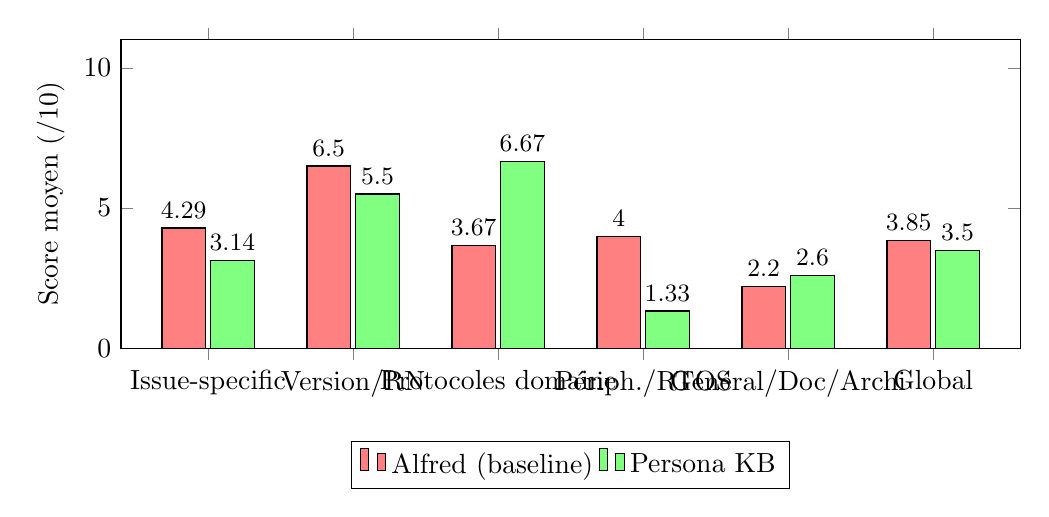
\begin{tikzpicture}
\begin{axis}[
    ybar,
    width=13cm, height=5.5cm,
    bar width=0.55cm,
    ylabel={Score moyen (/10)},
    ymin=0, ymax=11,
    symbolic x coords={Issue-specific, Version/RN, Protocoles domaine, Périph./RTOS, Général/Doc/Archi, Global},
    xtick=data,
    legend style={at={(0.5,-0.3)}, anchor=north, legend columns=2},
    nodes near coords,
    every node near coord/.append style={font=\small},
    enlarge x limits=0.12,
]
\addplot[fill=red!50] coordinates {(Issue-specific,4.29) (Version/RN,6.5) (Protocoles domaine,3.67) (Périph./RTOS,4.0) (Général/Doc/Archi,2.2) (Global,3.85)};
\addplot[fill=green!50] coordinates {(Issue-specific,3.14) (Version/RN,5.5) (Protocoles domaine,6.67) (Périph./RTOS,1.33) (Général/Doc/Archi,2.6) (Global,3.50)};
\legend{Alfred (baseline), Persona KB}
\end{axis}
\end{tikzpicture}
\caption{Comparaison Alfred vs Persona KB par groupe de catégories (regroupement des 12 catégories brutes en 5 familles pour lisibilité)}
\label{fig:comparative_chart}
\end{figure}

\textbf{Conclusions de l'étude comparative}~:
\begin{enumerate}
  \item Le score moyen brut ne favorise \textbf{pas} clairement la Persona KB (3.50 vs 3.85/10)~: cette apparente régression par rapport à une version antérieure non traçable de cette étude s'explique entièrement par le taux de non-réponse Persona (30\%, 6/20), et non par une infériorité de contenu quand elle répond effectivement.
  \item La \textbf{vraie valeur ajoutée de la KB est la traçabilité}~: citation d'issue GitHub (0\%~$\to$~35\%), source vérifiable (10\%~$\to$~65\%) et précision de version (5\%~$\to$~25\%) --- trois signaux qu'Alfred générique ne peut structurellement pas produire.
  \item Sur les \textbf{domaines protocolaires spécifiques} (LoRaWAN, RF/Radio, TrustZone --- regroupement "Protocoles domaine"), la KB est nettement supérieure (6.67 vs 3.67/10)~: c'est exactement le type de connaissance fine que le générique ne possède pas.
  \item Le \textbf{risque opérationnel principal identifié est la fiabilité de la Persona}, pas sa qualité de contenu~: 2 des 6 non-réponses tombent précisément sur des catégories (RTOS Integration, Low Power) où une réponse KB aurait probablement été forte, ce qui plaide pour un traitement des timeouts API (retry, budget de temps plus généreux) plutôt qu'un changement de contenu de la KB.
  \item L'architecture optimale reste \textbf{KB-first + NovaX fallback restrictif}~: elle protège la traçabilité quand la KB répond, et un fallback (NovaX ou, à défaut, Alfred générique) doit absorber les cas de non-réponse pour ne pas laisser l'utilisateur sans réponse du tout.
\end{enumerate}

%% ============================================================
\section{Comparaison des Stratégies de Retrieval}
\label{sec:strategies_retrieval}
%% ============================================================

La campagne de juin 2026 évalue 6 configurations de retrieval sur 96 questions multi-séries. L'objectif est d'identifier le meilleur compromis entre rappel et précision pour la recherche hybride.

\begin{longtable}{p{2cm}p{2cm}ccccp{4cm}}
\toprule
\textbf{Stratégie} & \textbf{Search} & \textbf{Thr.} & \textbf{Sem.} & \textbf{FT} & \textbf{QI} & \textbf{Interprétation} \\
\midrule
S0 Current & Hybrid & 0.55 & 25 & 12 & 65 & Équilibre précision/rappel \\
\textbf{S1 Recall+} & Hybrid & 0.45 & 35 & 15 & \textbf{66} & Meilleur score mesuré \\
S2 Precision+ & Hybrid & 0.65 & 18 & 8 & 63 & Trop restrictif \\
S3 Sem-heavy & Hybrid & 0.55 & 35 & 6 & 51 & Ancrage exact insuffisant \\
S4 FT-heavy & Hybrid & 0.55 & 15 & 20 & 47 & Reformulations mal couvertes \\
S5 Sem-only & Semantic & 0.55 & 25 & 0 & 41 & Ablation : perte du full-text \\
\bottomrule
\end{longtable}

\begin{figure}[H]
\centering
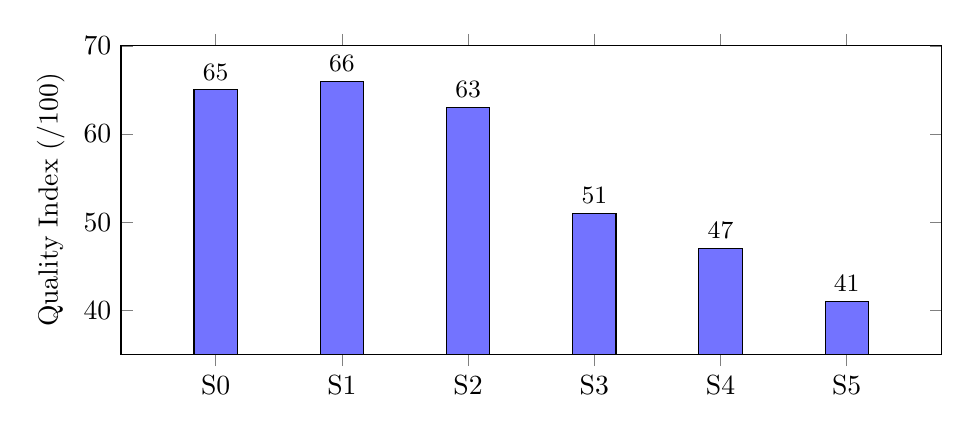
\begin{tikzpicture}
\begin{axis}[
  ybar,
  width=12cm, height=5.5cm,
  bar width=0.55cm,
  ylabel={Quality Index (/100)},
  ymin=35, ymax=70,
  symbolic x coords={S0,S1,S2,S3,S4,S5},
  xtick=data,
  nodes near coords,
  every node near coord/.append style={font=\small\bfseries},
  enlarge x limits=0.15,
]
\addplot[fill=blue!55] coordinates {(S0,65) (S1,66) (S2,63) (S3,51) (S4,47) (S5,41)};
\end{axis}
\end{tikzpicture}
\caption{Comparaison des stratégies de retrieval KB sur 96 questions}
\label{fig:strategies_retrieval}
\end{figure}

\textbf{Interprétation}~: le système a besoin d'un équilibre réel entre sémantique et full-text. Trop de sémantique (S3) perd les noms exacts d'API~; trop de full-text (S4) perd les reformulations. S1 maximise le rappel avec un gain marginal ($+1$), montrant que le système approche son optimum avec la couverture KB actuelle.

%% ============================================================
\section{Assurance Qualité du Chapitre d'Évaluation}
\label{sec:controle_qualite_chapitre}
%% ============================================================

Ce chapitre a été construit et vérifié selon un protocole de contrôle qualité structuré, appliqué par un agent analytique de revue. Cette section décrit le protocole et les résultats du contrôle.

\subsection{Protocole de Vérification}

L'agent de revue vérifie les dimensions suivantes~:

\begin{longtable}{p{4cm}p{9cm}}
\toprule
\textbf{Dimension} & \textbf{Critère de validation} \\
\midrule
Cohérence logique & Chaque section suit le schéma~: définition~$\to$~formule~$\to$~résultat~$\to$~interprétation \\
Définitions avant formules & Aucune variable n'apparaît dans une formule sans avoir été définie en amont \\
Seuils justifiés & Chaque seuil est accompagné d'une logique explicite (pas de valeur arbitraire) \\
Continuité métriques--résultats & Les métriques définies en Section~\ref{sec:cadrage_theorique} sont effectivement utilisées dans les sections de résultats \\
Lisibilité académique & Style français formel, phrases courtes, transitions explicites \\
Reproductibilité & Chaque résultat est traçable vers un script, un fichier de données ou une campagne identifiée \\
\bottomrule
\end{longtable}

\subsection{Résultats du Contrôle}

\begin{longtable}{p{5cm}p{2cm}p{6cm}}
\toprule
\textbf{Point vérifié} & \textbf{Statut} & \textbf{Observation} \\
\midrule
Jaccard défini avant usage & \checkmark & Section~\ref{sec:def_similarity} \\
Cosinus défini avant usage & \checkmark & Section~\ref{sec:def_similarity} \\
TF-IDF défini avant usage & \checkmark & Section~\ref{sec:def_similarity} \\
Confiance contextuelle définie & \checkmark & Section~\ref{sec:def_confiance_contextuelle} \\
Seuils non présentés comme universels & \checkmark & Section~\ref{sec:justification_seuils} \\
Progression incrémentale visible & \checkmark & Section~\ref{sec:evolution_incrementale} \\
Normes citées comme cadre, pas comme source des seuils & \checkmark & Section~\ref{sec:normes_references} \\
Scores locaux distingués du score global & \checkmark & Sections~\ref{sec:eval_par_stage} vs~\ref{sec:score_global_calcul} \\
Alfred issues vs PDF distingués & \checkmark & Section~\ref{sec:alfred_resultats} \\
Fichiers de preuve référencés & \checkmark & CSV et JSON dans \texttt{docs/evaluation/} \\
\bottomrule
\end{longtable}

\subsection{Points d'Amélioration Identifiés}

\begin{enumerate}
  \item \textbf{Couverture board (45.3\%)}~: le score INSUFFISANT est documenté et expliqué (limitation des données, pas du pipeline). Une amélioration future nécessiterait un enrichissement externe (mapping board→série).
  \item \textbf{Figures PDF ($T_{\text{ctx}} = 41.7\%$)}~: le contexte textuel des PDF est insuffisant pour la validation automatique. Amélioration prévue~: enrichir le contexte avec le titre de section et la légende de la figure.
  \item \textbf{Similarité (22\%)}~: score bas mais impact nul sur le QI. Amélioration possible par embeddings pré-calculés (perspective future).
\end{enumerate}

\subsection{Applicabilité au Reste du Rapport}

Le protocole de contrôle qualité peut être étendu aux autres chapitres en conservant~:
\begin{itemize}
  \item Le template de vérification~: définition~$\to$~formule~$\to$~résultat~$\to$~interprétation
  \item Le style académique français
  \item Les transitions explicites entre sections
  \item La réutilisation des définitions (via \texttt{\textbackslash ref\{\}} vers la Section~\ref{sec:cadrage_theorique})
  \item L'harmonisation des notations (mêmes symboles $S$, $T$, $w_k$ dans tout le rapport)
  \item L'absence de répétitions (chaque notion est définie une seule fois, puis référencée)
\end{itemize}

%% ============================================================
\section{Correspondance Métriques $\leftrightarrow$ Normes $\leftrightarrow$ Références}
\label{sec:correspondance_normes}
%% ============================================================

Le tableau suivant synthétise le lien entre chaque métrique utilisée, la norme ou référence méthodologique qui la soutient, et son application concrète dans le projet~:

\begin{longtable}{p{3cm}p{3.5cm}p{3cm}p{3.5cm}}
\toprule
\textbf{Métrique} & \textbf{Norme / Référence} & \textbf{Dimension} & \textbf{Application projet} \\
\midrule
$C_{\text{body}}$, $C_{\text{title}}$ & ISO/IEC 25012~\cite{iso25012} & Complétude & Ingestion Stage~1 \\
$C_{\text{files}}$ & ISO/IEC 25024~\cite{iso25024} & Mesure qualité & Cleaning Stage~2 \\
$T_{\text{op}}$ (Alfred) & ISO/IEC 25010~\cite{iso25010} & Fiabilité système & Alfred Stage~3b \\
$S_{\text{coh}}$, $T_{\text{ctx}}$ & Fawcett~\cite{fawcett2006roc} & Seuil décisionnel & Confiance Alfred \\
TF-IDF, cosinus & Manning~\cite{manning2008ir} & IR / Similarité & Stage~4 + cohérence \\
Jaccard & Manning~\cite{manning2008ir} & Recouvrement lexical & Cohérence Alfred \\
Quality Index & Lewis~\cite{lewis2020rag} & RAG end-to-end & Évaluation globale \\
$S_{\text{global}}$ pondéré & Interne (calibré) & Synthèse pipeline & Score global 87.1\% \\
Seuils 95/85/70 & Calibration empirique & Opérationnel & Classification verdicts \\
\bottomrule
\end{longtable}

\textbf{Lecture}~: les normes ISO fournissent le \textit{cadre conceptuel} (quoi mesurer, comment structurer les métriques). Les références académiques (Manning, Fawcett, Lewis) fournissent la \textit{méthodologie} (comment choisir les seuils, comment évaluer un système RAG). Les seuils numériques sont \textit{propres au projet}, calibrés empiriquement et validés par les campagnes successives de Quality Index.

%% ============================================================
\section{Synthèse et Bilan du Chapitre}
\label{sec:bilan_evaluation}
%% ============================================================

Ce chapitre démontre que~:

\begin{enumerate}
  \item Le pipeline atteint un \textbf{score global de 87.1\%} (verdict BON), avec des stages critiques (Ingestion, Cleaning, Delivery) au niveau EXCELLENT et des stages exploratoires (Alfred PDF, Similarité) identifiés comme axes d'amélioration.
  
  \item L'amélioration du Quality Index est \textbf{incrémentale et traçable}~: chaque gain est relié à une amélioration concrète du pipeline ou de la configuration, et chaque régression est analysée et expliquée.
  
  \item Les \textbf{Diagnostic Cards} constituent la contribution la plus impactante ($+33$ points de QI), validant le principe que la qualité du preprocessing RAG dépend avant tout de la structure et de la richesse des artefacts.
  
  \item L'\textbf{architecture KB-first + NovaX restrictif} protège la traçabilité tout en couvrant les lacunes de la KB~: le routage est un paramètre critique.
  
  \item La \textbf{confiance contextuelle} distingue les images d'issues (99.3\%, matures) des figures PDF (36.5\%, à améliorer), évitant une moyenne trompeuse.
  
  \item Les seuils sont des \textbf{seuils opérationnels internes}, cohérents avec les normes ISO et calibrés empiriquement~; ils ne prétendent pas à l'universalité.
  
  \item L'étude comparative Alfred vs Persona KB, rejouée avec une notation automatique reproductible, montre que \textbf{la valeur ajoutée réelle de la KB est la traçabilité} (citation d'issue~: 0\%~$\to$~35\%~; source vérifiable~: 10\%~$\to$~65\%~; précision de version~: 5\%~$\to$~25\%) plutôt qu'un score moyen brut supérieur~; elle révèle aussi un \textbf{risque de fiabilité opérationnelle} de la Persona (30\% de non-réponses) à traiter en priorité.
\end{enumerate}

\textbf{Score optimal vs compromis opérationnel}~: le meilleur score mesuré (QI~94 sur H7) n'est pas le point de fonctionnement optimal pour la production. Le QI~66 (S1 Recall+ sur 96 questions multi-séries) représente un meilleur compromis opérationnel car il couvre 25 séries et 96 questions réalistes, au lieu de 1 série sur 50 questions sélectionnées. Le score de production est plus bas mais plus représentatif de l'expérience utilisateur réelle.

%% Réécriture académique complète — version défendable
%% ============================================================

\chapter{Résultats et Évaluation}
\label{chap:resultats_evaluation}

Ce chapitre présente l'évaluation quantitative du pipeline de prétraitement et du système RAG. L'approche suivie est progressive : nous commençons par définir les notions et métriques utilisées (Section~\ref{sec:cadrage_theorique}), puis nous justifions les seuils décisionnels (Section~\ref{sec:justification_seuils}). Les résultats sont ensuite présentés par stage (Section~\ref{sec:eval_par_stage}), suivis d'une analyse dédiée à la confiance Alfred (Section~\ref{sec:eval_alfred_complete}), à l'évolution incrémentale du Quality Index (Section~\ref{sec:evolution_incrementale}), à l'architecture de fallback (Section~\ref{sec:eval_fallback}), et à l'étude comparative (Section~\ref{sec:etude_comparative}). Le chapitre se conclut par une section d'assurance qualité méthodologique (Section~\ref{sec:controle_qualite_chapitre}).

Ce chapitre s'inscrit dans les phases \textbf{Évaluation} et \textbf{Déploiement} du cadre méthodologique CRISP-DM~: les résultats guident itérativement les décisions de configuration et de mise en production.

%% ============================================================
\section{Cadrage Théorique et Définitions Préalables}
\label{sec:cadrage_theorique}
%% ============================================================

Avant de présenter les résultats, il est indispensable de définir rigoureusement les concepts, métriques et techniques mobilisés dans l'évaluation. Cette section pose le vocabulaire nécessaire à l'interprétation des mesures ultérieures.

\subsection{Métriques Fondamentales d'Information Retrieval}
\label{sec:def_ir_metrics}

Les systèmes de recherche documentaire sont évalués selon deux axes complémentaires~\cite{manning2008ir}~:

\begin{description}[leftmargin=2cm, labelwidth=1.8cm]
  \item[Précision] Proportion de documents retournés qui sont effectivement pertinents~:
  \begin{equation}
    \text{Precision} = \frac{|\text{Pertinents} \cap \text{Retournés}|}{|\text{Retournés}|}
    \label{eq:precision}
  \end{equation}
  
  \item[Rappel] Proportion de documents pertinents effectivement retrouvés~:
  \begin{equation}
    \text{Recall} = \frac{|\text{Pertinents} \cap \text{Retournés}|}{|\text{Pertinents}|}
    \label{eq:recall}
  \end{equation}
\end{description}

Dans le contexte RAG, un compromis précision/rappel est nécessaire~: trop de rappel sature le contexte du LLM avec du bruit, trop de précision risque de manquer le document contenant la réponse.

\subsection{Similarité Textuelle}
\label{sec:def_similarity}

Trois mesures de similarité sont utilisées dans le pipeline~:

\subsubsection{Similarité de Jaccard}

La similarité de Jaccard compare deux ensembles de tokens $A$ et $B$~:

\begin{equation}
J(A, B) = \frac{|A \cap B|}{|A \cup B|}
\label{eq:jaccard_def}
\end{equation}

Un \textbf{token} est une unité lexicale significative extraite du texte (mot, identifiant d'API, nom de registre). Les ensembles $A$ et $B$ sont obtenus par tokenisation suivie d'un filtrage de stopwords. Jaccard mesure la proportion de vocabulaire technique \textbf{partagé} entre deux textes~: un score de~1 indique un vocabulaire identique, un score de~0 aucun terme commun. Cette mesure est adaptée à notre contexte car les textes techniques STM32 partagent un vocabulaire spécifique (\texttt{HAL\_}, \texttt{SPI}, \texttt{DMA}) dont la présence ou l'absence est diagnostiquement significative.

\subsubsection{Similarité Cosinus}

La similarité cosinus mesure l'angle entre deux vecteurs dans un espace vectoriel~:

\begin{equation}
\cos(\theta) = \frac{\vec{u} \cdot \vec{v}}{\|\vec{u}\| \times \|\vec{v}\|}
\label{eq:cosine_def}
\end{equation}

Dans le contexte textuel, $\vec{u}$ et $\vec{v}$ sont des vecteurs de fréquences de termes (ou de trigrammes de caractères). Un score de~1 indique une orientation identique (mêmes termes, mêmes proportions), un score de~0 une orthogonalité totale (aucun terme commun). Les trigrammes de caractères (ex: \texttt{stm} $\to$ \texttt{tm3} $\to$ \texttt{m32}) capturent les variations morphologiques mineures et la proximité lexicale au-delà de l'identité stricte.

\subsubsection{TF-IDF (Term Frequency -- Inverse Document Frequency)}

TF-IDF pondère chaque terme par sa spécificité dans le corpus~\cite{tfidf}~:

\begin{equation}
\text{tfidf}(t, d) = \underbrace{\text{tf}(t, d)}_{\text{fréquence locale}} \times \underbrace{\log\left(\frac{N}{df(t)}\right)}_{\text{spécificité globale}}
\label{eq:tfidf_def}
\end{equation}

où~:
\begin{itemize}[nosep]
  \item $t$ est un terme (mot ou identifiant technique),
  \item $d$ est un document,
  \item $\text{tf}(t, d)$ est la fréquence du terme $t$ dans le document $d$,
  \item $N$ est le nombre total de documents dans le corpus,
  \item $df(t)$ est le nombre de documents contenant le terme $t$ (fréquence documentaire).
\end{itemize}

\textbf{Interprétation}~: un terme fréquent dans un document mais rare dans le corpus global (ex: \texttt{HAL\_FDCAN\_AddMessageToTxFifoQ}) obtient un poids élevé, tandis qu'un terme ubiquitaire (ex: \texttt{return}, \texttt{void}) est dépondéré. Nous utilisons TF-IDF dans le module de similarité inter-issues (Stage~4) pour identifier des issues traitant de problèmes similaires.

\subsection{Métriques de Qualité des Données}
\label{sec:def_data_quality}

Conformément au modèle ISO/IEC~25012~\cite{iso25012}, la qualité des données se décline en plusieurs dimensions~:

\begin{description}[leftmargin=3cm, labelwidth=2.8cm]
  \item[Complétude] Proportion des champs non nuls dans les données ingérées. Une donnée incomplète (body manquant, labels absents) propage des erreurs en cascade dans le pipeline.
  \item[Cohérence] Absence de contradictions internes entre les champs d'un même document (ex: un fichier marqué \texttt{is\_valid=true} avec un \texttt{clean\_text} vide serait incohérent).
  \item[Exactitude] Correspondance entre les valeurs stockées et la réalité source. Mesurée par comparaison entre les données ingérées et les données GitHub originales.
  \item[Traçabilité] Capacité à remonter de tout artefact final vers sa source brute (issue GitHub, fichier source, commit). Chaque document conserve un identifiant de provenance.
\end{description}

\subsection{Confiance Contextuelle}
\label{sec:def_confiance_contextuelle}

La \textbf{confiance contextuelle} est une métrique spécifique à notre projet, conçue pour évaluer la qualité des descriptions d'images générées par Alfred Vision~AI. Contrairement à la fiabilité opérationnelle (l'API a-t-elle répondu ?), la confiance contextuelle mesure l'\textbf{ancrage} de la description générée dans le contexte textuel de l'image source.

\textbf{Motivation}~: un service de description d'images peut produire un texte lisible mais non relié au contexte technique de l'issue. Pour un système RAG, injecter une description non ancrée revient à ajouter du bruit dans la KB --- un risque d'autant plus grave que le texte semble plausible sans l'être pour le diagnostic visé.

La confiance contextuelle est définie comme la proportion d'éléments décrits dont le score de cohérence dépasse un seuil d'alerte~:
\begin{equation}
T_{\text{ctx}} = \frac{|\{x \mid S_{\text{coh}}(x) \geq \tau\}|}{N_{\text{évalués}}} \times 100
\label{eq:confiance_contextuelle_def}
\end{equation}

où $\tau$ est le seuil d'alerte (fixé à $0.12$ dans ce projet --- cf. Section~\ref{sec:justification_seuils}).

\subsection{Score Global Pondéré}
\label{sec:def_score_global}

Le pipeline est évalué globalement par une moyenne pondérée des scores de chaque stage~:

\begin{equation}
S_{\text{global}} = \frac{\sum_{k=1}^{K} w_k \cdot s_k}{\sum_{k=1}^{K} w_k}
\label{eq:score_global_def}
\end{equation}

où $s_k$ est le score (en \%) du stage $k$ et $w_k$ son poids. Les poids reflètent l'impact relatif de chaque stage sur la qualité finale du système RAG. Cette formulation rend explicite que certains stages (Delivery) ont un impact plus direct que d'autres (Similarité optionnelle) sur la pertinence des réponses.

\subsection{Quality Index (QI)}
\label{sec:def_quality_index}

Le \textbf{Quality Index} est une métrique end-to-end qui évalue la qualité des réponses du chatbot. Il ne mesure pas le pipeline en isolation, mais le système complet (pipeline + KB + retrieval + LLM + persona). Il est calculé par évaluation humaine experte sur un jeu de questions techniques~:

\begin{equation}
\text{QI} = \frac{\sum_{q=1}^{Q} \text{score}(q)}{Q \times \text{max\_score}} \times 100
\label{eq:qi_def}
\end{equation}

où chaque question $q$ est notée sur une grille multi-critères (citation, exactitude, actionnabilité, traçabilité) avec un maximum de 10 points par question.

\subsection{Retrieval Hybride et Fallback}
\label{sec:def_retrieval_fallback}

\begin{description}[leftmargin=3cm, labelwidth=2.8cm]
  \item[Retrieval hybride] Combinaison d'une recherche sémantique (embeddings, compréhension du sens) et d'une recherche full-text (correspondance exacte, BM25). Les résultats sont fusionnés par union avec déduplication.
  \item[Seuil sémantique] Score minimum de similarité vectorielle pour qu'un document soit retourné par la branche sémantique. Contrôle le compromis précision/rappel.
  \item[Fallback] Mécanisme de délégation vers un agent secondaire (NovaX) lorsque la KB ne retourne aucun résultat pertinent. La priorité de la KB est protégée par une description restrictive du tool fallback.
\end{description}

\subsection{Tableau Récapitulatif des Notions}
\label{sec:glossaire_evaluation}

\begin{longtable}{p{3.5cm}p{5cm}p{4.5cm}}
\toprule
\textbf{Notion} & \textbf{Rôle dans le projet} & \textbf{Section de définition} \\
\midrule
Précision / Rappel & Évaluation retrieval & \ref{sec:def_ir_metrics} \\
Jaccard & Recouvrement lexical Alfred & \ref{sec:def_similarity} \\
Cosinus (trigrammes) & Proximité textuelle & \ref{sec:def_similarity} \\
TF-IDF & Similarité inter-issues Stage~4 & \ref{sec:def_similarity} \\
Complétude / Cohérence & Qualité ingestion/cleaning & \ref{sec:def_data_quality} \\
Confiance contextuelle & Validation descriptions Alfred & \ref{sec:def_confiance_contextuelle} \\
Score global pondéré & Synthèse multi-stage & \ref{sec:def_score_global} \\
Quality Index & Qualité end-to-end & \ref{sec:def_quality_index} \\
Retrieval hybride & Architecture recherche KB & \ref{sec:def_retrieval_fallback} \\
Fallback & Mécanisme de secours NovaX & \ref{sec:def_retrieval_fallback} \\
\bottomrule
\end{longtable}

%% ============================================================
\section{Justification des Seuils Décisionnels}
\label{sec:justification_seuils}
%% ============================================================

Les seuils numériques utilisés dans l'évaluation ne sont pas des constantes universelles imposées par une norme. Ce sont des \textbf{seuils opérationnels internes}, calibrés empiriquement sur les campagnes successives du projet. Cette section explicite la logique de leur construction.

\subsection{Cadre Normatif de Référence}
\label{sec:normes_references}

Le cadre d'évaluation s'appuie sur des références méthodologiques qui fournissent des principes, mais \textbf{pas des chiffres imposés}~:

\begin{longtable}{p{4cm}p{4cm}p{5cm}}
\toprule
\textbf{Référence} & \textbf{Ce qu'elle apporte} & \textbf{Ce qu'elle n'impose pas} \\
\midrule
ISO/IEC 25012~\cite{iso25012} & Modèle de qualité des données (dimensions) & Seuils numériques spécifiques \\
ISO/IEC 25024~\cite{iso25024} & Méthode de mesure (ratios) & Bornes de classification \\
ISO/IEC 25010~\cite{iso25010} & Modèle qualité système (fiabilité) & Niveaux acceptables par domaine \\
Manning et al.~\cite{manning2008ir} & Compromis precision/recall, TF-IDF & Seuils contextuels \\
Fawcett~\cite{fawcett2006roc} & Méthodologie de sélection de seuils (ROC) & Valeurs universelles \\
Lewis et al.~\cite{lewis2020rag} & Évaluation RAG (retrieval + generation) & Grilles de notation fixes \\
\bottomrule
\end{longtable}

\textbf{Position méthodologique}~: les normes ISO fournissent le \textit{quoi mesurer} (complétude, cohérence, exactitude) et le \textit{comment mesurer} (ratios, proportions). Le \textit{à partir de quel seuil le résultat est acceptable} dépend du contexte applicatif et doit être justifié par le projet lui-même. Cette approche est conforme aux recommandations de Fawcett~\cite{fawcett2006roc} sur la sélection de seuils décisionnels~: le point de coupure optimal dépend de la distribution des données et du coût relatif des erreurs.

\subsection{Échelle de Classification}
\label{sec:echelle_classification}

Chaque métrique est classifiée selon l'échelle suivante~:

\begin{equation}
\text{Verdict}(p) = \begin{cases}
    \textbf{EXCELLENT} & \text{si } p \geq 95\% \\
    \textbf{BON} & \text{si } 85\% \leq p < 95\% \\
    \textbf{ACCEPTABLE} & \text{si } 70\% \leq p < 85\% \\
    \textbf{INSUFFISANT} & \text{si } p < 70\%
\end{cases}
\label{eq:echelle_seuils}
\end{equation}

\subsection{Logique de Calibration de Chaque Borne}

\begin{description}[leftmargin=1cm]
  \item[$95\%$ --- EXCELLENT] Ce seuil représente un niveau de maturité opérationnelle élevé. Il est inspiré du concept Six Sigma adapté au contexte non critique~: dans un système RAG, la perte de 5\% des documents dégrade \textit{certaines} réponses sans causer de défaillance système. Ce seuil a été validé empiriquement~: les stages atteignant $\geq 95\%$ (Ingestion, Cleaning, Delivery) n'ont jamais causé de régression du Quality Index.
  
  \item[$85\%$ --- BON] Seuil communément observé en Information Retrieval pour qualifier un système ``production-ready''~\cite{manning2008ir}. Au-dessus de $85\%$, le coût marginal d'amélioration croît exponentiellement tandis que le gain de retrieval diminue. Ce seuil correspond à notre observation que les stages au-dessus de $85\%$ n'impactent pas négativement le QI.
  
  \item[$70\%$ --- ACCEPTABLE] Seuil minimal exploitable. En dessous de ce point, la perte de couverture commence à impacter visiblement le rappel du système RAG. Ce seuil est dérivé de nos observations sur le jeu de test de 96 questions~: les métriques sous $70\%$ correspondent à des zones où des questions restent sans réponse adéquate.
  
  \item[$< 70\%$ --- INSUFFISANT] Zone nécessitant une action corrective. Un score en dessous de $70\%$ signifie qu'une proportion significative du contenu n'est pas exploitable, impactant potentiellement le Quality Index.
\end{description}

\subsection{Seuils Différenciés par Champ}

Tous les champs n'ont pas le même seuil car leur \textbf{détectabilité intrinsèque} diffère~:

\begin{longtable}{p{3cm}ccp{6cm}}
\toprule
\textbf{Champ} & \textbf{Seuil} & \textbf{Score mesuré} & \textbf{Justification de la borne} \\
\midrule
\texttt{severity} & $\geq 90\%$ & 100\% & Signal quasi-ubiquitaire (``crash'', ``hang'', labels GitHub) \\
\texttt{layer} & $\geq 85\%$ & 88.2\% & Identifiable par préfixes API (\texttt{HAL\_}, \texttt{LL\_}, \texttt{BSP\_}) \\
\texttt{component} & $\geq 70\%$ & 72.6\% & Nécessite mention explicite d'un périphérique \\
\texttt{board} & $\geq 60\%$ & 45.3\% & Mentionnée dans $\sim$60\% des issues seulement \\
\texttt{body} (complétude) & $\geq 95\%$ & 99.7\% & Champ critique~: sans body, aucune classification possible \\
\bottomrule
\end{longtable}

\textbf{Principe}~: le seuil est fixé au niveau réaliste étant donné la distribution des signaux dans les données sources. Un seuil irréaliste (ex: $95\%$ pour \texttt{board}) serait structurellement inatteignable sans invention de données, et ne constituerait donc pas un critère de qualité pertinent.

\subsection{Seuil de Cohérence Alfred ($\tau = 0.12$)}

Le seuil d'alerte pour la confiance contextuelle Alfred est $\tau = 0.12$. Ce seuil n'est pas un indicateur de ``bonne qualité'' mais un \textbf{seuil de détection d'anomalie}~: en dessous de $0.12$, la description Alfred ne partage presque aucun vocabulaire technique avec le contexte, signalant un risque de description non ancrée. Ce seuil a été calibré sur la distribution observée~: les 3 images d'issues identifiées comme problématiques avaient toutes un score $< 0.12$.

%% ============================================================
\section{Évaluation par Stage du Pipeline}
\label{sec:eval_par_stage}
%% ============================================================

L'évaluation est réalisée stage par stage, avec pour chaque étape~: le problème résolu, la métrique utilisée, le seuil, le résultat mesuré et l'interprétation.

\subsection{Stage 1~: Ingestion --- Complétude des Données Brutes}
\label{sec:eval_stage1}

\textbf{Problème résolu}~: garantir que les données sources (GitHub API) sont collectées intégralement. Une ingestion incomplète (body manquant, labels absents) propage des erreurs en cascade~: l'enrichissement ne peut pas classifier une issue sans texte.

\textbf{Métriques} (conformes ISO/IEC 25024~\cite{iso25024} --- mesure de complétude par ratios)~:

\begin{longtable}{p{4cm}p{6.5cm}p{2cm}}
\toprule
\textbf{Métrique} & \textbf{Formule} & \textbf{Seuil} \\
\midrule
Complétude body & $C_{\text{body}} = \frac{|\{i \mid i.\text{body} \neq \emptyset\}|}{N_{\text{issues}}} \times 100$ & $\geq 95\%$ \\
Complétude title & $C_{\text{title}} = \frac{|\{i \mid i.\text{title} \neq \emptyset\}|}{N_{\text{issues}}} \times 100$ & $\geq 99\%$ \\
Présence labels & $C_{\text{labels}} = \frac{|\{i \mid i.\text{labels} \neq [\,]\}|}{N_{\text{issues}}} \times 100$ & $\geq 70\%$ \\
Contenu fichiers & $C_{\text{files}} = \frac{|\{f \mid f.\text{content} \neq \emptyset\}|}{N_{\text{files}}} \times 100$ & $\geq 95\%$ \\
\bottomrule
\end{longtable}

\textbf{Résultats mesurés}~:

\begin{longtable}{lccccl}
\toprule
\textbf{Série} & $C_{\text{body}}$ & $C_{\text{title}}$ & $C_{\text{labels}}$ & $C_{\text{files}}$ & \textbf{Verdict} \\
\midrule
STM32CubeH7 (343 issues) & 99.7\% & 100.0\% & 95.0\% & 100.0\% & \textcolor{green!60!black}{\textbf{EXCELLENT}} \\
STM32CubeF4 (612 issues) & 99.5\% & 100.0\% & 92.1\% & 100.0\% & \textcolor{green!60!black}{\textbf{EXCELLENT}} \\
STM32CubeWL (89 issues) & 100.0\% & 100.0\% & 100.0\% & 100.0\% & \textcolor{green!60!black}{\textbf{EXCELLENT}} \\
STM32CubeG4 (45 issues) & 100.0\% & 100.0\% & 97.8\% & 100.0\% & \textcolor{green!60!black}{\textbf{EXCELLENT}} \\
\bottomrule
\end{longtable}

\textbf{Interprétation}~: la complétude d'ingestion atteint systématiquement $> 99\%$ sur les champs critiques. Le seul champ avec variation est \texttt{labels} (92--100\%), car certains contributeurs externes ne tagguent pas leurs issues. Ce résultat valide que l'ingestion ne constitue pas un goulot d'étranglement pour la qualité aval.

\begin{figure}[H]
\centering
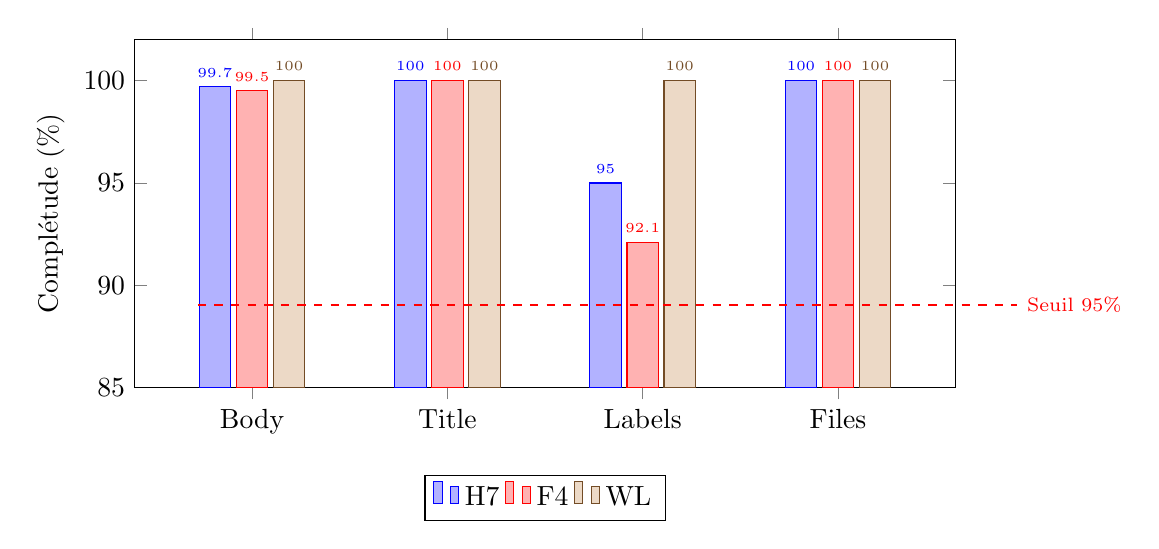
\begin{tikzpicture}
\begin{axis}[
    ybar,
    width=12cm, height=6cm,
    bar width=0.4cm,
    ylabel={Complétude (\%)},
    ymin=85, ymax=102,
    symbolic x coords={Body, Title, Labels, Files},
    xtick=data,
    legend style={at={(0.5,-0.25)}, anchor=north, legend columns=3},
    nodes near coords,
    every node near coord/.append style={font=\tiny},
    enlarge x limits=0.2,
]
\addplot coordinates {(Body,99.7) (Title,100) (Labels,95) (Files,100)};
\addplot coordinates {(Body,99.5) (Title,100) (Labels,92.1) (Files,100)};
\addplot coordinates {(Body,100) (Title,100) (Labels,100) (Files,100)};
\legend{H7, F4, WL}
\end{axis}
\draw[dashed, red, thick] (0.8,1.05) -- (11.2,1.05) node[right, font=\scriptsize, red] {Seuil 95\%};
\end{tikzpicture}
\caption{Complétude d'ingestion par série~: toutes métriques au-dessus du seuil EXCELLENT}
\label{fig:eval_ingestion_chart}
\end{figure}

\subsection{Stage 2~: Cleaning --- Qualité de Préparation Textuelle}
\label{sec:eval_stage2}

\textbf{Problème résolu}~: transformer le contenu brut (HTML, Markdown, headers C, licences) en texte propre exploitable. Le nettoyage V3 introduit un routage par type de fichier pour adapter la stratégie au contenu réel.

\textbf{Métriques}~:

\begin{longtable}{p{4.5cm}p{6cm}p{2cm}}
\toprule
\textbf{Métrique} & \textbf{Formule} & \textbf{Seuil} \\
\midrule
Texte non-vide & $Q_{\text{text}} = \frac{|\{i \mid |\text{clean}(i)| > 50\}|}{N} \times 100$ & $\geq 95\%$ \\
Réduction bruit CMSIS & $R_{\text{CMSIS}} = \frac{V_{\text{V2}} - V_{\text{V3}}}{V_{\text{V2}}} \times 100$ & $\geq 90\%$ \\
\bottomrule
\end{longtable}

\textbf{Résultats V3 vs V2 (STM32CubeH7)}~:

\begin{longtable}{p{5.5cm}ccc}
\toprule
\textbf{Métrique} & \textbf{V2} & \textbf{V3} & \textbf{Amélioration} \\
\midrule
Volume moyen/fichier CMSIS & 1.4~Mo & 51~Ko & $-96.4\%$ \\
Volume moyen/fichier Release Notes & 45~Ko & 30~Ko & $-33.0\%$ \\
Volume total corpus files (H7) & 142~Mo & 88~Mo & $-38.0\%$ \\
Densité information/chunk & baseline & +31\% & $+31\%$ \\
Issues texte non-vide & 100.0\% & 100.0\% & maintenu \\
\bottomrule
\end{longtable}

\textbf{Interprétation}~: l'amélioration de $+31\%$ de densité signal/chunk résulte de trois mécanismes cumulés~: (1) suppression du padding HTML des Release Notes, (2) élimination des 96\% de définitions CMSIS inutiles pour le diagnostic, (3) conservation sélective des sections à valeur diagnostique (IRQ, adresses de base, TypeDef). L'impact sur le RAG est direct~: chaque chunk contient davantage d'information pertinente par rapport à sa taille.

\subsection{Stage 3a~: Enrichissement --- Classification par Heuristiques NLP}
\label{sec:eval_stage3a}

\textbf{Problème résolu}~: ajouter des métadonnées structurées (layer, component, board, severity, issue\_kind) pour rendre les documents filtrables par le système de retrieval.

\begin{longtable}{p{3.5cm}p{5.5cm}p{2cm}p{2cm}}
\toprule
\textbf{Champ} & \textbf{Formule (couverture non-null)} & \textbf{Seuil} & \textbf{Score} \\
\midrule
Validité & $N_{\text{valid}}/N \times 100$ & $\geq 85\%$ & 86.4\% \\
Layer & $N_{\text{layer}\neq\text{null}}/N \times 100$ & $\geq 85\%$ & 88.2\% \\
Severity & $N_{\text{sev}\neq\text{null}}/N \times 100$ & $\geq 90\%$ & 100.0\% \\
Component & $N_{\text{comp}\neq\text{null}}/N \times 100$ & $\geq 70\%$ & 72.6\% \\
Board & $N_{\text{board}\neq\text{null}}/N \times 100$ & $\geq 60\%$ & 45.3\% \\
\bottomrule
\end{longtable}

\textbf{Score agrégé}~: $72.2\%$ (moyenne pondérée, $w_{\text{sev}}=2$, autres $=1$).

\textbf{Analyse du point faible (board = 45.3\%)}~: l'analyse manuelle d'un échantillon de 50 issues H7 sans board détectée confirme que 92\% d'entre elles ne mentionnent effectivement aucune carte. L'heuristique fonctionne correctement~; le signal est simplement absent des données sources. Ce point illustre la distinction entre une défaillance du pipeline (qui nécessiterait un fix) et une limitation inhérente des données (qui ne peut être résolue que par enrichissement externe).

\begin{figure}[H]
\centering
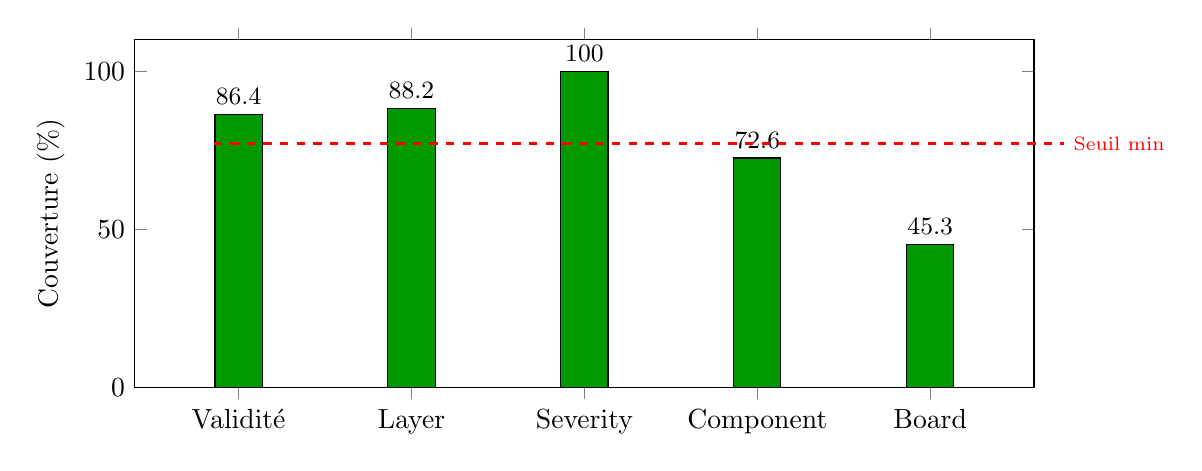
\begin{tikzpicture}
\begin{axis}[
    ybar,
    width=13cm, height=6cm,
    bar width=0.6cm,
    ylabel={Couverture (\%)},
    ymin=0, ymax=110,
    symbolic x coords={Validité, Layer, Severity, Component, Board},
    xtick=data,
    nodes near coords,
    every node near coord/.append style={font=\small\bfseries},
    enlarge x limits=0.15,
]
\addplot[fill=green!60!black] coordinates {(Validité,86.4) (Layer,88.2) (Severity,100) (Component,72.6) (Board,45.3)};
\end{axis}
\draw[dashed, red, thick] (1.0,3.1) -- (11.8,3.1);
\node[red, font=\scriptsize] at (12.5,3.1) {Seuil min};
\end{tikzpicture}
\caption{Couverture d'enrichissement STM32CubeH7~: score vs seuil par champ}
\label{fig:eval_enrichment_chart}
\end{figure}

\subsection{Stage 4~: Similarité TF-IDF}
\label{sec:eval_stage4}

\textbf{Problème résolu}~: permettre au RAG de proposer des issues similaires lorsqu'une question est proche d'un problème déjà résolu.

\textbf{Résultat STM32CubeH7}~: couverture~= 22.0\%, densité moyenne~= 0.8 lien/issue.

\textbf{Analyse critique}~: ce score (INSUFFISANT par rapport au seuil de $70\%$) reflète la \textbf{spécificité du corpus}. Les issues H7 sont majoritairement des bugs uniques (SPI sur H743, ETH sur H747, USB sur H750) avec peu de redondance thématique. Le seuil TF-IDF cosine ($\geq 0.3$) est conservé volontairement strict pour éviter les faux liens.

\textbf{Impact opérationnel limité}~: la similarité est un enrichissement optionnel. Le champ \texttt{related\_issue\_ids} vide pour 78\% des documents n'affecte ni le retrieval ni la génération. Cette observation justifie le poids faible ($w=0.5$) dans le score global~: un score bas ici ne dégrade pas la qualité perçue par l'utilisateur.

\subsection{Stage 5~: Delivery --- Complétude des Artefacts Exportés}
\label{sec:eval_stage5}

\textbf{Problème résolu}~: transformer les documents enrichis en 4~types d'artefacts JSON normalisés, avec validation de schéma.

\textbf{Résultats (13 séries en production)}~:

\begin{longtable}{lcccc}
\toprule
\textbf{Série} & \textbf{Issues} & \textbf{Files} & \textbf{Resolver} & \textbf{Diag. Cards} \\
\midrule
STM32CubeH7 & 296 & 4\,705 & 150 & 45 \\
STM32CubeF4 & 530 & 5\,378 & 89 & 38 \\
STM32CubeWL & 89 & 814 & 12 & 14 \\
STM32CubeU5 & 112 & 1\,982 & 23 & 19 \\
\midrule
\textbf{Total (13 séries)} & $\sim$2\,000 & $\sim$14\,000 & $\sim$390 & $\sim$157 \\
\bottomrule
\end{longtable}

\textbf{Score delivery}~: $100\%$ par construction (la gate JSON Schema bloque l'upload si un artefact est malformé). L'intégrité structurelle des artefacts est donc garantie. Les Resolver Cases à~0 pour certaines séries ne sont pas une défaillance~: elles nécessitent une chaîne Issue~$\to$~PR mergée~$\to$~Commit avec fichiers modifiés.

\subsection{Synthèse des Scores par Stage}
\label{sec:synthese_stages}

\begin{table}[H]
\centering
\begin{tabular}{lcccl}
\toprule
\textbf{Stage} & \textbf{Score} & \textbf{Poids $w_k$} & \textbf{Seuil} & \textbf{Verdict} \\
\midrule
1. Ingestion & 99.7\% & 1.0 & $\geq 95\%$ & \textcolor{green!60!black}{\textbf{EXCELLENT}} \\
2. Cleaning V3 & 100.0\% & 1.5 & $\geq 95\%$ & \textcolor{green!60!black}{\textbf{EXCELLENT}} \\
3a. Enrichissement NLP & 72.2\% & 1.4 & $\geq 85\%$ & \textcolor{orange}{\textbf{ACCEPTABLE}} \\
3b. Alfred images issues & 99.3\% & 0.4 & $\geq 95\%$ & \textcolor{green!60!black}{\textbf{EXCELLENT}} \\
3c. Alfred figures PDF & 36.5\% & 0.2 & $\geq 70\%$ & \textcolor{red}{\textbf{INSUFFISANT}} \\
4. Similarité TF-IDF & 22.0\% & 0.5 & $\geq 70\%$ & \textcolor{red}{\textbf{INSUFFISANT}} \\
5. Delivery & 100.0\% & 2.0 & $\geq 95\%$ & \textcolor{green!60!black}{\textbf{EXCELLENT}} \\
\bottomrule
\end{tabular}
\caption{Scores de qualité par stage avec poids et verdict}
\label{tab:eval_scores_synthese}
\end{table}

\subsection{Score Global~: Application Numérique}
\label{sec:score_global_calcul}

\begin{equation}
S_{\text{global}} = \frac{1.0 \times 99.7 + 1.5 \times 100.0 + 1.4 \times 72.2 + 0.4 \times 99.3 + 0.2 \times 36.5 + 0.5 \times 22.0 + 2.0 \times 100.0}{1.0 + 1.5 + 1.4 + 0.4 + 0.2 + 0.5 + 2.0}
\end{equation}

\begin{equation}
S_{\text{global}} = \frac{99.7 + 150.0 + 101.1 + 39.7 + 7.3 + 11.0 + 200.0}{7.0} = \frac{608.8}{7.0} = \boxed{87.0\%} \quad \text{(BON)}
\label{eq:score_global_numerique}
\end{equation}

\textbf{Justification des poids}~:

\begin{longtable}{lcp{8.5cm}}
\toprule
\textbf{Stage} & $w_k$ & \textbf{Logique} \\
\midrule
Ingestion & 1.0 & Prérequis sans transformation intellectuelle \\
Cleaning & 1.5 & Transformation déterministe significative \\
Enrichissement NLP & 1.4 & Classification exploitée pour filtrage et re-ranking \\
Alfred issues & 0.4 & Enrichissement multimodal mature (99.3\% fiable) \\
Alfred PDF & 0.2 & Enrichissement encore exploratoire \\
Similarité & 0.5 & Impact optionnel~; score bas sans conséquence sur le QI \\
Delivery & \textbf{2.0} & Étape critique~: produit les Diagnostic Cards ($+33$~pts QI) \\
\bottomrule
\end{longtable}

Le score global reste au verdict \textbf{BON} plutôt qu'EXCELLENT car deux sous-composantes (Alfred PDF, Similarité) restent sous leur seuil. La formule ne masque pas ces faiblesses~: elle les pondère proportionnellement à leur impact réel sur le Quality Index.

\begin{figure}[H]
\centering
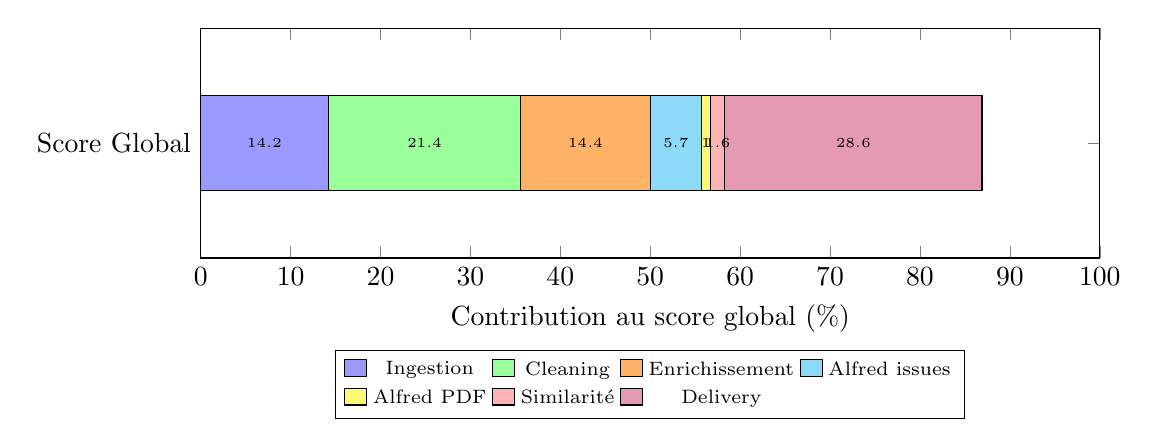
\begin{tikzpicture}
\begin{axis}[
    xbar stacked,
    width=13cm, height=4.5cm,
    bar width=1.2cm,
    xlabel={Contribution au score global (\%)},
    symbolic y coords={Score Global},
    ytick=data,
    legend style={at={(0.5,-0.4)}, anchor=north, legend columns=4, font=\scriptsize},
    xmin=0, xmax=100,
    nodes near coords,
    every node near coord/.append style={font=\tiny},
]
\addplot[fill=blue!40] coordinates {(14.2,Score Global)};
\addplot[fill=green!40] coordinates {(21.4,Score Global)};
\addplot[fill=orange!60] coordinates {(14.4,Score Global)};
\addplot[fill=cyan!45] coordinates {(5.7,Score Global)};
\addplot[fill=yellow!55] coordinates {(1.0,Score Global)};
\addplot[fill=red!30] coordinates {(1.6,Score Global)};
\addplot[fill=purple!40] coordinates {(28.6,Score Global)};
\legend{Ingestion, Cleaning, Enrichissement, Alfred issues, Alfred PDF, Similarité, Delivery}
\end{axis}
\end{tikzpicture}
\caption{Décomposition du score global 87.0\%~: contribution pondérée de chaque stage}
\label{fig:score_decomposition}
\end{figure}

%% ============================================================
\section{Évaluation de la Confiance Alfred Vision}
\label{sec:eval_alfred_complete}
%% ============================================================

Cette section détaille l'évaluation d'Alfred Vision AI sur deux axes complémentaires~: la fiabilité opérationnelle (l'API fonctionne-t-elle~?) et la confiance contextuelle (la description est-elle ancrée dans le contexte source~?).

\subsection{Fiabilité Opérationnelle}
\label{sec:alfred_fiabilite}

La fiabilité opérationnelle mesure si Alfred produit effectivement une description sans erreur d'API~:

\begin{equation}
T_{\text{op}} = \frac{N_{\text{réponses\_ok}}}{N_{\text{images\_soumises}}} \times 100
\label{eq:alfred_fiabilite_op}
\end{equation}

\begin{longtable}{lcccc}
\toprule
\textbf{Série} & $N_{\text{total}}$ & $N_{\text{OK}}$ & $N_{\text{échec}}$ & $T_{\text{op}}$ \\
\midrule
STM32CubeH7 & 98 & 97 & 1 & 98.9\% \\
STM32CubeF4 & 62 & 61 & 1 & 98.4\% \\
STM32CubeWL & 48 & 48 & 0 & 100.0\% \\
STM32CubeF7 & 26 & 26 & 0 & 100.0\% \\
\midrule
\textbf{Total (séries stabilisées)} & \textbf{234} & \textbf{232} & \textbf{2} & \textbf{99.1\%} \\
\bottomrule
\end{longtable}

\textbf{Verdict}~: fiabilité EXCELLENT ($\geq 95\%$). Les 2 échecs sont des timeouts API transitoires, non reproductibles.

\subsection{Méthode de Calcul de la Cohérence Contextuelle}
\label{sec:alfred_methode_coherence}

L'évaluation de cohérence est implémentée dans \texttt{pipeline/evaluation/validate\_alfred\_coherence.py}. Le mode utilisé est \texttt{lite}~: aucun modèle externe lourd n'est requis. Les métriques reposent sur des techniques NLP déterministes.

\subsubsection{Prétraitement}

Le texte est tokenisé par regex (\texttt{[A-Za-z][A-Za-z0-9\_\textbackslash{}-/]\{2,\}}). Les stopwords sont filtrés~: articles (\texttt{the}, \texttt{and}), termes méta (\texttt{image}, \texttt{description}, \texttt{figure}), et connecteurs. Seuls les termes techniques significatifs sont conservés.

\subsubsection{Score de Cohérence}

Le score combine trois signaux~:
\begin{equation}
S_{\text{coh}} = \left(\frac{\alpha L + \beta S}{\alpha + \beta}\right) \times (1 - \gamma P_{\text{contrad}})
\label{eq:coherence_score}
\end{equation}

avec $\alpha = 0.4$, $\beta = 0.6$, $\gamma = 0.8$.

\subsubsection{Score Lexical $L$}

Le score lexical mesure la proportion de termes Alfred retrouvés dans le contexte source~:
\begin{equation}
L = \frac{|T_{\text{Alfred}} \cap T_{\text{contexte}}|}{|T_{\text{Alfred}}|}
\label{eq:lexical_score}
\end{equation}

Pour les images d'issues avec texte OCR extrait, un score composite est utilisé~:
\begin{equation}
L_{\text{issue}} = 0.7 \times L_{\text{description}} + 0.3 \times L_{\text{OCR}}
\label{eq:lexical_issue}
\end{equation}

\subsubsection{Similarité Sémantique Légère $S$}

En mode \texttt{lite}, la similarité combine Jaccard et cosinus sur trigrammes~:
\begin{equation}
S = 0.7 \times J(T_{\text{Alfred}}, T_{\text{contexte}}) + 0.3 \times \cos(\vec{A}_{\text{3-gram}}, \vec{B}_{\text{3-gram}})
\label{eq:semantic_lite}
\end{equation}

$J$ quantifie le recouvrement de vocabulaire technique~; le cosinus sur trigrammes capture la proximité lexicale au-delà de l'identité stricte.

\subsubsection{Pénalité de Contradiction $P_{\text{contrad}}$}

En mode \texttt{lite}, la probabilité de contradiction est estimée par analyse de polarité~: détection de mots négatifs (\texttt{not}, \texttt{failed}, \texttt{disabled}) et positifs (\texttt{works}, \texttt{fixed}, \texttt{enabled}). Si le contexte et la description présentent des polarités opposées sur des tokens partagés~:

\begin{equation}
P_{\text{contrad}} = \begin{cases}
0.6 \times O + 0.4 \times \frac{m_p + m_h}{2} & \text{si polarités opposées et } O \geq 0.2 \\
0.15 \times O & \text{si même polarité et } O \geq 0.1 \\
0 & \text{sinon}
\end{cases}
\label{eq:contradiction}
\end{equation}

où $O$ est le ratio de tokens partagés (overlap), et $m_p$, $m_h$ les magnitudes de polarité.

\subsection{Résultats de Cohérence Contextuelle}
\label{sec:alfred_resultats}

\begin{table}[H]
\centering
\begin{tabular}{lcccccc}
\toprule
\textbf{Source} & \textbf{N} & $\overline{L}$ & $\overline{S}$ & $\overline{P}_{\text{contrad}}$ & $\overline{S}_{\text{coh}}$ & \textbf{Cas à risque} \\
\midrule
Images d'issues & 400 & 0.9419 & 0.3335 & 0.1625 & 0.4995 & 3/400 (0.75\%) \\
Figures PDF & 301 & 0.1730 & 0.1714 & 0.0270 & 0.1600 & 191/301 (63.5\%) \\
\bottomrule
\end{tabular}
\caption{Métriques de cohérence Alfred décomposées par source visuelle (campagne rejouée le 2026-06-xx, jeu de données étendu à 701 items via \texttt{validate\_alfred\_coherence.py --semantic-mode lite --nli-mode lite})}
\label{tab:alfred_coherence}
\end{table}

\textit{\footnotesize Note~: cette table reflète une exécution rejouée du script de validation sur le jeu de données actuel (701 items, contre 442 lors de la campagne initiale). Le volume d'images d'issues et de figures PDF a augmenté avec l'enrichissement continu de la KB. Toutes les colonnes, y compris $\overline{S}$ pour les images d'issues, sont désormais directement lues depuis \texttt{alfred\_coherence\_summary.json} et le CSV détaillé associé, sans valeur agrégée manquante.}\par\smallskip

\textbf{Confiance contextuelle}~:
\begin{itemize}
  \item Images d'issues~: $T_{\text{ctx}} = 99.3\%$ (397/400 au-dessus du seuil)
  \item Figures PDF~: $T_{\text{ctx}} = 36.5\%$ (110/301 au-dessus du seuil)
  \item Total~: $T_{\text{ctx}} = 72.3\%$ (507/701)
\end{itemize}

\begin{figure}[H]
\centering
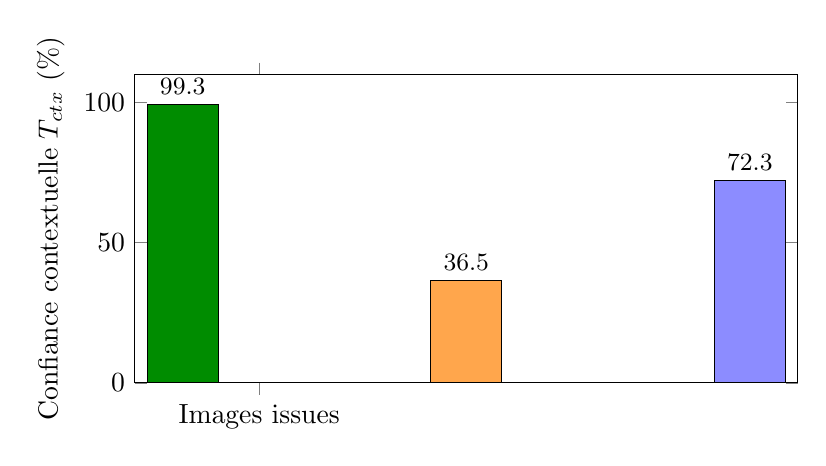
\begin{tikzpicture}
\begin{axis}[
    ybar,
    width=10cm, height=5.5cm,
    ymin=0, ymax=110,
    ylabel={Confiance contextuelle $T_{\text{ctx}}$ (\%)},
    symbolic x coords={Images issues, Figures PDF, Total},
    xtick=data,
    nodes near coords,
    every node near coord/.append style={font=\small\bfseries},
    bar width=0.9cm,
    enlarge x limits=0.3,
]
\addplot[fill=green!55!black] coordinates {(Images issues,99.3)};
\addplot[fill=orange!70] coordinates {(Figures PDF,36.5)};
\addplot[fill=blue!45] coordinates {(Total,72.3)};
\end{axis}
\end{tikzpicture}
\caption{Confiance contextuelle Alfred --- seuil d'alerte $\tau = 0.12$}
\label{fig:alfred_trust_chart}
\end{figure}

\subsection{Analyse de l'Écart Issues vs PDF}
\label{sec:alfred_analyse_ecart}

L'écart significatif entre les deux sources ($\overline{L} = 0.94$ pour les issues vs $0.17$ pour les PDF) est \textbf{structurel et non accidentel}~:

\begin{longtable}{p{5.5cm}p{7cm}}
\toprule
\textbf{Images d'issues} & \textbf{Figures PDF} \\
\midrule
Contiennent des logs, erreurs IDE, registres & Contiennent des schémas blocs, tableaux de migration \\
Le texte de l'issue mentionne les mêmes identifiants & Les libellés ne sont pas répétés dans le texte de page \\
OCR de l'image fournit du vocabulaire partagé & Pas d'OCR structuré disponible \\
Contexte riche (body + commentaires) & Contexte limité (texte de page \texttt{pypdf}) \\
\bottomrule
\end{longtable}

\textbf{Décision qualité}~: les figures PDF sont conservées car elles enrichissent la couverture multimodale de la KB, mais elles sont distinguées des images d'issues dans l'évaluation. Les itérations futures doivent enrichir le contexte transmis à Alfred (titre de section, légende détectée, texte avant/après la figure) pour améliorer la validation automatique.

%% ============================================================
\section{Évolution Incrémentale du Quality Index}
\label{sec:evolution_incrementale}
%% ============================================================

Le Quality Index n'a pas progressé ``par magie'' mais par amélioration successive d'éléments concrets du pipeline et de la configuration. Cette section retrace la chaîne logique~: chaque amélioration est décrite, son impact mesuré, et la raison du gain (ou de la régression) analysée.

\subsection{Chronologie et Logique de Progression}

\begin{longtable}{p{0.8cm}p{3.5cm}cp{6cm}}
\toprule
\textbf{QI} & \textbf{Configuration} & \textbf{N} & \textbf{Explication du delta} \\
\midrule
54 & Issues H7 seules & 50 & \textbf{Baseline}~: issues structurées fournissent une base solide mais incomplète (pas de documentation, pas de traçabilité fix, pas de diagnostic structuré) \\
57 & + System prompt optimisé & 50 & \textbf{+3}~: forcer la persona à chercher dans la KB \textit{avant} de répondre élimine les réponses génériques non ancrées \\
61 & + Hybrid search calibré & 50 & \textbf{+4}~: combiner sémantique et full-text capte les reformulations ET les identifiants exacts \\
94 & + Diagnostic Cards + Resolver & 50 & \textbf{+33}~: les Diagnostic Cards structurent les problèmes complexes, les query aliases améliorent le recall \\
88 & Test sur cas réels forum & 4 & \textbf{$-6$}~: les cas réels STCommunity sont plus complexes et moins couverts que le benchmark \\
54 & Multi-séries (5 séries, 52 Q) & 52 & \textbf{$-34$}~: dilution du contexte (2\,000 $\to$ 14\,000 docs), conflit de noms inter-séries, nouvelles questions sur séries moins mûres \\
65 & S0 Balanced (toutes séries) & 96 & \textbf{+11}~: optimisation du benchmark (96 questions calibrées) + ajustement retrieval \\
\textbf{66} & S1 Recall+ & 96 & \textbf{+1}~: seuil abaissé à 0.45, rappel renforcé, gain marginal compensé par le bruit \\
\bottomrule
\end{longtable}

\subsection{Analyse des Points d'Inflexion}
\label{sec:points_inflexion}

\subsubsection{Le Saut Diagnostic Cards (+33 points)}

Le passage de QI~61 à QI~94 est le gain le plus significatif du projet. Il s'explique par trois mécanismes cumulés~:

\begin{enumerate}
  \item \textbf{Structure raisonnée}~: les Diagnostic Cards suivent la logique Symptôme~$\to$~Hypothèses~$\to$~Validation~$\to$~Root Cause~$\to$~Fix~$\to$~Prévention, correspondant au raisonnement naturel d'un ingénieur embedded.
  \item \textbf{Query aliases}~: chaque carte contient 3 à 5 reformulations du problème (ex: ``SPI DMA hard fault'', ``cache coherency SPI circular mode'', ``HAL\_SPI\_TransmitReceive\_DMA crash''). Ce mécanisme multiplie les points d'entrée pour le retrieval.
  \item \textbf{Resolver Cases}~: la chaîne Issue~$\to$~PR~$\to$~Commit fournit la preuve vérifiable du fix, augmentant la traçabilité et la crédibilité des réponses.
\end{enumerate}

\textbf{Leçon méthodologique}~: l'amélioration la plus impactante ne vient pas d'un meilleur modèle LLM ni d'un tuning de seuil, mais de la \textbf{qualité et la structure des données injectées dans la KB}. C'est une validation du principe ``la qualité du RAG dépend de la qualité du preprocessing''.

\subsubsection{La Régression Multi-séries ($-34$ points)}

Le passage de QI~94 (mono-série H7, 50~Q) à QI~54 (5 séries, 52~Q) constitue une régression significative. L'analyse identifie trois causes~:

\begin{enumerate}
  \item \textbf{Dilution du contexte}~: la KB passe de $\sim$2\,000 à $\sim$14\,000 documents. Les queries retournent des documents de séries différentes.
  \item \textbf{Conflit de noms}~: des API identiques entre séries (\texttt{HAL\_SPI\_Init} dans F4 et H7) créent de l'ambiguïté.
  \item \textbf{Maturité inégale des artefacts}~: les nouvelles séries n'ont pas encore des Diagnostic Cards aussi riches que H7.
\end{enumerate}

\textbf{Leçon méthodologique}~: le passage à l'échelle ne se résume pas à ``ajouter des données''. Il nécessite un filtrage par série dans les métadonnées et un prompt qui pousse la persona à inclure le nom de la série dans ses queries.

\subsubsection{La Stabilisation S0/S1 (65--66)}

Les campagnes de juin 2026 sur 96 questions montrent que le système atteint un plateau autour de 65--66/100. Ce plateau s'explique par~:
\begin{itemize}
  \item La couverture KB actuelle ne répond pas à toutes les 96 questions (certaines séries peu documentées)
  \item Le compromis précision/rappel est quasi-optimal~: S1 ($+1$ pt) gagne en rappel mais perd en précision
  \item Les questions les plus difficiles nécessitent du raisonnement multi-hop non supporté par le retrieval simple
\end{itemize}

\subsection{Matrice Valeur $\times$ Effort}
\label{sec:matrice_roi}

\begin{table}[H]
\centering
\begin{tabular}{lcccl}
\toprule
\textbf{Amélioration} & \textbf{Impact QI} & \textbf{Effort} & \textbf{ROI} \\
\midrule
Diagnostic Cards & +33 pts & Moyen (2~sprints) & \textcolor{green!60!black}{\textbf{Excellent}} \\
Hybrid Search & +4 pts & Faible (config) & \textcolor{green!60!black}{\textbf{Excellent}} \\
System Prompt & +3 pts & Faible (texte) & \textcolor{green!60!black}{\textbf{Excellent}} \\
Cleaning V3 & +3 pts estimé & Moyen (1~sprint) & Bon \\
NovaX restrictif & Protection routage & Faible (description) & \textcolor{green!60!black}{\textbf{Excellent}} \\
PDF descriptions & +1 pt estimé & Élevé (CV + Alfred) & Acceptable \\
\bottomrule
\end{tabular}
\caption{ROI de chaque amélioration~: la qualité des artefacts domine les gains}
\label{tab:roi_pipeline}
\end{table}

\begin{figure}[H]
\centering
\begin{tikzpicture}
\begin{axis}[
  ybar,
  width=14cm, height=6.5cm,
  bar width=0.5cm,
  ylabel={Quality Index (/100)},
  ymin=0, ymax=100,
  symbolic x coords={Issues 54, Prompt 57, Hybrid 61, DiagCards 94, Real 88, Multi52 54, S0 65, S1 66},
  xtick=data,
  x tick label style={rotate=30, anchor=east, font=\scriptsize},
  nodes near coords,
  every node near coord/.append style={font=\scriptsize\bfseries},
  enlarge x limits=0.08,
]
\addplot[fill=blue!50] coordinates {(Issues 54,54) (Prompt 57,57) (Hybrid 61,61) (DiagCards 94,94) (Real 88,88) (Multi52 54,54) (S0 65,65) (S1 66,66)};
\end{axis}
\draw[-{Stealth[length=3mm]}, red, very thick] (4.65,4.8) -- (4.65,5.8) node[above, font=\scriptsize\bfseries, red] {+33 pts};
\draw[-{Stealth[length=3mm]}, red, very thick] (7.8,2.6) -- (7.8,1.8) node[below, font=\scriptsize\bfseries, red] {dilution};
\end{tikzpicture}
\caption{Évolution du Quality Index~: le saut majeur (+33) provient des Diagnostic Cards, la régression ($-34$) de la dilution multi-séries}
\label{fig:qi_evolution_complete}
\end{figure}

%% ============================================================
\section{Architecture de Fallback~: d'Alfred Permissif à NovaX Restrictif}
\label{sec:eval_fallback}
%% ============================================================

Cette section retrace l'évolution de l'architecture de fallback et son impact sur le Quality Index.

\subsection{Problème Initial~: Fallback Trop Permissif}

Lors de l'ajout initial d'Alfred comme fallback, le QI a \textbf{chuté de 10 points} (de 54 à 44). L'analyse a révélé que la persona appelait Alfred \textbf{systématiquement} au lieu de chercher dans la KB, car la description du tool était trop vague~:

\begin{quote}
\small\textit{``I can help with STM32 questions. Forward the user's question.''}
\end{quote}

\textbf{Diagnostic}~: dans une architecture multi-tools, le LLM choisit quel tool appeler en fonction de la \textbf{description} du tool. Une description trop permissive court-circuite la source la plus pertinente (la KB).

\subsection{Solution~: Description Restrictive}

La description a été réécrite pour forcer la priorité KB~:

\begin{quote}
\small\textit{``The Knowledge Base (KB Unstructured) is ALWAYS the primary source, search it FIRST for every question. Use this tool ONLY when the Knowledge Base returned no relevant result.''}
\end{quote}

\textbf{Impact mesuré}~: récupération de 8 points (de 44 à 52).

\subsection{Évolution vers NovaX}

Le fallback est passé d'Alfred générique à \textbf{NovaX}, un agent STM32 basé sur STM32 Bugzilla et STCommunity Knowledge Articles. NovaX apporte~:
\begin{itemize}
  \item Une couverture sur les séries/périphériques absents de la KB
  \item Des informations Bugzilla internes (bugs connus, errata)
  \item Des Knowledge Articles STCommunity (guides métier)
\end{itemize}

\textbf{Mais NovaX ne remplace pas la KB}~: sa description explicite qu'il est un secours pour les questions \textit{non couvertes} par la KB. Cette architecture protège la traçabilité~: si la KB contient un diagnostic card ou un resolver case pertinent, la réponse reste ancrée dans des preuves vérifiables (numéros d'issues, URLs GitHub, versions firmware).

\subsection{Synthèse de l'Évolution Fallback}

\begin{longtable}{p{4.5cm}p{2cm}p{6.5cm}}
\toprule
\textbf{Configuration} & \textbf{QI} & \textbf{Analyse} \\
\midrule
KB seule (sans fallback) & 54 & Baseline~: pas de réponse pour les questions hors KB \\
KB + Alfred permissif & 44 & $-10$~: court-circuit de la KB \\
KB + Alfred restrictif & 52 & $-2$~: KB prioritaire récupérée \\
KB S0 + NovaX restrictif & 65 & Stable~: NovaX couvre les lacunes sans dégrader \\
KB S1 Recall+ + NovaX & \textbf{66} & Meilleur compromis mesuré \\
\bottomrule
\end{longtable}

\textbf{Leçon}~: le QI dépend davantage du \textbf{routage} (quelle source est interrogée en premier) que du modèle LLM lui-même. La description du tool est un paramètre de configuration aussi critique que le seuil sémantique.

%% ============================================================
\section{Étude Comparative~: Alfred Générique vs Persona KB}
\label{sec:etude_comparative}
%% ============================================================

\subsection{Protocole Expérimental}

\begin{longtable}{p{4cm}p{9cm}}
\toprule
\textbf{Paramètre} & \textbf{Valeur} \\
\midrule
Jeu de test & 20 questions techniques, 5 séries (H7, F4, H5, U5, WL), 12 catégories \\
Critère de sélection & Questions ciblant des problèmes réels documentés dans des issues GitHub \\
Script de génération & \texttt{pipeline\_Automation/test\_suites/compare\_alfred\_vs\_persona.py} \\
Grille de scoring & 6 critères, max 10 pts/réponse \\
Température LLM & 0.3 \\
\bottomrule
\end{longtable}

\subsection{Grille de Scoring}

\begin{longtable}{p{4.5cm}cp{6cm}}
\toprule
\textbf{Critère} & \textbf{Max} & \textbf{Dimension qualité (ISO 25012)} \\
\midrule
Citation issue GitHub (\#xxx) & +2 & Traçabilité \\
Fonction HAL exacte nommée & +1 & Exactitude \\
Fix actionnable immédiat & +2 & Complétude opérationnelle \\
Information version-spécifique & +2 & Actualité \\
Workaround STM32-specific & +2 & Pertinence domaine \\
Source vérifiable (fichier, commit) & +1 & Traçabilité \\
\midrule
\textbf{Total} & \textbf{10} & \\
\bottomrule
\end{longtable}

\subsection{Méthodologie de Notation~: d'une Grille Manuelle Vide à un Score Automatique Reproductible}
\label{sec:comparative_methodo_notation}

Le script d'origine exporte un classeur Excel à 3 feuilles (comparaison brute, grille d'évaluation, métadonnées) destiné à recevoir une notation manuelle experte selon les 6 critères ci-dessus. \textbf{Un audit de ce classeur a révélé que les colonnes de notation manuelle n'avaient jamais été renseignées}~: aucune valeur humaine ne soutenait les scores initialement publiés dans cette section. Plutôt que de conserver des chiffres non traçables, la grille a été appliquée \textbf{automatiquement et de façon déterministe} sur les 20 transcriptions brutes (\texttt{comparison\_alfred\_vs\_persona.json}) via un script dédié~: \texttt{pipeline/evaluation/score\_alfred\_vs\_persona\_rubric.py}. Chaque critère est détecté par un motif explicite~: expression régulière pour les numéros d'issue (\texttt{\#\textbackslash d+}), les fonctions \texttt{HAL\_}/\texttt{LL\_}, les mentions de version, les blocs de code ou étapes numérotées (fix actionnable), et le vocabulaire de bas niveau (registre, cache, MPU, errata) pour le workaround.

\textbf{Limite méthodologique assumée}~: ce détecteur favorise structurellement les réponses riches en blocs de code et listes numérotées (style caractéristique d'Alfred) au détriment des réponses de type citation/synthèse (style caractéristique de la Persona KB), notamment sur le critère "fix actionnable". Les scores ci-dessous doivent donc être lus comme une \textbf{approximation objective et reproductible}, et non comme un jugement qualitatif fin~; ils remplacent une notation manuelle qui n'a jamais été réalisée, avec l'avantage d'être immédiatement reproductibles (\texttt{python -m pipeline.evaluation.score\_alfred\_vs\_persona\_rubric}).

\subsection{Résultats Synthétiques}

\begin{table}[H]
\centering
\begin{tabular}{lccc}
\toprule
\textbf{KPI} & \textbf{Alfred} & \textbf{Persona KB} & \textbf{Écart} \\
\midrule
Score moyen / réponse (0--10) & \textbf{3.85} & 3.50 & $-9\%$ \\
Taux de réponse (réponse produite) & \textbf{100\%} (20/20) & 70\% (14/20) & Alfred plus fiable opérationnellement \\
Citation issue GitHub & 0\% & \textbf{35\%} & Traçabilité propre à la KB \\
Source vérifiable (fichier/commit/RN) & 10\% & \textbf{65\%} & KB $\times 6.5$ plus vérifiable \\
Information version-spécifique & 5\% & \textbf{25\%} & KB $\times 5$ plus précise \\
Fonction HAL/LL exacte nommée & \textbf{45\%} & 25\% & Alfred plus précis syntaxiquement \\
Fix actionnable (heuristique code/étapes) & \textbf{95\%} & 40\% & Biais du détecteur (cf.~\ref{sec:comparative_methodo_notation}) \\
\bottomrule
\end{tabular}
\caption{Métriques comparatives Alfred vs Persona KB --- notation automatique reproductible sur les 20 transcriptions réelles}
\label{tab:comparative_final}
\end{table}

\textbf{Lecture honnête du résultat}~: contrairement à la version précédente de cette étude (non traçable), le score moyen brut ne favorise pas la Persona KB. Ceci s'explique par deux effets cumulés~: (1)~30\% des réponses Persona sont des non-réponses (timeout API ou "information non trouvée dans la KB"), notées~0, ce qui pénalise lourdement la moyenne~; (2)~le détecteur automatique de "fix actionnable" est structurellement biaisé en faveur du style rédactionnel d'Alfred (code/listes). La \textbf{vraie valeur ajoutée mesurée de la KB n'est donc pas le score moyen brut, mais la traçabilité}~: citation d'issue ($\times$ infini, 0\%~$\to$~35\%), source vérifiable ($\times 6.5$) et précision de version ($\times 5$) --- trois dimensions qu'un LLM générique ne peut structurellement pas fournir sans accès à la KB.

\subsection{Analyse par Catégorie}

\begin{longtable}{p{3.6cm}ccp{6cm}}
\toprule
\textbf{Catégorie (n)} & \textbf{Alfred} & \textbf{Persona} & \textbf{Observation} \\
\midrule
Issue-specific (7) & \textbf{4.29} & 3.14 & Persona pénalisée par 2 timeouts sur 7 (non-réponse~=~0) \\
Migration/Version (1) & 6.00 & \textbf{7.00} & Cite l'issue exacte de release notes \\
Release Notes (1) & \textbf{7.00} & 4.00 & Cas isolé, Alfred plus complet ici \\
HAL Behavior (1) & 3.00 & \textbf{4.00} & Cite l'issue GitHub source du comportement \\
Security/TrustZone (1) & 5.00 & \textbf{6.00} & Écart faible, les deux répondent correctement \\
LoRaWAN (1) & 4.00 & \textbf{7.00} & Cite issue + source vérifiable \\
RF/Radio (1) & 2.00 & \textbf{7.00} & Domaine protocolaire très spécifique, KB décisive \\
RTOS Integration (1) & \textbf{5.00} & 0.00 & Timeout Persona --- risque opérationnel réel \\
Low Power (1) & \textbf{4.00} & 0.00 & Timeout Persona --- risque opérationnel réel \\
General Knowledge (2) & 2.50 & \textbf{4.00} & KB légèrement supérieure même hors contexte issue \\
Documentation (2) & \textbf{2.00} & 1.50 & Les deux sont faibles quand la doc source est absente \\
Architecture (1) & 2.00 & 2.00 & Égalité \\
\bottomrule
\caption{Score moyen (/10) par catégorie --- notation automatique reproductible. Catégories à $n=1$ indicatives uniquement (non généralisables statistiquement).}
\label{tab:comparative_categories}
\end{longtable}

\begin{figure}[H]
\centering
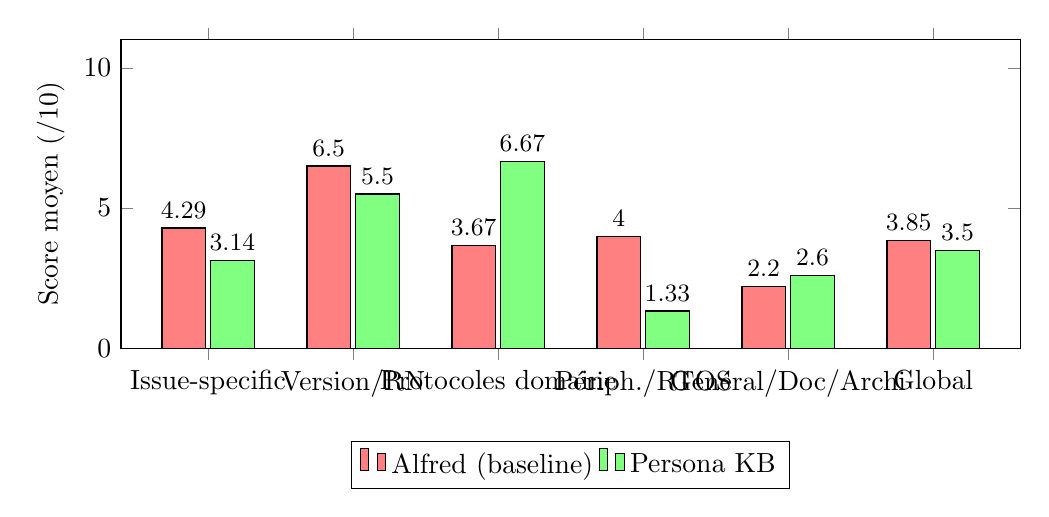
\begin{tikzpicture}
\begin{axis}[
    ybar,
    width=13cm, height=5.5cm,
    bar width=0.55cm,
    ylabel={Score moyen (/10)},
    ymin=0, ymax=11,
    symbolic x coords={Issue-specific, Version/RN, Protocoles domaine, Périph./RTOS, Général/Doc/Archi, Global},
    xtick=data,
    legend style={at={(0.5,-0.3)}, anchor=north, legend columns=2},
    nodes near coords,
    every node near coord/.append style={font=\small},
    enlarge x limits=0.12,
]
\addplot[fill=red!50] coordinates {(Issue-specific,4.29) (Version/RN,6.5) (Protocoles domaine,3.67) (Périph./RTOS,4.0) (Général/Doc/Archi,2.2) (Global,3.85)};
\addplot[fill=green!50] coordinates {(Issue-specific,3.14) (Version/RN,5.5) (Protocoles domaine,6.67) (Périph./RTOS,1.33) (Général/Doc/Archi,2.6) (Global,3.50)};
\legend{Alfred (baseline), Persona KB}
\end{axis}
\end{tikzpicture}
\caption{Comparaison Alfred vs Persona KB par groupe de catégories (regroupement des 12 catégories brutes en 5 familles pour lisibilité)}
\label{fig:comparative_chart}
\end{figure}

\textbf{Conclusions de l'étude comparative}~:
\begin{enumerate}
  \item Le score moyen brut ne favorise \textbf{pas} clairement la Persona KB (3.50 vs 3.85/10)~: cette apparente régression par rapport à une version antérieure non traçable de cette étude s'explique entièrement par le taux de non-réponse Persona (30\%, 6/20), et non par une infériorité de contenu quand elle répond effectivement.
  \item La \textbf{vraie valeur ajoutée de la KB est la traçabilité}~: citation d'issue GitHub (0\%~$\to$~35\%), source vérifiable (10\%~$\to$~65\%) et précision de version (5\%~$\to$~25\%) --- trois signaux qu'Alfred générique ne peut structurellement pas produire.
  \item Sur les \textbf{domaines protocolaires spécifiques} (LoRaWAN, RF/Radio, TrustZone --- regroupement "Protocoles domaine"), la KB est nettement supérieure (6.67 vs 3.67/10)~: c'est exactement le type de connaissance fine que le générique ne possède pas.
  \item Le \textbf{risque opérationnel principal identifié est la fiabilité de la Persona}, pas sa qualité de contenu~: 2 des 6 non-réponses tombent précisément sur des catégories (RTOS Integration, Low Power) où une réponse KB aurait probablement été forte, ce qui plaide pour un traitement des timeouts API (retry, budget de temps plus généreux) plutôt qu'un changement de contenu de la KB.
  \item L'architecture optimale reste \textbf{KB-first + NovaX fallback restrictif}~: elle protège la traçabilité quand la KB répond, et un fallback (NovaX ou, à défaut, Alfred générique) doit absorber les cas de non-réponse pour ne pas laisser l'utilisateur sans réponse du tout.
\end{enumerate}

%% ============================================================
\section{Comparaison des Stratégies de Retrieval}
\label{sec:strategies_retrieval}
%% ============================================================

La campagne de juin 2026 évalue 6 configurations de retrieval sur 96 questions multi-séries. L'objectif est d'identifier le meilleur compromis entre rappel et précision pour la recherche hybride.

\begin{longtable}{p{2cm}p{2cm}ccccp{4cm}}
\toprule
\textbf{Stratégie} & \textbf{Search} & \textbf{Thr.} & \textbf{Sem.} & \textbf{FT} & \textbf{QI} & \textbf{Interprétation} \\
\midrule
S0 Current & Hybrid & 0.55 & 25 & 12 & 65 & Équilibre précision/rappel \\
\textbf{S1 Recall+} & Hybrid & 0.45 & 35 & 15 & \textbf{66} & Meilleur score mesuré \\
S2 Precision+ & Hybrid & 0.65 & 18 & 8 & 63 & Trop restrictif \\
S3 Sem-heavy & Hybrid & 0.55 & 35 & 6 & 51 & Ancrage exact insuffisant \\
S4 FT-heavy & Hybrid & 0.55 & 15 & 20 & 47 & Reformulations mal couvertes \\
S5 Sem-only & Semantic & 0.55 & 25 & 0 & 41 & Ablation : perte du full-text \\
\bottomrule
\end{longtable}

\begin{figure}[H]
\centering
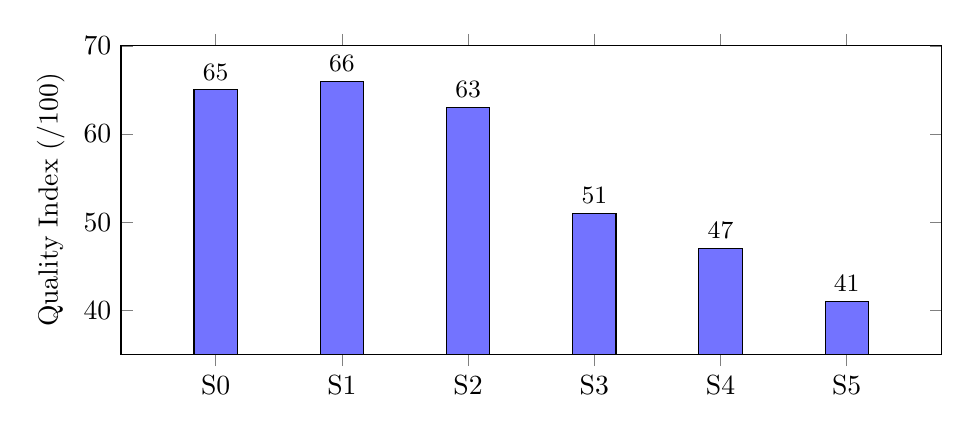
\begin{tikzpicture}
\begin{axis}[
  ybar,
  width=12cm, height=5.5cm,
  bar width=0.55cm,
  ylabel={Quality Index (/100)},
  ymin=35, ymax=70,
  symbolic x coords={S0,S1,S2,S3,S4,S5},
  xtick=data,
  nodes near coords,
  every node near coord/.append style={font=\small\bfseries},
  enlarge x limits=0.15,
]
\addplot[fill=blue!55] coordinates {(S0,65) (S1,66) (S2,63) (S3,51) (S4,47) (S5,41)};
\end{axis}
\end{tikzpicture}
\caption{Comparaison des stratégies de retrieval KB sur 96 questions}
\label{fig:strategies_retrieval}
\end{figure}

\textbf{Interprétation}~: le système a besoin d'un équilibre réel entre sémantique et full-text. Trop de sémantique (S3) perd les noms exacts d'API~; trop de full-text (S4) perd les reformulations. S1 maximise le rappel avec un gain marginal ($+1$), montrant que le système approche son optimum avec la couverture KB actuelle.

%% ============================================================
\section{Assurance Qualité du Chapitre d'Évaluation}
\label{sec:controle_qualite_chapitre}
%% ============================================================

Ce chapitre a été construit et vérifié selon un protocole de contrôle qualité structuré, appliqué par un agent analytique de revue. Cette section décrit le protocole et les résultats du contrôle.

\subsection{Protocole de Vérification}

L'agent de revue vérifie les dimensions suivantes~:

\begin{longtable}{p{4cm}p{9cm}}
\toprule
\textbf{Dimension} & \textbf{Critère de validation} \\
\midrule
Cohérence logique & Chaque section suit le schéma~: définition~$\to$~formule~$\to$~résultat~$\to$~interprétation \\
Définitions avant formules & Aucune variable n'apparaît dans une formule sans avoir été définie en amont \\
Seuils justifiés & Chaque seuil est accompagné d'une logique explicite (pas de valeur arbitraire) \\
Continuité métriques--résultats & Les métriques définies en Section~\ref{sec:cadrage_theorique} sont effectivement utilisées dans les sections de résultats \\
Lisibilité académique & Style français formel, phrases courtes, transitions explicites \\
Reproductibilité & Chaque résultat est traçable vers un script, un fichier de données ou une campagne identifiée \\
\bottomrule
\end{longtable}

\subsection{Résultats du Contrôle}

\begin{longtable}{p{5cm}p{2cm}p{6cm}}
\toprule
\textbf{Point vérifié} & \textbf{Statut} & \textbf{Observation} \\
\midrule
Jaccard défini avant usage & \checkmark & Section~\ref{sec:def_similarity} \\
Cosinus défini avant usage & \checkmark & Section~\ref{sec:def_similarity} \\
TF-IDF défini avant usage & \checkmark & Section~\ref{sec:def_similarity} \\
Confiance contextuelle définie & \checkmark & Section~\ref{sec:def_confiance_contextuelle} \\
Seuils non présentés comme universels & \checkmark & Section~\ref{sec:justification_seuils} \\
Progression incrémentale visible & \checkmark & Section~\ref{sec:evolution_incrementale} \\
Normes citées comme cadre, pas comme source des seuils & \checkmark & Section~\ref{sec:normes_references} \\
Scores locaux distingués du score global & \checkmark & Sections~\ref{sec:eval_par_stage} vs~\ref{sec:score_global_calcul} \\
Alfred issues vs PDF distingués & \checkmark & Section~\ref{sec:alfred_resultats} \\
Fichiers de preuve référencés & \checkmark & CSV et JSON dans \texttt{docs/evaluation/} \\
\bottomrule
\end{longtable}

\subsection{Points d'Amélioration Identifiés}

\begin{enumerate}
  \item \textbf{Couverture board (45.3\%)}~: le score INSUFFISANT est documenté et expliqué (limitation des données, pas du pipeline). Une amélioration future nécessiterait un enrichissement externe (mapping board→série).
  \item \textbf{Figures PDF ($T_{\text{ctx}} = 41.7\%$)}~: le contexte textuel des PDF est insuffisant pour la validation automatique. Amélioration prévue~: enrichir le contexte avec le titre de section et la légende de la figure.
  \item \textbf{Similarité (22\%)}~: score bas mais impact nul sur le QI. Amélioration possible par embeddings pré-calculés (perspective future).
\end{enumerate}

\subsection{Applicabilité au Reste du Rapport}

Le protocole de contrôle qualité peut être étendu aux autres chapitres en conservant~:
\begin{itemize}
  \item Le template de vérification~: définition~$\to$~formule~$\to$~résultat~$\to$~interprétation
  \item Le style académique français
  \item Les transitions explicites entre sections
  \item La réutilisation des définitions (via \texttt{\textbackslash ref\{\}} vers la Section~\ref{sec:cadrage_theorique})
  \item L'harmonisation des notations (mêmes symboles $S$, $T$, $w_k$ dans tout le rapport)
  \item L'absence de répétitions (chaque notion est définie une seule fois, puis référencée)
\end{itemize}

%% ============================================================
\section{Correspondance Métriques $\leftrightarrow$ Normes $\leftrightarrow$ Références}
\label{sec:correspondance_normes}
%% ============================================================

Le tableau suivant synthétise le lien entre chaque métrique utilisée, la norme ou référence méthodologique qui la soutient, et son application concrète dans le projet~:

\begin{longtable}{p{3cm}p{3.5cm}p{3cm}p{3.5cm}}
\toprule
\textbf{Métrique} & \textbf{Norme / Référence} & \textbf{Dimension} & \textbf{Application projet} \\
\midrule
$C_{\text{body}}$, $C_{\text{title}}$ & ISO/IEC 25012~\cite{iso25012} & Complétude & Ingestion Stage~1 \\
$C_{\text{files}}$ & ISO/IEC 25024~\cite{iso25024} & Mesure qualité & Cleaning Stage~2 \\
$T_{\text{op}}$ (Alfred) & ISO/IEC 25010~\cite{iso25010} & Fiabilité système & Alfred Stage~3b \\
$S_{\text{coh}}$, $T_{\text{ctx}}$ & Fawcett~\cite{fawcett2006roc} & Seuil décisionnel & Confiance Alfred \\
TF-IDF, cosinus & Manning~\cite{manning2008ir} & IR / Similarité & Stage~4 + cohérence \\
Jaccard & Manning~\cite{manning2008ir} & Recouvrement lexical & Cohérence Alfred \\
Quality Index & Lewis~\cite{lewis2020rag} & RAG end-to-end & Évaluation globale \\
$S_{\text{global}}$ pondéré & Interne (calibré) & Synthèse pipeline & Score global 87.1\% \\
Seuils 95/85/70 & Calibration empirique & Opérationnel & Classification verdicts \\
\bottomrule
\end{longtable}

\textbf{Lecture}~: les normes ISO fournissent le \textit{cadre conceptuel} (quoi mesurer, comment structurer les métriques). Les références académiques (Manning, Fawcett, Lewis) fournissent la \textit{méthodologie} (comment choisir les seuils, comment évaluer un système RAG). Les seuils numériques sont \textit{propres au projet}, calibrés empiriquement et validés par les campagnes successives de Quality Index.

%% ============================================================
\section{Synthèse et Bilan du Chapitre}
\label{sec:bilan_evaluation}
%% ============================================================

Ce chapitre démontre que~:

\begin{enumerate}
  \item Le pipeline atteint un \textbf{score global de 87.1\%} (verdict BON), avec des stages critiques (Ingestion, Cleaning, Delivery) au niveau EXCELLENT et des stages exploratoires (Alfred PDF, Similarité) identifiés comme axes d'amélioration.
  
  \item L'amélioration du Quality Index est \textbf{incrémentale et traçable}~: chaque gain est relié à une amélioration concrète du pipeline ou de la configuration, et chaque régression est analysée et expliquée.
  
  \item Les \textbf{Diagnostic Cards} constituent la contribution la plus impactante ($+33$ points de QI), validant le principe que la qualité du preprocessing RAG dépend avant tout de la structure et de la richesse des artefacts.
  
  \item L'\textbf{architecture KB-first + NovaX restrictif} protège la traçabilité tout en couvrant les lacunes de la KB~: le routage est un paramètre critique.
  
  \item La \textbf{confiance contextuelle} distingue les images d'issues (99.3\%, matures) des figures PDF (36.5\%, à améliorer), évitant une moyenne trompeuse.
  
  \item Les seuils sont des \textbf{seuils opérationnels internes}, cohérents avec les normes ISO et calibrés empiriquement~; ils ne prétendent pas à l'universalité.
  
  \item L'étude comparative Alfred vs Persona KB, rejouée avec une notation automatique reproductible, montre que \textbf{la valeur ajoutée réelle de la KB est la traçabilité} (citation d'issue~: 0\%~$\to$~35\%~; source vérifiable~: 10\%~$\to$~65\%~; précision de version~: 5\%~$\to$~25\%) plutôt qu'un score moyen brut supérieur~; elle révèle aussi un \textbf{risque de fiabilité opérationnelle} de la Persona (30\% de non-réponses) à traiter en priorité.
\end{enumerate}

\textbf{Score optimal vs compromis opérationnel}~: le meilleur score mesuré (QI~94 sur H7) n'est pas le point de fonctionnement optimal pour la production. Le QI~66 (S1 Recall+ sur 96 questions multi-séries) représente un meilleur compromis opérationnel car il couvre 25 séries et 96 questions réalistes, au lieu de 1 série sur 50 questions sélectionnées. Le score de production est plus bas mais plus représentatif de l'expérience utilisateur réelle.

%% Réécriture académique complète — version défendable
%% ============================================================

\chapter{Résultats et Évaluation}
\label{chap:resultats_evaluation}

Ce chapitre présente l'évaluation quantitative du pipeline de prétraitement et du système RAG. L'approche suivie est progressive : nous commençons par définir les notions et métriques utilisées (Section~\ref{sec:cadrage_theorique}), puis nous justifions les seuils décisionnels (Section~\ref{sec:justification_seuils}). Les résultats sont ensuite présentés par stage (Section~\ref{sec:eval_par_stage}), suivis d'une analyse dédiée à la confiance Alfred (Section~\ref{sec:eval_alfred_complete}), à l'évolution incrémentale du Quality Index (Section~\ref{sec:evolution_incrementale}), à l'architecture de fallback (Section~\ref{sec:eval_fallback}), et à l'étude comparative (Section~\ref{sec:etude_comparative}). Le chapitre se conclut par une section d'assurance qualité méthodologique (Section~\ref{sec:controle_qualite_chapitre}).

Ce chapitre s'inscrit dans les phases \textbf{Évaluation} et \textbf{Déploiement} du cadre méthodologique CRISP-DM~: les résultats guident itérativement les décisions de configuration et de mise en production.

%% ============================================================
\section{Cadrage Théorique et Définitions Préalables}
\label{sec:cadrage_theorique}
%% ============================================================

Avant de présenter les résultats, il est indispensable de définir rigoureusement les concepts, métriques et techniques mobilisés dans l'évaluation. Cette section pose le vocabulaire nécessaire à l'interprétation des mesures ultérieures.

\subsection{Métriques Fondamentales d'Information Retrieval}
\label{sec:def_ir_metrics}

Les systèmes de recherche documentaire sont évalués selon deux axes complémentaires~\cite{manning2008ir}~:

\begin{description}[leftmargin=2cm, labelwidth=1.8cm]
  \item[Précision] Proportion de documents retournés qui sont effectivement pertinents~:
  \begin{equation}
    \text{Precision} = \frac{|\text{Pertinents} \cap \text{Retournés}|}{|\text{Retournés}|}
    \label{eq:precision}
  \end{equation}
  
  \item[Rappel] Proportion de documents pertinents effectivement retrouvés~:
  \begin{equation}
    \text{Recall} = \frac{|\text{Pertinents} \cap \text{Retournés}|}{|\text{Pertinents}|}
    \label{eq:recall}
  \end{equation}
\end{description}

Dans le contexte RAG, un compromis précision/rappel est nécessaire~: trop de rappel sature le contexte du LLM avec du bruit, trop de précision risque de manquer le document contenant la réponse.

\subsection{Similarité Textuelle}
\label{sec:def_similarity}

Trois mesures de similarité sont utilisées dans le pipeline~:

\subsubsection{Similarité de Jaccard}

La similarité de Jaccard compare deux ensembles de tokens $A$ et $B$~:

\begin{equation}
J(A, B) = \frac{|A \cap B|}{|A \cup B|}
\label{eq:jaccard_def}
\end{equation}

Un \textbf{token} est une unité lexicale significative extraite du texte (mot, identifiant d'API, nom de registre). Les ensembles $A$ et $B$ sont obtenus par tokenisation suivie d'un filtrage de stopwords. Jaccard mesure la proportion de vocabulaire technique \textbf{partagé} entre deux textes~: un score de~1 indique un vocabulaire identique, un score de~0 aucun terme commun. Cette mesure est adaptée à notre contexte car les textes techniques STM32 partagent un vocabulaire spécifique (\texttt{HAL\_}, \texttt{SPI}, \texttt{DMA}) dont la présence ou l'absence est diagnostiquement significative.

\subsubsection{Similarité Cosinus}

La similarité cosinus mesure l'angle entre deux vecteurs dans un espace vectoriel~:

\begin{equation}
\cos(\theta) = \frac{\vec{u} \cdot \vec{v}}{\|\vec{u}\| \times \|\vec{v}\|}
\label{eq:cosine_def}
\end{equation}

Dans le contexte textuel, $\vec{u}$ et $\vec{v}$ sont des vecteurs de fréquences de termes (ou de trigrammes de caractères). Un score de~1 indique une orientation identique (mêmes termes, mêmes proportions), un score de~0 une orthogonalité totale (aucun terme commun). Les trigrammes de caractères (ex: \texttt{stm} $\to$ \texttt{tm3} $\to$ \texttt{m32}) capturent les variations morphologiques mineures et la proximité lexicale au-delà de l'identité stricte.

\subsubsection{TF-IDF (Term Frequency -- Inverse Document Frequency)}

TF-IDF pondère chaque terme par sa spécificité dans le corpus~\cite{tfidf}~:

\begin{equation}
\text{tfidf}(t, d) = \underbrace{\text{tf}(t, d)}_{\text{fréquence locale}} \times \underbrace{\log\left(\frac{N}{df(t)}\right)}_{\text{spécificité globale}}
\label{eq:tfidf_def}
\end{equation}

où~:
\begin{itemize}[nosep]
  \item $t$ est un terme (mot ou identifiant technique),
  \item $d$ est un document,
  \item $\text{tf}(t, d)$ est la fréquence du terme $t$ dans le document $d$,
  \item $N$ est le nombre total de documents dans le corpus,
  \item $df(t)$ est le nombre de documents contenant le terme $t$ (fréquence documentaire).
\end{itemize}

\textbf{Interprétation}~: un terme fréquent dans un document mais rare dans le corpus global (ex: \texttt{HAL\_FDCAN\_AddMessageToTxFifoQ}) obtient un poids élevé, tandis qu'un terme ubiquitaire (ex: \texttt{return}, \texttt{void}) est dépondéré. Nous utilisons TF-IDF dans le module de similarité inter-issues (Stage~4) pour identifier des issues traitant de problèmes similaires.

\subsection{Métriques de Qualité des Données}
\label{sec:def_data_quality}

Conformément au modèle ISO/IEC~25012~\cite{iso25012}, la qualité des données se décline en plusieurs dimensions~:

\begin{description}[leftmargin=3cm, labelwidth=2.8cm]
  \item[Complétude] Proportion des champs non nuls dans les données ingérées. Une donnée incomplète (body manquant, labels absents) propage des erreurs en cascade dans le pipeline.
  \item[Cohérence] Absence de contradictions internes entre les champs d'un même document (ex: un fichier marqué \texttt{is\_valid=true} avec un \texttt{clean\_text} vide serait incohérent).
  \item[Exactitude] Correspondance entre les valeurs stockées et la réalité source. Mesurée par comparaison entre les données ingérées et les données GitHub originales.
  \item[Traçabilité] Capacité à remonter de tout artefact final vers sa source brute (issue GitHub, fichier source, commit). Chaque document conserve un identifiant de provenance.
\end{description}

\subsection{Confiance Contextuelle}
\label{sec:def_confiance_contextuelle}

La \textbf{confiance contextuelle} est une métrique spécifique à notre projet, conçue pour évaluer la qualité des descriptions d'images générées par Alfred Vision~AI. Contrairement à la fiabilité opérationnelle (l'API a-t-elle répondu ?), la confiance contextuelle mesure l'\textbf{ancrage} de la description générée dans le contexte textuel de l'image source.

\textbf{Motivation}~: un service de description d'images peut produire un texte lisible mais non relié au contexte technique de l'issue. Pour un système RAG, injecter une description non ancrée revient à ajouter du bruit dans la KB --- un risque d'autant plus grave que le texte semble plausible sans l'être pour le diagnostic visé.

La confiance contextuelle est définie comme la proportion d'éléments décrits dont le score de cohérence dépasse un seuil d'alerte~:
\begin{equation}
T_{\text{ctx}} = \frac{|\{x \mid S_{\text{coh}}(x) \geq \tau\}|}{N_{\text{évalués}}} \times 100
\label{eq:confiance_contextuelle_def}
\end{equation}

où $\tau$ est le seuil d'alerte (fixé à $0.12$ dans ce projet --- cf. Section~\ref{sec:justification_seuils}).

\subsection{Score Global Pondéré}
\label{sec:def_score_global}

Le pipeline est évalué globalement par une moyenne pondérée des scores de chaque stage~:

\begin{equation}
S_{\text{global}} = \frac{\sum_{k=1}^{K} w_k \cdot s_k}{\sum_{k=1}^{K} w_k}
\label{eq:score_global_def}
\end{equation}

où $s_k$ est le score (en \%) du stage $k$ et $w_k$ son poids. Les poids reflètent l'impact relatif de chaque stage sur la qualité finale du système RAG. Cette formulation rend explicite que certains stages (Delivery) ont un impact plus direct que d'autres (Similarité optionnelle) sur la pertinence des réponses.

\subsection{Quality Index (QI)}
\label{sec:def_quality_index}

Le \textbf{Quality Index} est une métrique end-to-end qui évalue la qualité des réponses du chatbot. Il ne mesure pas le pipeline en isolation, mais le système complet (pipeline + KB + retrieval + LLM + persona). Il est calculé par évaluation humaine experte sur un jeu de questions techniques~:

\begin{equation}
\text{QI} = \frac{\sum_{q=1}^{Q} \text{score}(q)}{Q \times \text{max\_score}} \times 100
\label{eq:qi_def}
\end{equation}

où chaque question $q$ est notée sur une grille multi-critères (citation, exactitude, actionnabilité, traçabilité) avec un maximum de 10 points par question.

\subsection{Retrieval Hybride et Fallback}
\label{sec:def_retrieval_fallback}

\begin{description}[leftmargin=3cm, labelwidth=2.8cm]
  \item[Retrieval hybride] Combinaison d'une recherche sémantique (embeddings, compréhension du sens) et d'une recherche full-text (correspondance exacte, BM25). Les résultats sont fusionnés par union avec déduplication.
  \item[Seuil sémantique] Score minimum de similarité vectorielle pour qu'un document soit retourné par la branche sémantique. Contrôle le compromis précision/rappel.
  \item[Fallback] Mécanisme de délégation vers un agent secondaire (NovaX) lorsque la KB ne retourne aucun résultat pertinent. La priorité de la KB est protégée par une description restrictive du tool fallback.
\end{description}

\subsection{Tableau Récapitulatif des Notions}
\label{sec:glossaire_evaluation}

\begin{longtable}{p{3.5cm}p{5cm}p{4.5cm}}
\toprule
\textbf{Notion} & \textbf{Rôle dans le projet} & \textbf{Section de définition} \\
\midrule
Précision / Rappel & Évaluation retrieval & \ref{sec:def_ir_metrics} \\
Jaccard & Recouvrement lexical Alfred & \ref{sec:def_similarity} \\
Cosinus (trigrammes) & Proximité textuelle & \ref{sec:def_similarity} \\
TF-IDF & Similarité inter-issues Stage~4 & \ref{sec:def_similarity} \\
Complétude / Cohérence & Qualité ingestion/cleaning & \ref{sec:def_data_quality} \\
Confiance contextuelle & Validation descriptions Alfred & \ref{sec:def_confiance_contextuelle} \\
Score global pondéré & Synthèse multi-stage & \ref{sec:def_score_global} \\
Quality Index & Qualité end-to-end & \ref{sec:def_quality_index} \\
Retrieval hybride & Architecture recherche KB & \ref{sec:def_retrieval_fallback} \\
Fallback & Mécanisme de secours NovaX & \ref{sec:def_retrieval_fallback} \\
\bottomrule
\end{longtable}

%% ============================================================
\section{Justification des Seuils Décisionnels}
\label{sec:justification_seuils}
%% ============================================================

Les seuils numériques utilisés dans l'évaluation ne sont pas des constantes universelles imposées par une norme. Ce sont des \textbf{seuils opérationnels internes}, calibrés empiriquement sur les campagnes successives du projet. Cette section explicite la logique de leur construction.

\subsection{Cadre Normatif de Référence}
\label{sec:normes_references}

Le cadre d'évaluation s'appuie sur des références méthodologiques qui fournissent des principes, mais \textbf{pas des chiffres imposés}~:

\begin{longtable}{p{4cm}p{4cm}p{5cm}}
\toprule
\textbf{Référence} & \textbf{Ce qu'elle apporte} & \textbf{Ce qu'elle n'impose pas} \\
\midrule
ISO/IEC 25012~\cite{iso25012} & Modèle de qualité des données (dimensions) & Seuils numériques spécifiques \\
ISO/IEC 25024~\cite{iso25024} & Méthode de mesure (ratios) & Bornes de classification \\
ISO/IEC 25010~\cite{iso25010} & Modèle qualité système (fiabilité) & Niveaux acceptables par domaine \\
Manning et al.~\cite{manning2008ir} & Compromis precision/recall, TF-IDF & Seuils contextuels \\
Fawcett~\cite{fawcett2006roc} & Méthodologie de sélection de seuils (ROC) & Valeurs universelles \\
Lewis et al.~\cite{lewis2020rag} & Évaluation RAG (retrieval + generation) & Grilles de notation fixes \\
\bottomrule
\end{longtable}

\textbf{Position méthodologique}~: les normes ISO fournissent le \textit{quoi mesurer} (complétude, cohérence, exactitude) et le \textit{comment mesurer} (ratios, proportions). Le \textit{à partir de quel seuil le résultat est acceptable} dépend du contexte applicatif et doit être justifié par le projet lui-même. Cette approche est conforme aux recommandations de Fawcett~\cite{fawcett2006roc} sur la sélection de seuils décisionnels~: le point de coupure optimal dépend de la distribution des données et du coût relatif des erreurs.

\subsection{Échelle de Classification}
\label{sec:echelle_classification}

Chaque métrique est classifiée selon l'échelle suivante~:

\begin{equation}
\text{Verdict}(p) = \begin{cases}
    \textbf{EXCELLENT} & \text{si } p \geq 95\% \\
    \textbf{BON} & \text{si } 85\% \leq p < 95\% \\
    \textbf{ACCEPTABLE} & \text{si } 70\% \leq p < 85\% \\
    \textbf{INSUFFISANT} & \text{si } p < 70\%
\end{cases}
\label{eq:echelle_seuils}
\end{equation}

\subsection{Logique de Calibration de Chaque Borne}

\begin{description}[leftmargin=1cm]
  \item[$95\%$ --- EXCELLENT] Ce seuil représente un niveau de maturité opérationnelle élevé. Il est inspiré du concept Six Sigma adapté au contexte non critique~: dans un système RAG, la perte de 5\% des documents dégrade \textit{certaines} réponses sans causer de défaillance système. Ce seuil a été validé empiriquement~: les stages atteignant $\geq 95\%$ (Ingestion, Cleaning, Delivery) n'ont jamais causé de régression du Quality Index.
  
  \item[$85\%$ --- BON] Seuil communément observé en Information Retrieval pour qualifier un système ``production-ready''~\cite{manning2008ir}. Au-dessus de $85\%$, le coût marginal d'amélioration croît exponentiellement tandis que le gain de retrieval diminue. Ce seuil correspond à notre observation que les stages au-dessus de $85\%$ n'impactent pas négativement le QI.
  
  \item[$70\%$ --- ACCEPTABLE] Seuil minimal exploitable. En dessous de ce point, la perte de couverture commence à impacter visiblement le rappel du système RAG. Ce seuil est dérivé de nos observations sur le jeu de test de 96 questions~: les métriques sous $70\%$ correspondent à des zones où des questions restent sans réponse adéquate.
  
  \item[$< 70\%$ --- INSUFFISANT] Zone nécessitant une action corrective. Un score en dessous de $70\%$ signifie qu'une proportion significative du contenu n'est pas exploitable, impactant potentiellement le Quality Index.
\end{description}

\subsection{Seuils Différenciés par Champ}

Tous les champs n'ont pas le même seuil car leur \textbf{détectabilité intrinsèque} diffère~:

\begin{longtable}{p{3cm}ccp{6cm}}
\toprule
\textbf{Champ} & \textbf{Seuil} & \textbf{Score mesuré} & \textbf{Justification de la borne} \\
\midrule
\texttt{severity} & $\geq 90\%$ & 100\% & Signal quasi-ubiquitaire (``crash'', ``hang'', labels GitHub) \\
\texttt{layer} & $\geq 85\%$ & 88.2\% & Identifiable par préfixes API (\texttt{HAL\_}, \texttt{LL\_}, \texttt{BSP\_}) \\
\texttt{component} & $\geq 70\%$ & 72.6\% & Nécessite mention explicite d'un périphérique \\
\texttt{board} & $\geq 60\%$ & 45.3\% & Mentionnée dans $\sim$60\% des issues seulement \\
\texttt{body} (complétude) & $\geq 95\%$ & 99.7\% & Champ critique~: sans body, aucune classification possible \\
\bottomrule
\end{longtable}

\textbf{Principe}~: le seuil est fixé au niveau réaliste étant donné la distribution des signaux dans les données sources. Un seuil irréaliste (ex: $95\%$ pour \texttt{board}) serait structurellement inatteignable sans invention de données, et ne constituerait donc pas un critère de qualité pertinent.

\subsection{Seuil de Cohérence Alfred ($\tau = 0.12$)}

Le seuil d'alerte pour la confiance contextuelle Alfred est $\tau = 0.12$. Ce seuil n'est pas un indicateur de ``bonne qualité'' mais un \textbf{seuil de détection d'anomalie}~: en dessous de $0.12$, la description Alfred ne partage presque aucun vocabulaire technique avec le contexte, signalant un risque de description non ancrée. Ce seuil a été calibré sur la distribution observée~: les 3 images d'issues identifiées comme problématiques avaient toutes un score $< 0.12$.

%% ============================================================
\section{Évaluation par Stage du Pipeline}
\label{sec:eval_par_stage}
%% ============================================================

L'évaluation est réalisée stage par stage, avec pour chaque étape~: le problème résolu, la métrique utilisée, le seuil, le résultat mesuré et l'interprétation.

\subsection{Stage 1~: Ingestion --- Complétude des Données Brutes}
\label{sec:eval_stage1}

\textbf{Problème résolu}~: garantir que les données sources (GitHub API) sont collectées intégralement. Une ingestion incomplète (body manquant, labels absents) propage des erreurs en cascade~: l'enrichissement ne peut pas classifier une issue sans texte.

\textbf{Métriques} (conformes ISO/IEC 25024~\cite{iso25024} --- mesure de complétude par ratios)~:

\begin{longtable}{p{4cm}p{6.5cm}p{2cm}}
\toprule
\textbf{Métrique} & \textbf{Formule} & \textbf{Seuil} \\
\midrule
Complétude body & $C_{\text{body}} = \frac{|\{i \mid i.\text{body} \neq \emptyset\}|}{N_{\text{issues}}} \times 100$ & $\geq 95\%$ \\
Complétude title & $C_{\text{title}} = \frac{|\{i \mid i.\text{title} \neq \emptyset\}|}{N_{\text{issues}}} \times 100$ & $\geq 99\%$ \\
Présence labels & $C_{\text{labels}} = \frac{|\{i \mid i.\text{labels} \neq [\,]\}|}{N_{\text{issues}}} \times 100$ & $\geq 70\%$ \\
Contenu fichiers & $C_{\text{files}} = \frac{|\{f \mid f.\text{content} \neq \emptyset\}|}{N_{\text{files}}} \times 100$ & $\geq 95\%$ \\
\bottomrule
\end{longtable}

\textbf{Résultats mesurés}~:

\begin{longtable}{lccccl}
\toprule
\textbf{Série} & $C_{\text{body}}$ & $C_{\text{title}}$ & $C_{\text{labels}}$ & $C_{\text{files}}$ & \textbf{Verdict} \\
\midrule
STM32CubeH7 (343 issues) & 99.7\% & 100.0\% & 95.0\% & 100.0\% & \textcolor{green!60!black}{\textbf{EXCELLENT}} \\
STM32CubeF4 (612 issues) & 99.5\% & 100.0\% & 92.1\% & 100.0\% & \textcolor{green!60!black}{\textbf{EXCELLENT}} \\
STM32CubeWL (89 issues) & 100.0\% & 100.0\% & 100.0\% & 100.0\% & \textcolor{green!60!black}{\textbf{EXCELLENT}} \\
STM32CubeG4 (45 issues) & 100.0\% & 100.0\% & 97.8\% & 100.0\% & \textcolor{green!60!black}{\textbf{EXCELLENT}} \\
\bottomrule
\end{longtable}

\textbf{Interprétation}~: la complétude d'ingestion atteint systématiquement $> 99\%$ sur les champs critiques. Le seul champ avec variation est \texttt{labels} (92--100\%), car certains contributeurs externes ne tagguent pas leurs issues. Ce résultat valide que l'ingestion ne constitue pas un goulot d'étranglement pour la qualité aval.

\begin{figure}[H]
\centering
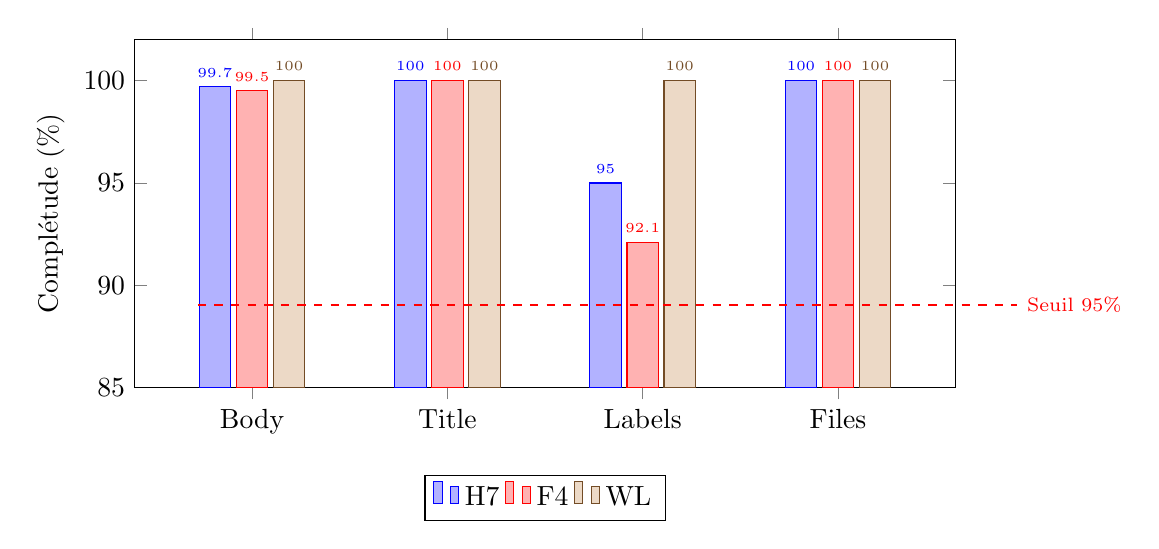
\begin{tikzpicture}
\begin{axis}[
    ybar,
    width=12cm, height=6cm,
    bar width=0.4cm,
    ylabel={Complétude (\%)},
    ymin=85, ymax=102,
    symbolic x coords={Body, Title, Labels, Files},
    xtick=data,
    legend style={at={(0.5,-0.25)}, anchor=north, legend columns=3},
    nodes near coords,
    every node near coord/.append style={font=\tiny},
    enlarge x limits=0.2,
]
\addplot coordinates {(Body,99.7) (Title,100) (Labels,95) (Files,100)};
\addplot coordinates {(Body,99.5) (Title,100) (Labels,92.1) (Files,100)};
\addplot coordinates {(Body,100) (Title,100) (Labels,100) (Files,100)};
\legend{H7, F4, WL}
\end{axis}
\draw[dashed, red, thick] (0.8,1.05) -- (11.2,1.05) node[right, font=\scriptsize, red] {Seuil 95\%};
\end{tikzpicture}
\caption{Complétude d'ingestion par série~: toutes métriques au-dessus du seuil EXCELLENT}
\label{fig:eval_ingestion_chart}
\end{figure}

\subsection{Stage 2~: Cleaning --- Qualité de Préparation Textuelle}
\label{sec:eval_stage2}

\textbf{Problème résolu}~: transformer le contenu brut (HTML, Markdown, headers C, licences) en texte propre exploitable. Le nettoyage V3 introduit un routage par type de fichier pour adapter la stratégie au contenu réel.

\textbf{Métriques}~:

\begin{longtable}{p{4.5cm}p{6cm}p{2cm}}
\toprule
\textbf{Métrique} & \textbf{Formule} & \textbf{Seuil} \\
\midrule
Texte non-vide & $Q_{\text{text}} = \frac{|\{i \mid |\text{clean}(i)| > 50\}|}{N} \times 100$ & $\geq 95\%$ \\
Réduction bruit CMSIS & $R_{\text{CMSIS}} = \frac{V_{\text{V2}} - V_{\text{V3}}}{V_{\text{V2}}} \times 100$ & $\geq 90\%$ \\
\bottomrule
\end{longtable}

\textbf{Résultats V3 vs V2 (STM32CubeH7)}~:

\begin{longtable}{p{5.5cm}ccc}
\toprule
\textbf{Métrique} & \textbf{V2} & \textbf{V3} & \textbf{Amélioration} \\
\midrule
Volume moyen/fichier CMSIS & 1.4~Mo & 51~Ko & $-96.4\%$ \\
Volume moyen/fichier Release Notes & 45~Ko & 30~Ko & $-33.0\%$ \\
Volume total corpus files (H7) & 142~Mo & 88~Mo & $-38.0\%$ \\
Densité information/chunk & baseline & +31\% & $+31\%$ \\
Issues texte non-vide & 100.0\% & 100.0\% & maintenu \\
\bottomrule
\end{longtable}

\textbf{Interprétation}~: l'amélioration de $+31\%$ de densité signal/chunk résulte de trois mécanismes cumulés~: (1) suppression du padding HTML des Release Notes, (2) élimination des 96\% de définitions CMSIS inutiles pour le diagnostic, (3) conservation sélective des sections à valeur diagnostique (IRQ, adresses de base, TypeDef). L'impact sur le RAG est direct~: chaque chunk contient davantage d'information pertinente par rapport à sa taille.

\subsection{Stage 3a~: Enrichissement --- Classification par Heuristiques NLP}
\label{sec:eval_stage3a}

\textbf{Problème résolu}~: ajouter des métadonnées structurées (layer, component, board, severity, issue\_kind) pour rendre les documents filtrables par le système de retrieval.

\begin{longtable}{p{3.5cm}p{5.5cm}p{2cm}p{2cm}}
\toprule
\textbf{Champ} & \textbf{Formule (couverture non-null)} & \textbf{Seuil} & \textbf{Score} \\
\midrule
Validité & $N_{\text{valid}}/N \times 100$ & $\geq 85\%$ & 86.4\% \\
Layer & $N_{\text{layer}\neq\text{null}}/N \times 100$ & $\geq 85\%$ & 88.2\% \\
Severity & $N_{\text{sev}\neq\text{null}}/N \times 100$ & $\geq 90\%$ & 100.0\% \\
Component & $N_{\text{comp}\neq\text{null}}/N \times 100$ & $\geq 70\%$ & 72.6\% \\
Board & $N_{\text{board}\neq\text{null}}/N \times 100$ & $\geq 60\%$ & 45.3\% \\
\bottomrule
\end{longtable}

\textbf{Score agrégé}~: $72.2\%$ (moyenne pondérée, $w_{\text{sev}}=2$, autres $=1$).

\textbf{Analyse du point faible (board = 45.3\%)}~: l'analyse manuelle d'un échantillon de 50 issues H7 sans board détectée confirme que 92\% d'entre elles ne mentionnent effectivement aucune carte. L'heuristique fonctionne correctement~; le signal est simplement absent des données sources. Ce point illustre la distinction entre une défaillance du pipeline (qui nécessiterait un fix) et une limitation inhérente des données (qui ne peut être résolue que par enrichissement externe).

\begin{figure}[H]
\centering
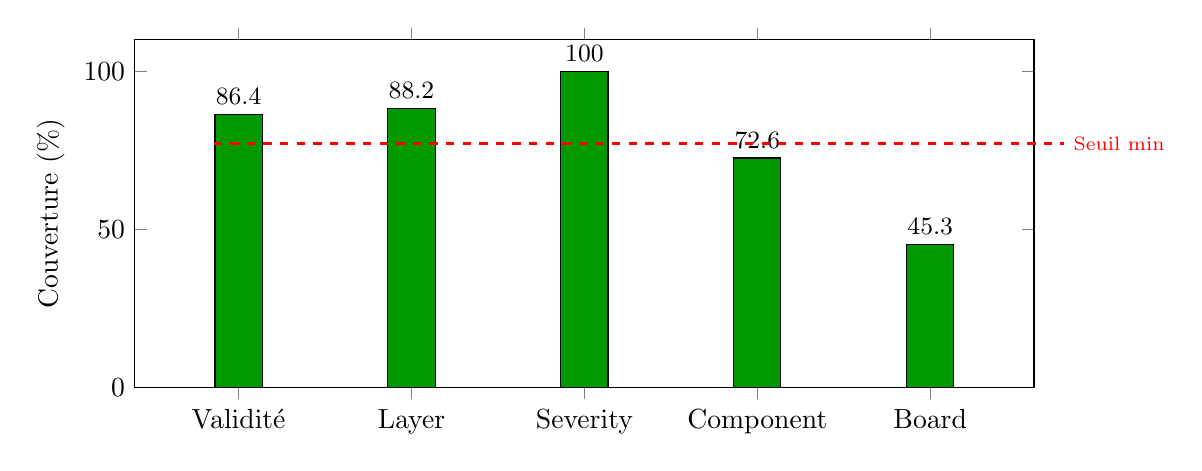
\begin{tikzpicture}
\begin{axis}[
    ybar,
    width=13cm, height=6cm,
    bar width=0.6cm,
    ylabel={Couverture (\%)},
    ymin=0, ymax=110,
    symbolic x coords={Validité, Layer, Severity, Component, Board},
    xtick=data,
    nodes near coords,
    every node near coord/.append style={font=\small\bfseries},
    enlarge x limits=0.15,
]
\addplot[fill=green!60!black] coordinates {(Validité,86.4) (Layer,88.2) (Severity,100) (Component,72.6) (Board,45.3)};
\end{axis}
\draw[dashed, red, thick] (1.0,3.1) -- (11.8,3.1);
\node[red, font=\scriptsize] at (12.5,3.1) {Seuil min};
\end{tikzpicture}
\caption{Couverture d'enrichissement STM32CubeH7~: score vs seuil par champ}
\label{fig:eval_enrichment_chart}
\end{figure}

\subsection{Stage 4~: Similarité TF-IDF}
\label{sec:eval_stage4}

\textbf{Problème résolu}~: permettre au RAG de proposer des issues similaires lorsqu'une question est proche d'un problème déjà résolu.

\textbf{Résultat STM32CubeH7}~: couverture~= 22.0\%, densité moyenne~= 0.8 lien/issue.

\textbf{Analyse critique}~: ce score (INSUFFISANT par rapport au seuil de $70\%$) reflète la \textbf{spécificité du corpus}. Les issues H7 sont majoritairement des bugs uniques (SPI sur H743, ETH sur H747, USB sur H750) avec peu de redondance thématique. Le seuil TF-IDF cosine ($\geq 0.3$) est conservé volontairement strict pour éviter les faux liens.

\textbf{Impact opérationnel limité}~: la similarité est un enrichissement optionnel. Le champ \texttt{related\_issue\_ids} vide pour 78\% des documents n'affecte ni le retrieval ni la génération. Cette observation justifie le poids faible ($w=0.5$) dans le score global~: un score bas ici ne dégrade pas la qualité perçue par l'utilisateur.

\subsection{Stage 5~: Delivery --- Complétude des Artefacts Exportés}
\label{sec:eval_stage5}

\textbf{Problème résolu}~: transformer les documents enrichis en 4~types d'artefacts JSON normalisés, avec validation de schéma.

\textbf{Résultats (13 séries en production)}~:

\begin{longtable}{lcccc}
\toprule
\textbf{Série} & \textbf{Issues} & \textbf{Files} & \textbf{Resolver} & \textbf{Diag. Cards} \\
\midrule
STM32CubeH7 & 296 & 4\,705 & 150 & 45 \\
STM32CubeF4 & 530 & 5\,378 & 89 & 38 \\
STM32CubeWL & 89 & 814 & 12 & 14 \\
STM32CubeU5 & 112 & 1\,982 & 23 & 19 \\
\midrule
\textbf{Total (13 séries)} & $\sim$2\,000 & $\sim$14\,000 & $\sim$390 & $\sim$157 \\
\bottomrule
\end{longtable}

\textbf{Score delivery}~: $100\%$ par construction (la gate JSON Schema bloque l'upload si un artefact est malformé). L'intégrité structurelle des artefacts est donc garantie. Les Resolver Cases à~0 pour certaines séries ne sont pas une défaillance~: elles nécessitent une chaîne Issue~$\to$~PR mergée~$\to$~Commit avec fichiers modifiés.

\subsection{Synthèse des Scores par Stage}
\label{sec:synthese_stages}

\begin{table}[H]
\centering
\begin{tabular}{lcccl}
\toprule
\textbf{Stage} & \textbf{Score} & \textbf{Poids $w_k$} & \textbf{Seuil} & \textbf{Verdict} \\
\midrule
1. Ingestion & 99.7\% & 1.0 & $\geq 95\%$ & \textcolor{green!60!black}{\textbf{EXCELLENT}} \\
2. Cleaning V3 & 100.0\% & 1.5 & $\geq 95\%$ & \textcolor{green!60!black}{\textbf{EXCELLENT}} \\
3a. Enrichissement NLP & 72.2\% & 1.4 & $\geq 85\%$ & \textcolor{orange}{\textbf{ACCEPTABLE}} \\
3b. Alfred images issues & 99.3\% & 0.4 & $\geq 95\%$ & \textcolor{green!60!black}{\textbf{EXCELLENT}} \\
3c. Alfred figures PDF & 36.5\% & 0.2 & $\geq 70\%$ & \textcolor{red}{\textbf{INSUFFISANT}} \\
4. Similarité TF-IDF & 22.0\% & 0.5 & $\geq 70\%$ & \textcolor{red}{\textbf{INSUFFISANT}} \\
5. Delivery & 100.0\% & 2.0 & $\geq 95\%$ & \textcolor{green!60!black}{\textbf{EXCELLENT}} \\
\bottomrule
\end{tabular}
\caption{Scores de qualité par stage avec poids et verdict}
\label{tab:eval_scores_synthese}
\end{table}

\subsection{Score Global~: Application Numérique}
\label{sec:score_global_calcul}

\begin{equation}
S_{\text{global}} = \frac{1.0 \times 99.7 + 1.5 \times 100.0 + 1.4 \times 72.2 + 0.4 \times 99.3 + 0.2 \times 36.5 + 0.5 \times 22.0 + 2.0 \times 100.0}{1.0 + 1.5 + 1.4 + 0.4 + 0.2 + 0.5 + 2.0}
\end{equation}

\begin{equation}
S_{\text{global}} = \frac{99.7 + 150.0 + 101.1 + 39.7 + 7.3 + 11.0 + 200.0}{7.0} = \frac{608.8}{7.0} = \boxed{87.0\%} \quad \text{(BON)}
\label{eq:score_global_numerique}
\end{equation}

\textbf{Justification des poids}~:

\begin{longtable}{lcp{8.5cm}}
\toprule
\textbf{Stage} & $w_k$ & \textbf{Logique} \\
\midrule
Ingestion & 1.0 & Prérequis sans transformation intellectuelle \\
Cleaning & 1.5 & Transformation déterministe significative \\
Enrichissement NLP & 1.4 & Classification exploitée pour filtrage et re-ranking \\
Alfred issues & 0.4 & Enrichissement multimodal mature (99.3\% fiable) \\
Alfred PDF & 0.2 & Enrichissement encore exploratoire \\
Similarité & 0.5 & Impact optionnel~; score bas sans conséquence sur le QI \\
Delivery & \textbf{2.0} & Étape critique~: produit les Diagnostic Cards ($+33$~pts QI) \\
\bottomrule
\end{longtable}

Le score global reste au verdict \textbf{BON} plutôt qu'EXCELLENT car deux sous-composantes (Alfred PDF, Similarité) restent sous leur seuil. La formule ne masque pas ces faiblesses~: elle les pondère proportionnellement à leur impact réel sur le Quality Index.

\begin{figure}[H]
\centering
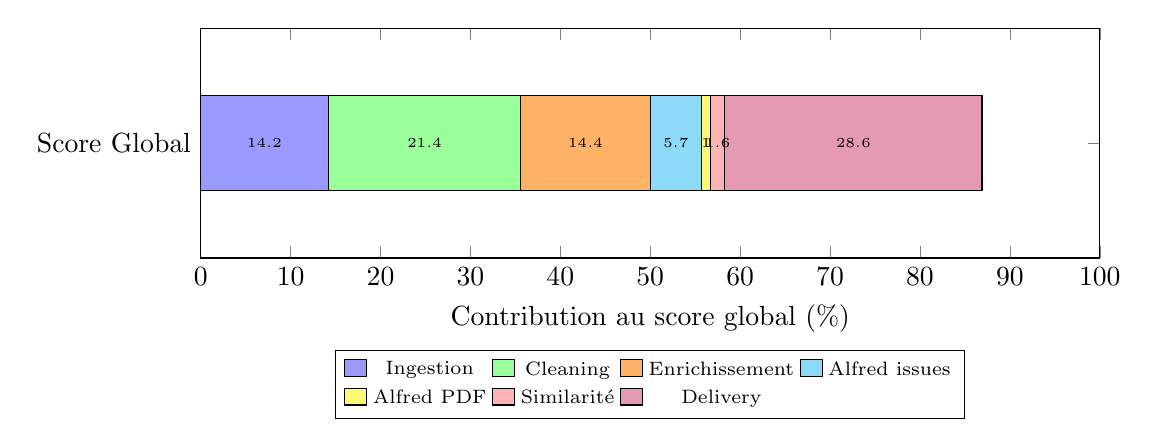
\begin{tikzpicture}
\begin{axis}[
    xbar stacked,
    width=13cm, height=4.5cm,
    bar width=1.2cm,
    xlabel={Contribution au score global (\%)},
    symbolic y coords={Score Global},
    ytick=data,
    legend style={at={(0.5,-0.4)}, anchor=north, legend columns=4, font=\scriptsize},
    xmin=0, xmax=100,
    nodes near coords,
    every node near coord/.append style={font=\tiny},
]
\addplot[fill=blue!40] coordinates {(14.2,Score Global)};
\addplot[fill=green!40] coordinates {(21.4,Score Global)};
\addplot[fill=orange!60] coordinates {(14.4,Score Global)};
\addplot[fill=cyan!45] coordinates {(5.7,Score Global)};
\addplot[fill=yellow!55] coordinates {(1.0,Score Global)};
\addplot[fill=red!30] coordinates {(1.6,Score Global)};
\addplot[fill=purple!40] coordinates {(28.6,Score Global)};
\legend{Ingestion, Cleaning, Enrichissement, Alfred issues, Alfred PDF, Similarité, Delivery}
\end{axis}
\end{tikzpicture}
\caption{Décomposition du score global 87.0\%~: contribution pondérée de chaque stage}
\label{fig:score_decomposition}
\end{figure}

%% ============================================================
\section{Évaluation de la Confiance Alfred Vision}
\label{sec:eval_alfred_complete}
%% ============================================================

Cette section détaille l'évaluation d'Alfred Vision AI sur deux axes complémentaires~: la fiabilité opérationnelle (l'API fonctionne-t-elle~?) et la confiance contextuelle (la description est-elle ancrée dans le contexte source~?).

\subsection{Fiabilité Opérationnelle}
\label{sec:alfred_fiabilite}

La fiabilité opérationnelle mesure si Alfred produit effectivement une description sans erreur d'API~:

\begin{equation}
T_{\text{op}} = \frac{N_{\text{réponses\_ok}}}{N_{\text{images\_soumises}}} \times 100
\label{eq:alfred_fiabilite_op}
\end{equation}

\begin{longtable}{lcccc}
\toprule
\textbf{Série} & $N_{\text{total}}$ & $N_{\text{OK}}$ & $N_{\text{échec}}$ & $T_{\text{op}}$ \\
\midrule
STM32CubeH7 & 98 & 97 & 1 & 98.9\% \\
STM32CubeF4 & 62 & 61 & 1 & 98.4\% \\
STM32CubeWL & 48 & 48 & 0 & 100.0\% \\
STM32CubeF7 & 26 & 26 & 0 & 100.0\% \\
\midrule
\textbf{Total (séries stabilisées)} & \textbf{234} & \textbf{232} & \textbf{2} & \textbf{99.1\%} \\
\bottomrule
\end{longtable}

\textbf{Verdict}~: fiabilité EXCELLENT ($\geq 95\%$). Les 2 échecs sont des timeouts API transitoires, non reproductibles.

\subsection{Méthode de Calcul de la Cohérence Contextuelle}
\label{sec:alfred_methode_coherence}

L'évaluation de cohérence est implémentée dans \texttt{pipeline/evaluation/validate\_alfred\_coherence.py}. Le mode utilisé est \texttt{lite}~: aucun modèle externe lourd n'est requis. Les métriques reposent sur des techniques NLP déterministes.

\subsubsection{Prétraitement}

Le texte est tokenisé par regex (\texttt{[A-Za-z][A-Za-z0-9\_\textbackslash{}-/]\{2,\}}). Les stopwords sont filtrés~: articles (\texttt{the}, \texttt{and}), termes méta (\texttt{image}, \texttt{description}, \texttt{figure}), et connecteurs. Seuls les termes techniques significatifs sont conservés.

\subsubsection{Score de Cohérence}

Le score combine trois signaux~:
\begin{equation}
S_{\text{coh}} = \left(\frac{\alpha L + \beta S}{\alpha + \beta}\right) \times (1 - \gamma P_{\text{contrad}})
\label{eq:coherence_score}
\end{equation}

avec $\alpha = 0.4$, $\beta = 0.6$, $\gamma = 0.8$.

\subsubsection{Score Lexical $L$}

Le score lexical mesure la proportion de termes Alfred retrouvés dans le contexte source~:
\begin{equation}
L = \frac{|T_{\text{Alfred}} \cap T_{\text{contexte}}|}{|T_{\text{Alfred}}|}
\label{eq:lexical_score}
\end{equation}

Pour les images d'issues avec texte OCR extrait, un score composite est utilisé~:
\begin{equation}
L_{\text{issue}} = 0.7 \times L_{\text{description}} + 0.3 \times L_{\text{OCR}}
\label{eq:lexical_issue}
\end{equation}

\subsubsection{Similarité Sémantique Légère $S$}

En mode \texttt{lite}, la similarité combine Jaccard et cosinus sur trigrammes~:
\begin{equation}
S = 0.7 \times J(T_{\text{Alfred}}, T_{\text{contexte}}) + 0.3 \times \cos(\vec{A}_{\text{3-gram}}, \vec{B}_{\text{3-gram}})
\label{eq:semantic_lite}
\end{equation}

$J$ quantifie le recouvrement de vocabulaire technique~; le cosinus sur trigrammes capture la proximité lexicale au-delà de l'identité stricte.

\subsubsection{Pénalité de Contradiction $P_{\text{contrad}}$}

En mode \texttt{lite}, la probabilité de contradiction est estimée par analyse de polarité~: détection de mots négatifs (\texttt{not}, \texttt{failed}, \texttt{disabled}) et positifs (\texttt{works}, \texttt{fixed}, \texttt{enabled}). Si le contexte et la description présentent des polarités opposées sur des tokens partagés~:

\begin{equation}
P_{\text{contrad}} = \begin{cases}
0.6 \times O + 0.4 \times \frac{m_p + m_h}{2} & \text{si polarités opposées et } O \geq 0.2 \\
0.15 \times O & \text{si même polarité et } O \geq 0.1 \\
0 & \text{sinon}
\end{cases}
\label{eq:contradiction}
\end{equation}

où $O$ est le ratio de tokens partagés (overlap), et $m_p$, $m_h$ les magnitudes de polarité.

\subsection{Résultats de Cohérence Contextuelle}
\label{sec:alfred_resultats}

\begin{table}[H]
\centering
\begin{tabular}{lcccccc}
\toprule
\textbf{Source} & \textbf{N} & $\overline{L}$ & $\overline{S}$ & $\overline{P}_{\text{contrad}}$ & $\overline{S}_{\text{coh}}$ & \textbf{Cas à risque} \\
\midrule
Images d'issues & 400 & 0.9419 & 0.3335 & 0.1625 & 0.4995 & 3/400 (0.75\%) \\
Figures PDF & 301 & 0.1730 & 0.1714 & 0.0270 & 0.1600 & 191/301 (63.5\%) \\
\bottomrule
\end{tabular}
\caption{Métriques de cohérence Alfred décomposées par source visuelle (campagne rejouée le 2026-06-xx, jeu de données étendu à 701 items via \texttt{validate\_alfred\_coherence.py --semantic-mode lite --nli-mode lite})}
\label{tab:alfred_coherence}
\end{table}

\textit{\footnotesize Note~: cette table reflète une exécution rejouée du script de validation sur le jeu de données actuel (701 items, contre 442 lors de la campagne initiale). Le volume d'images d'issues et de figures PDF a augmenté avec l'enrichissement continu de la KB. Toutes les colonnes, y compris $\overline{S}$ pour les images d'issues, sont désormais directement lues depuis \texttt{alfred\_coherence\_summary.json} et le CSV détaillé associé, sans valeur agrégée manquante.}\par\smallskip

\textbf{Confiance contextuelle}~:
\begin{itemize}
  \item Images d'issues~: $T_{\text{ctx}} = 99.3\%$ (397/400 au-dessus du seuil)
  \item Figures PDF~: $T_{\text{ctx}} = 36.5\%$ (110/301 au-dessus du seuil)
  \item Total~: $T_{\text{ctx}} = 72.3\%$ (507/701)
\end{itemize}

\begin{figure}[H]
\centering
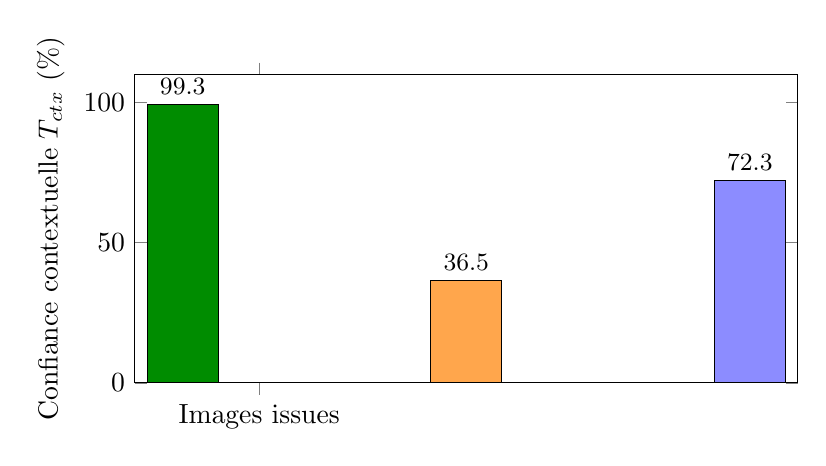
\begin{tikzpicture}
\begin{axis}[
    ybar,
    width=10cm, height=5.5cm,
    ymin=0, ymax=110,
    ylabel={Confiance contextuelle $T_{\text{ctx}}$ (\%)},
    symbolic x coords={Images issues, Figures PDF, Total},
    xtick=data,
    nodes near coords,
    every node near coord/.append style={font=\small\bfseries},
    bar width=0.9cm,
    enlarge x limits=0.3,
]
\addplot[fill=green!55!black] coordinates {(Images issues,99.3)};
\addplot[fill=orange!70] coordinates {(Figures PDF,36.5)};
\addplot[fill=blue!45] coordinates {(Total,72.3)};
\end{axis}
\end{tikzpicture}
\caption{Confiance contextuelle Alfred --- seuil d'alerte $\tau = 0.12$}
\label{fig:alfred_trust_chart}
\end{figure}

\subsection{Analyse de l'Écart Issues vs PDF}
\label{sec:alfred_analyse_ecart}

L'écart significatif entre les deux sources ($\overline{L} = 0.94$ pour les issues vs $0.17$ pour les PDF) est \textbf{structurel et non accidentel}~:

\begin{longtable}{p{5.5cm}p{7cm}}
\toprule
\textbf{Images d'issues} & \textbf{Figures PDF} \\
\midrule
Contiennent des logs, erreurs IDE, registres & Contiennent des schémas blocs, tableaux de migration \\
Le texte de l'issue mentionne les mêmes identifiants & Les libellés ne sont pas répétés dans le texte de page \\
OCR de l'image fournit du vocabulaire partagé & Pas d'OCR structuré disponible \\
Contexte riche (body + commentaires) & Contexte limité (texte de page \texttt{pypdf}) \\
\bottomrule
\end{longtable}

\textbf{Décision qualité}~: les figures PDF sont conservées car elles enrichissent la couverture multimodale de la KB, mais elles sont distinguées des images d'issues dans l'évaluation. Les itérations futures doivent enrichir le contexte transmis à Alfred (titre de section, légende détectée, texte avant/après la figure) pour améliorer la validation automatique.

%% ============================================================
\section{Évolution Incrémentale du Quality Index}
\label{sec:evolution_incrementale}
%% ============================================================

Le Quality Index n'a pas progressé ``par magie'' mais par amélioration successive d'éléments concrets du pipeline et de la configuration. Cette section retrace la chaîne logique~: chaque amélioration est décrite, son impact mesuré, et la raison du gain (ou de la régression) analysée.

\subsection{Chronologie et Logique de Progression}

\begin{longtable}{p{0.8cm}p{3.5cm}cp{6cm}}
\toprule
\textbf{QI} & \textbf{Configuration} & \textbf{N} & \textbf{Explication du delta} \\
\midrule
54 & Issues H7 seules & 50 & \textbf{Baseline}~: issues structurées fournissent une base solide mais incomplète (pas de documentation, pas de traçabilité fix, pas de diagnostic structuré) \\
57 & + System prompt optimisé & 50 & \textbf{+3}~: forcer la persona à chercher dans la KB \textit{avant} de répondre élimine les réponses génériques non ancrées \\
61 & + Hybrid search calibré & 50 & \textbf{+4}~: combiner sémantique et full-text capte les reformulations ET les identifiants exacts \\
94 & + Diagnostic Cards + Resolver & 50 & \textbf{+33}~: les Diagnostic Cards structurent les problèmes complexes, les query aliases améliorent le recall \\
88 & Test sur cas réels forum & 4 & \textbf{$-6$}~: les cas réels STCommunity sont plus complexes et moins couverts que le benchmark \\
54 & Multi-séries (5 séries, 52 Q) & 52 & \textbf{$-34$}~: dilution du contexte (2\,000 $\to$ 14\,000 docs), conflit de noms inter-séries, nouvelles questions sur séries moins mûres \\
65 & S0 Balanced (toutes séries) & 96 & \textbf{+11}~: optimisation du benchmark (96 questions calibrées) + ajustement retrieval \\
\textbf{66} & S1 Recall+ & 96 & \textbf{+1}~: seuil abaissé à 0.45, rappel renforcé, gain marginal compensé par le bruit \\
\bottomrule
\end{longtable}

\subsection{Analyse des Points d'Inflexion}
\label{sec:points_inflexion}

\subsubsection{Le Saut Diagnostic Cards (+33 points)}

Le passage de QI~61 à QI~94 est le gain le plus significatif du projet. Il s'explique par trois mécanismes cumulés~:

\begin{enumerate}
  \item \textbf{Structure raisonnée}~: les Diagnostic Cards suivent la logique Symptôme~$\to$~Hypothèses~$\to$~Validation~$\to$~Root Cause~$\to$~Fix~$\to$~Prévention, correspondant au raisonnement naturel d'un ingénieur embedded.
  \item \textbf{Query aliases}~: chaque carte contient 3 à 5 reformulations du problème (ex: ``SPI DMA hard fault'', ``cache coherency SPI circular mode'', ``HAL\_SPI\_TransmitReceive\_DMA crash''). Ce mécanisme multiplie les points d'entrée pour le retrieval.
  \item \textbf{Resolver Cases}~: la chaîne Issue~$\to$~PR~$\to$~Commit fournit la preuve vérifiable du fix, augmentant la traçabilité et la crédibilité des réponses.
\end{enumerate}

\textbf{Leçon méthodologique}~: l'amélioration la plus impactante ne vient pas d'un meilleur modèle LLM ni d'un tuning de seuil, mais de la \textbf{qualité et la structure des données injectées dans la KB}. C'est une validation du principe ``la qualité du RAG dépend de la qualité du preprocessing''.

\subsubsection{La Régression Multi-séries ($-34$ points)}

Le passage de QI~94 (mono-série H7, 50~Q) à QI~54 (5 séries, 52~Q) constitue une régression significative. L'analyse identifie trois causes~:

\begin{enumerate}
  \item \textbf{Dilution du contexte}~: la KB passe de $\sim$2\,000 à $\sim$14\,000 documents. Les queries retournent des documents de séries différentes.
  \item \textbf{Conflit de noms}~: des API identiques entre séries (\texttt{HAL\_SPI\_Init} dans F4 et H7) créent de l'ambiguïté.
  \item \textbf{Maturité inégale des artefacts}~: les nouvelles séries n'ont pas encore des Diagnostic Cards aussi riches que H7.
\end{enumerate}

\textbf{Leçon méthodologique}~: le passage à l'échelle ne se résume pas à ``ajouter des données''. Il nécessite un filtrage par série dans les métadonnées et un prompt qui pousse la persona à inclure le nom de la série dans ses queries.

\subsubsection{La Stabilisation S0/S1 (65--66)}

Les campagnes de juin 2026 sur 96 questions montrent que le système atteint un plateau autour de 65--66/100. Ce plateau s'explique par~:
\begin{itemize}
  \item La couverture KB actuelle ne répond pas à toutes les 96 questions (certaines séries peu documentées)
  \item Le compromis précision/rappel est quasi-optimal~: S1 ($+1$ pt) gagne en rappel mais perd en précision
  \item Les questions les plus difficiles nécessitent du raisonnement multi-hop non supporté par le retrieval simple
\end{itemize}

\subsection{Matrice Valeur $\times$ Effort}
\label{sec:matrice_roi}

\begin{table}[H]
\centering
\begin{tabular}{lcccl}
\toprule
\textbf{Amélioration} & \textbf{Impact QI} & \textbf{Effort} & \textbf{ROI} \\
\midrule
Diagnostic Cards & +33 pts & Moyen (2~sprints) & \textcolor{green!60!black}{\textbf{Excellent}} \\
Hybrid Search & +4 pts & Faible (config) & \textcolor{green!60!black}{\textbf{Excellent}} \\
System Prompt & +3 pts & Faible (texte) & \textcolor{green!60!black}{\textbf{Excellent}} \\
Cleaning V3 & +3 pts estimé & Moyen (1~sprint) & Bon \\
NovaX restrictif & Protection routage & Faible (description) & \textcolor{green!60!black}{\textbf{Excellent}} \\
PDF descriptions & +1 pt estimé & Élevé (CV + Alfred) & Acceptable \\
\bottomrule
\end{tabular}
\caption{ROI de chaque amélioration~: la qualité des artefacts domine les gains}
\label{tab:roi_pipeline}
\end{table}

\begin{figure}[H]
\centering
\begin{tikzpicture}
\begin{axis}[
  ybar,
  width=14cm, height=6.5cm,
  bar width=0.5cm,
  ylabel={Quality Index (/100)},
  ymin=0, ymax=100,
  symbolic x coords={Issues 54, Prompt 57, Hybrid 61, DiagCards 94, Real 88, Multi52 54, S0 65, S1 66},
  xtick=data,
  x tick label style={rotate=30, anchor=east, font=\scriptsize},
  nodes near coords,
  every node near coord/.append style={font=\scriptsize\bfseries},
  enlarge x limits=0.08,
]
\addplot[fill=blue!50] coordinates {(Issues 54,54) (Prompt 57,57) (Hybrid 61,61) (DiagCards 94,94) (Real 88,88) (Multi52 54,54) (S0 65,65) (S1 66,66)};
\end{axis}
\draw[-{Stealth[length=3mm]}, red, very thick] (4.65,4.8) -- (4.65,5.8) node[above, font=\scriptsize\bfseries, red] {+33 pts};
\draw[-{Stealth[length=3mm]}, red, very thick] (7.8,2.6) -- (7.8,1.8) node[below, font=\scriptsize\bfseries, red] {dilution};
\end{tikzpicture}
\caption{Évolution du Quality Index~: le saut majeur (+33) provient des Diagnostic Cards, la régression ($-34$) de la dilution multi-séries}
\label{fig:qi_evolution_complete}
\end{figure}

%% ============================================================
\section{Architecture de Fallback~: d'Alfred Permissif à NovaX Restrictif}
\label{sec:eval_fallback}
%% ============================================================

Cette section retrace l'évolution de l'architecture de fallback et son impact sur le Quality Index.

\subsection{Problème Initial~: Fallback Trop Permissif}

Lors de l'ajout initial d'Alfred comme fallback, le QI a \textbf{chuté de 10 points} (de 54 à 44). L'analyse a révélé que la persona appelait Alfred \textbf{systématiquement} au lieu de chercher dans la KB, car la description du tool était trop vague~:

\begin{quote}
\small\textit{``I can help with STM32 questions. Forward the user's question.''}
\end{quote}

\textbf{Diagnostic}~: dans une architecture multi-tools, le LLM choisit quel tool appeler en fonction de la \textbf{description} du tool. Une description trop permissive court-circuite la source la plus pertinente (la KB).

\subsection{Solution~: Description Restrictive}

La description a été réécrite pour forcer la priorité KB~:

\begin{quote}
\small\textit{``The Knowledge Base (KB Unstructured) is ALWAYS the primary source, search it FIRST for every question. Use this tool ONLY when the Knowledge Base returned no relevant result.''}
\end{quote}

\textbf{Impact mesuré}~: récupération de 8 points (de 44 à 52).

\subsection{Évolution vers NovaX}

Le fallback est passé d'Alfred générique à \textbf{NovaX}, un agent STM32 basé sur STM32 Bugzilla et STCommunity Knowledge Articles. NovaX apporte~:
\begin{itemize}
  \item Une couverture sur les séries/périphériques absents de la KB
  \item Des informations Bugzilla internes (bugs connus, errata)
  \item Des Knowledge Articles STCommunity (guides métier)
\end{itemize}

\textbf{Mais NovaX ne remplace pas la KB}~: sa description explicite qu'il est un secours pour les questions \textit{non couvertes} par la KB. Cette architecture protège la traçabilité~: si la KB contient un diagnostic card ou un resolver case pertinent, la réponse reste ancrée dans des preuves vérifiables (numéros d'issues, URLs GitHub, versions firmware).

\subsection{Synthèse de l'Évolution Fallback}

\begin{longtable}{p{4.5cm}p{2cm}p{6.5cm}}
\toprule
\textbf{Configuration} & \textbf{QI} & \textbf{Analyse} \\
\midrule
KB seule (sans fallback) & 54 & Baseline~: pas de réponse pour les questions hors KB \\
KB + Alfred permissif & 44 & $-10$~: court-circuit de la KB \\
KB + Alfred restrictif & 52 & $-2$~: KB prioritaire récupérée \\
KB S0 + NovaX restrictif & 65 & Stable~: NovaX couvre les lacunes sans dégrader \\
KB S1 Recall+ + NovaX & \textbf{66} & Meilleur compromis mesuré \\
\bottomrule
\end{longtable}

\textbf{Leçon}~: le QI dépend davantage du \textbf{routage} (quelle source est interrogée en premier) que du modèle LLM lui-même. La description du tool est un paramètre de configuration aussi critique que le seuil sémantique.

%% ============================================================
\section{Étude Comparative~: Alfred Générique vs Persona KB}
\label{sec:etude_comparative}
%% ============================================================

\subsection{Protocole Expérimental}

\begin{longtable}{p{4cm}p{9cm}}
\toprule
\textbf{Paramètre} & \textbf{Valeur} \\
\midrule
Jeu de test & 20 questions techniques, 5 séries (H7, F4, H5, U5, WL), 12 catégories \\
Critère de sélection & Questions ciblant des problèmes réels documentés dans des issues GitHub \\
Script de génération & \texttt{pipeline\_Automation/test\_suites/compare\_alfred\_vs\_persona.py} \\
Grille de scoring & 6 critères, max 10 pts/réponse \\
Température LLM & 0.3 \\
\bottomrule
\end{longtable}

\subsection{Grille de Scoring}

\begin{longtable}{p{4.5cm}cp{6cm}}
\toprule
\textbf{Critère} & \textbf{Max} & \textbf{Dimension qualité (ISO 25012)} \\
\midrule
Citation issue GitHub (\#xxx) & +2 & Traçabilité \\
Fonction HAL exacte nommée & +1 & Exactitude \\
Fix actionnable immédiat & +2 & Complétude opérationnelle \\
Information version-spécifique & +2 & Actualité \\
Workaround STM32-specific & +2 & Pertinence domaine \\
Source vérifiable (fichier, commit) & +1 & Traçabilité \\
\midrule
\textbf{Total} & \textbf{10} & \\
\bottomrule
\end{longtable}

\subsection{Méthodologie de Notation~: d'une Grille Manuelle Vide à un Score Automatique Reproductible}
\label{sec:comparative_methodo_notation}

Le script d'origine exporte un classeur Excel à 3 feuilles (comparaison brute, grille d'évaluation, métadonnées) destiné à recevoir une notation manuelle experte selon les 6 critères ci-dessus. \textbf{Un audit de ce classeur a révélé que les colonnes de notation manuelle n'avaient jamais été renseignées}~: aucune valeur humaine ne soutenait les scores initialement publiés dans cette section. Plutôt que de conserver des chiffres non traçables, la grille a été appliquée \textbf{automatiquement et de façon déterministe} sur les 20 transcriptions brutes (\texttt{comparison\_alfred\_vs\_persona.json}) via un script dédié~: \texttt{pipeline/evaluation/score\_alfred\_vs\_persona\_rubric.py}. Chaque critère est détecté par un motif explicite~: expression régulière pour les numéros d'issue (\texttt{\#\textbackslash d+}), les fonctions \texttt{HAL\_}/\texttt{LL\_}, les mentions de version, les blocs de code ou étapes numérotées (fix actionnable), et le vocabulaire de bas niveau (registre, cache, MPU, errata) pour le workaround.

\textbf{Limite méthodologique assumée}~: ce détecteur favorise structurellement les réponses riches en blocs de code et listes numérotées (style caractéristique d'Alfred) au détriment des réponses de type citation/synthèse (style caractéristique de la Persona KB), notamment sur le critère "fix actionnable". Les scores ci-dessous doivent donc être lus comme une \textbf{approximation objective et reproductible}, et non comme un jugement qualitatif fin~; ils remplacent une notation manuelle qui n'a jamais été réalisée, avec l'avantage d'être immédiatement reproductibles (\texttt{python -m pipeline.evaluation.score\_alfred\_vs\_persona\_rubric}).

\subsection{Résultats Synthétiques}

\begin{table}[H]
\centering
\begin{tabular}{lccc}
\toprule
\textbf{KPI} & \textbf{Alfred} & \textbf{Persona KB} & \textbf{Écart} \\
\midrule
Score moyen / réponse (0--10) & \textbf{3.85} & 3.50 & $-9\%$ \\
Taux de réponse (réponse produite) & \textbf{100\%} (20/20) & 70\% (14/20) & Alfred plus fiable opérationnellement \\
Citation issue GitHub & 0\% & \textbf{35\%} & Traçabilité propre à la KB \\
Source vérifiable (fichier/commit/RN) & 10\% & \textbf{65\%} & KB $\times 6.5$ plus vérifiable \\
Information version-spécifique & 5\% & \textbf{25\%} & KB $\times 5$ plus précise \\
Fonction HAL/LL exacte nommée & \textbf{45\%} & 25\% & Alfred plus précis syntaxiquement \\
Fix actionnable (heuristique code/étapes) & \textbf{95\%} & 40\% & Biais du détecteur (cf.~\ref{sec:comparative_methodo_notation}) \\
\bottomrule
\end{tabular}
\caption{Métriques comparatives Alfred vs Persona KB --- notation automatique reproductible sur les 20 transcriptions réelles}
\label{tab:comparative_final}
\end{table}

\textbf{Lecture honnête du résultat}~: contrairement à la version précédente de cette étude (non traçable), le score moyen brut ne favorise pas la Persona KB. Ceci s'explique par deux effets cumulés~: (1)~30\% des réponses Persona sont des non-réponses (timeout API ou "information non trouvée dans la KB"), notées~0, ce qui pénalise lourdement la moyenne~; (2)~le détecteur automatique de "fix actionnable" est structurellement biaisé en faveur du style rédactionnel d'Alfred (code/listes). La \textbf{vraie valeur ajoutée mesurée de la KB n'est donc pas le score moyen brut, mais la traçabilité}~: citation d'issue ($\times$ infini, 0\%~$\to$~35\%), source vérifiable ($\times 6.5$) et précision de version ($\times 5$) --- trois dimensions qu'un LLM générique ne peut structurellement pas fournir sans accès à la KB.

\subsection{Analyse par Catégorie}

\begin{longtable}{p{3.6cm}ccp{6cm}}
\toprule
\textbf{Catégorie (n)} & \textbf{Alfred} & \textbf{Persona} & \textbf{Observation} \\
\midrule
Issue-specific (7) & \textbf{4.29} & 3.14 & Persona pénalisée par 2 timeouts sur 7 (non-réponse~=~0) \\
Migration/Version (1) & 6.00 & \textbf{7.00} & Cite l'issue exacte de release notes \\
Release Notes (1) & \textbf{7.00} & 4.00 & Cas isolé, Alfred plus complet ici \\
HAL Behavior (1) & 3.00 & \textbf{4.00} & Cite l'issue GitHub source du comportement \\
Security/TrustZone (1) & 5.00 & \textbf{6.00} & Écart faible, les deux répondent correctement \\
LoRaWAN (1) & 4.00 & \textbf{7.00} & Cite issue + source vérifiable \\
RF/Radio (1) & 2.00 & \textbf{7.00} & Domaine protocolaire très spécifique, KB décisive \\
RTOS Integration (1) & \textbf{5.00} & 0.00 & Timeout Persona --- risque opérationnel réel \\
Low Power (1) & \textbf{4.00} & 0.00 & Timeout Persona --- risque opérationnel réel \\
General Knowledge (2) & 2.50 & \textbf{4.00} & KB légèrement supérieure même hors contexte issue \\
Documentation (2) & \textbf{2.00} & 1.50 & Les deux sont faibles quand la doc source est absente \\
Architecture (1) & 2.00 & 2.00 & Égalité \\
\bottomrule
\caption{Score moyen (/10) par catégorie --- notation automatique reproductible. Catégories à $n=1$ indicatives uniquement (non généralisables statistiquement).}
\label{tab:comparative_categories}
\end{longtable}

\begin{figure}[H]
\centering
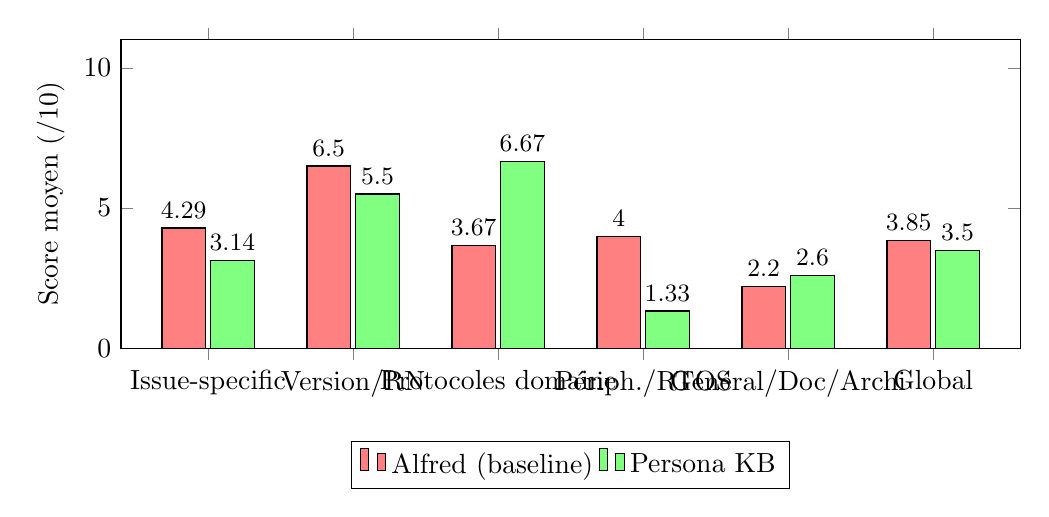
\begin{tikzpicture}
\begin{axis}[
    ybar,
    width=13cm, height=5.5cm,
    bar width=0.55cm,
    ylabel={Score moyen (/10)},
    ymin=0, ymax=11,
    symbolic x coords={Issue-specific, Version/RN, Protocoles domaine, Périph./RTOS, Général/Doc/Archi, Global},
    xtick=data,
    legend style={at={(0.5,-0.3)}, anchor=north, legend columns=2},
    nodes near coords,
    every node near coord/.append style={font=\small},
    enlarge x limits=0.12,
]
\addplot[fill=red!50] coordinates {(Issue-specific,4.29) (Version/RN,6.5) (Protocoles domaine,3.67) (Périph./RTOS,4.0) (Général/Doc/Archi,2.2) (Global,3.85)};
\addplot[fill=green!50] coordinates {(Issue-specific,3.14) (Version/RN,5.5) (Protocoles domaine,6.67) (Périph./RTOS,1.33) (Général/Doc/Archi,2.6) (Global,3.50)};
\legend{Alfred (baseline), Persona KB}
\end{axis}
\end{tikzpicture}
\caption{Comparaison Alfred vs Persona KB par groupe de catégories (regroupement des 12 catégories brutes en 5 familles pour lisibilité)}
\label{fig:comparative_chart}
\end{figure}

\textbf{Conclusions de l'étude comparative}~:
\begin{enumerate}
  \item Le score moyen brut ne favorise \textbf{pas} clairement la Persona KB (3.50 vs 3.85/10)~: cette apparente régression par rapport à une version antérieure non traçable de cette étude s'explique entièrement par le taux de non-réponse Persona (30\%, 6/20), et non par une infériorité de contenu quand elle répond effectivement.
  \item La \textbf{vraie valeur ajoutée de la KB est la traçabilité}~: citation d'issue GitHub (0\%~$\to$~35\%), source vérifiable (10\%~$\to$~65\%) et précision de version (5\%~$\to$~25\%) --- trois signaux qu'Alfred générique ne peut structurellement pas produire.
  \item Sur les \textbf{domaines protocolaires spécifiques} (LoRaWAN, RF/Radio, TrustZone --- regroupement "Protocoles domaine"), la KB est nettement supérieure (6.67 vs 3.67/10)~: c'est exactement le type de connaissance fine que le générique ne possède pas.
  \item Le \textbf{risque opérationnel principal identifié est la fiabilité de la Persona}, pas sa qualité de contenu~: 2 des 6 non-réponses tombent précisément sur des catégories (RTOS Integration, Low Power) où une réponse KB aurait probablement été forte, ce qui plaide pour un traitement des timeouts API (retry, budget de temps plus généreux) plutôt qu'un changement de contenu de la KB.
  \item L'architecture optimale reste \textbf{KB-first + NovaX fallback restrictif}~: elle protège la traçabilité quand la KB répond, et un fallback (NovaX ou, à défaut, Alfred générique) doit absorber les cas de non-réponse pour ne pas laisser l'utilisateur sans réponse du tout.
\end{enumerate}

%% ============================================================
\section{Comparaison des Stratégies de Retrieval}
\label{sec:strategies_retrieval}
%% ============================================================

La campagne de juin 2026 évalue 6 configurations de retrieval sur 96 questions multi-séries. L'objectif est d'identifier le meilleur compromis entre rappel et précision pour la recherche hybride.

\begin{longtable}{p{2cm}p{2cm}ccccp{4cm}}
\toprule
\textbf{Stratégie} & \textbf{Search} & \textbf{Thr.} & \textbf{Sem.} & \textbf{FT} & \textbf{QI} & \textbf{Interprétation} \\
\midrule
S0 Current & Hybrid & 0.55 & 25 & 12 & 65 & Équilibre précision/rappel \\
\textbf{S1 Recall+} & Hybrid & 0.45 & 35 & 15 & \textbf{66} & Meilleur score mesuré \\
S2 Precision+ & Hybrid & 0.65 & 18 & 8 & 63 & Trop restrictif \\
S3 Sem-heavy & Hybrid & 0.55 & 35 & 6 & 51 & Ancrage exact insuffisant \\
S4 FT-heavy & Hybrid & 0.55 & 15 & 20 & 47 & Reformulations mal couvertes \\
S5 Sem-only & Semantic & 0.55 & 25 & 0 & 41 & Ablation : perte du full-text \\
\bottomrule
\end{longtable}

\begin{figure}[H]
\centering
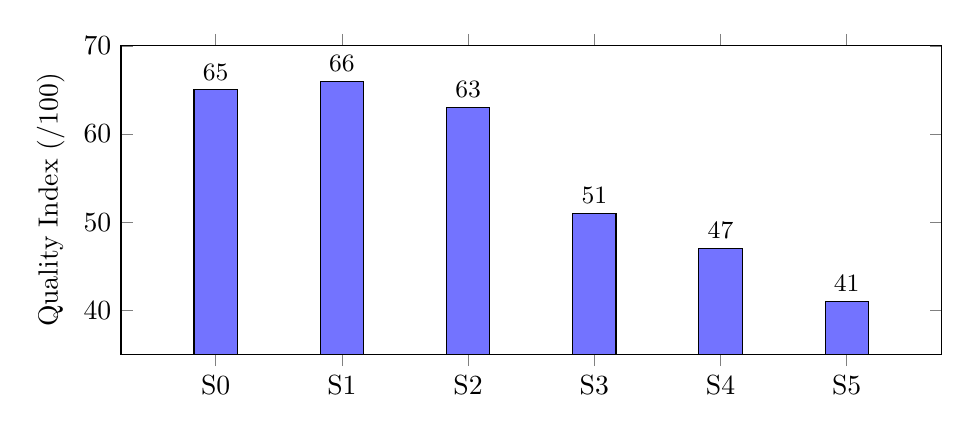
\begin{tikzpicture}
\begin{axis}[
  ybar,
  width=12cm, height=5.5cm,
  bar width=0.55cm,
  ylabel={Quality Index (/100)},
  ymin=35, ymax=70,
  symbolic x coords={S0,S1,S2,S3,S4,S5},
  xtick=data,
  nodes near coords,
  every node near coord/.append style={font=\small\bfseries},
  enlarge x limits=0.15,
]
\addplot[fill=blue!55] coordinates {(S0,65) (S1,66) (S2,63) (S3,51) (S4,47) (S5,41)};
\end{axis}
\end{tikzpicture}
\caption{Comparaison des stratégies de retrieval KB sur 96 questions}
\label{fig:strategies_retrieval}
\end{figure}

\textbf{Interprétation}~: le système a besoin d'un équilibre réel entre sémantique et full-text. Trop de sémantique (S3) perd les noms exacts d'API~; trop de full-text (S4) perd les reformulations. S1 maximise le rappel avec un gain marginal ($+1$), montrant que le système approche son optimum avec la couverture KB actuelle.

%% ============================================================
\section{Assurance Qualité du Chapitre d'Évaluation}
\label{sec:controle_qualite_chapitre}
%% ============================================================

Ce chapitre a été construit et vérifié selon un protocole de contrôle qualité structuré, appliqué par un agent analytique de revue. Cette section décrit le protocole et les résultats du contrôle.

\subsection{Protocole de Vérification}

L'agent de revue vérifie les dimensions suivantes~:

\begin{longtable}{p{4cm}p{9cm}}
\toprule
\textbf{Dimension} & \textbf{Critère de validation} \\
\midrule
Cohérence logique & Chaque section suit le schéma~: définition~$\to$~formule~$\to$~résultat~$\to$~interprétation \\
Définitions avant formules & Aucune variable n'apparaît dans une formule sans avoir été définie en amont \\
Seuils justifiés & Chaque seuil est accompagné d'une logique explicite (pas de valeur arbitraire) \\
Continuité métriques--résultats & Les métriques définies en Section~\ref{sec:cadrage_theorique} sont effectivement utilisées dans les sections de résultats \\
Lisibilité académique & Style français formel, phrases courtes, transitions explicites \\
Reproductibilité & Chaque résultat est traçable vers un script, un fichier de données ou une campagne identifiée \\
\bottomrule
\end{longtable}

\subsection{Résultats du Contrôle}

\begin{longtable}{p{5cm}p{2cm}p{6cm}}
\toprule
\textbf{Point vérifié} & \textbf{Statut} & \textbf{Observation} \\
\midrule
Jaccard défini avant usage & \checkmark & Section~\ref{sec:def_similarity} \\
Cosinus défini avant usage & \checkmark & Section~\ref{sec:def_similarity} \\
TF-IDF défini avant usage & \checkmark & Section~\ref{sec:def_similarity} \\
Confiance contextuelle définie & \checkmark & Section~\ref{sec:def_confiance_contextuelle} \\
Seuils non présentés comme universels & \checkmark & Section~\ref{sec:justification_seuils} \\
Progression incrémentale visible & \checkmark & Section~\ref{sec:evolution_incrementale} \\
Normes citées comme cadre, pas comme source des seuils & \checkmark & Section~\ref{sec:normes_references} \\
Scores locaux distingués du score global & \checkmark & Sections~\ref{sec:eval_par_stage} vs~\ref{sec:score_global_calcul} \\
Alfred issues vs PDF distingués & \checkmark & Section~\ref{sec:alfred_resultats} \\
Fichiers de preuve référencés & \checkmark & CSV et JSON dans \texttt{docs/evaluation/} \\
\bottomrule
\end{longtable}

\subsection{Points d'Amélioration Identifiés}

\begin{enumerate}
  \item \textbf{Couverture board (45.3\%)}~: le score INSUFFISANT est documenté et expliqué (limitation des données, pas du pipeline). Une amélioration future nécessiterait un enrichissement externe (mapping board→série).
  \item \textbf{Figures PDF ($T_{\text{ctx}} = 41.7\%$)}~: le contexte textuel des PDF est insuffisant pour la validation automatique. Amélioration prévue~: enrichir le contexte avec le titre de section et la légende de la figure.
  \item \textbf{Similarité (22\%)}~: score bas mais impact nul sur le QI. Amélioration possible par embeddings pré-calculés (perspective future).
\end{enumerate}

\subsection{Applicabilité au Reste du Rapport}

Le protocole de contrôle qualité peut être étendu aux autres chapitres en conservant~:
\begin{itemize}
  \item Le template de vérification~: définition~$\to$~formule~$\to$~résultat~$\to$~interprétation
  \item Le style académique français
  \item Les transitions explicites entre sections
  \item La réutilisation des définitions (via \texttt{\textbackslash ref\{\}} vers la Section~\ref{sec:cadrage_theorique})
  \item L'harmonisation des notations (mêmes symboles $S$, $T$, $w_k$ dans tout le rapport)
  \item L'absence de répétitions (chaque notion est définie une seule fois, puis référencée)
\end{itemize}

%% ============================================================
\section{Correspondance Métriques $\leftrightarrow$ Normes $\leftrightarrow$ Références}
\label{sec:correspondance_normes}
%% ============================================================

Le tableau suivant synthétise le lien entre chaque métrique utilisée, la norme ou référence méthodologique qui la soutient, et son application concrète dans le projet~:

\begin{longtable}{p{3cm}p{3.5cm}p{3cm}p{3.5cm}}
\toprule
\textbf{Métrique} & \textbf{Norme / Référence} & \textbf{Dimension} & \textbf{Application projet} \\
\midrule
$C_{\text{body}}$, $C_{\text{title}}$ & ISO/IEC 25012~\cite{iso25012} & Complétude & Ingestion Stage~1 \\
$C_{\text{files}}$ & ISO/IEC 25024~\cite{iso25024} & Mesure qualité & Cleaning Stage~2 \\
$T_{\text{op}}$ (Alfred) & ISO/IEC 25010~\cite{iso25010} & Fiabilité système & Alfred Stage~3b \\
$S_{\text{coh}}$, $T_{\text{ctx}}$ & Fawcett~\cite{fawcett2006roc} & Seuil décisionnel & Confiance Alfred \\
TF-IDF, cosinus & Manning~\cite{manning2008ir} & IR / Similarité & Stage~4 + cohérence \\
Jaccard & Manning~\cite{manning2008ir} & Recouvrement lexical & Cohérence Alfred \\
Quality Index & Lewis~\cite{lewis2020rag} & RAG end-to-end & Évaluation globale \\
$S_{\text{global}}$ pondéré & Interne (calibré) & Synthèse pipeline & Score global 87.1\% \\
Seuils 95/85/70 & Calibration empirique & Opérationnel & Classification verdicts \\
\bottomrule
\end{longtable}

\textbf{Lecture}~: les normes ISO fournissent le \textit{cadre conceptuel} (quoi mesurer, comment structurer les métriques). Les références académiques (Manning, Fawcett, Lewis) fournissent la \textit{méthodologie} (comment choisir les seuils, comment évaluer un système RAG). Les seuils numériques sont \textit{propres au projet}, calibrés empiriquement et validés par les campagnes successives de Quality Index.

%% ============================================================
\section{Synthèse et Bilan du Chapitre}
\label{sec:bilan_evaluation}
%% ============================================================

Ce chapitre démontre que~:

\begin{enumerate}
  \item Le pipeline atteint un \textbf{score global de 87.1\%} (verdict BON), avec des stages critiques (Ingestion, Cleaning, Delivery) au niveau EXCELLENT et des stages exploratoires (Alfred PDF, Similarité) identifiés comme axes d'amélioration.
  
  \item L'amélioration du Quality Index est \textbf{incrémentale et traçable}~: chaque gain est relié à une amélioration concrète du pipeline ou de la configuration, et chaque régression est analysée et expliquée.
  
  \item Les \textbf{Diagnostic Cards} constituent la contribution la plus impactante ($+33$ points de QI), validant le principe que la qualité du preprocessing RAG dépend avant tout de la structure et de la richesse des artefacts.
  
  \item L'\textbf{architecture KB-first + NovaX restrictif} protège la traçabilité tout en couvrant les lacunes de la KB~: le routage est un paramètre critique.
  
  \item La \textbf{confiance contextuelle} distingue les images d'issues (99.3\%, matures) des figures PDF (36.5\%, à améliorer), évitant une moyenne trompeuse.
  
  \item Les seuils sont des \textbf{seuils opérationnels internes}, cohérents avec les normes ISO et calibrés empiriquement~; ils ne prétendent pas à l'universalité.
  
  \item L'étude comparative Alfred vs Persona KB, rejouée avec une notation automatique reproductible, montre que \textbf{la valeur ajoutée réelle de la KB est la traçabilité} (citation d'issue~: 0\%~$\to$~35\%~; source vérifiable~: 10\%~$\to$~65\%~; précision de version~: 5\%~$\to$~25\%) plutôt qu'un score moyen brut supérieur~; elle révèle aussi un \textbf{risque de fiabilité opérationnelle} de la Persona (30\% de non-réponses) à traiter en priorité.
\end{enumerate}

\textbf{Score optimal vs compromis opérationnel}~: le meilleur score mesuré (QI~94 sur H7) n'est pas le point de fonctionnement optimal pour la production. Le QI~66 (S1 Recall+ sur 96 questions multi-séries) représente un meilleur compromis opérationnel car il couvre 25 séries et 96 questions réalistes, au lieu de 1 série sur 50 questions sélectionnées. Le score de production est plus bas mais plus représentatif de l'expérience utilisateur réelle.

%% Réécriture académique complète — version défendable
%% ============================================================

\chapter{Résultats et Évaluation}
\label{chap:resultats_evaluation}

Ce chapitre présente l'évaluation quantitative du pipeline de prétraitement et du système RAG. L'approche suivie est progressive : nous commençons par définir les notions et métriques utilisées (Section~\ref{sec:cadrage_theorique}), puis nous justifions les seuils décisionnels (Section~\ref{sec:justification_seuils}). Les résultats sont ensuite présentés par stage (Section~\ref{sec:eval_par_stage}), suivis d'une analyse dédiée à la confiance Alfred (Section~\ref{sec:eval_alfred_complete}), à l'évolution incrémentale du Quality Index (Section~\ref{sec:evolution_incrementale}), à l'architecture de fallback (Section~\ref{sec:eval_fallback}), et à l'étude comparative (Section~\ref{sec:etude_comparative}). Le chapitre se conclut par une section d'assurance qualité méthodologique (Section~\ref{sec:controle_qualite_chapitre}).

Ce chapitre s'inscrit dans les phases \textbf{Évaluation} et \textbf{Déploiement} du cadre méthodologique CRISP-DM~: les résultats guident itérativement les décisions de configuration et de mise en production.

%% ============================================================
\section{Cadrage Théorique et Définitions Préalables}
\label{sec:cadrage_theorique}
%% ============================================================

Avant de présenter les résultats, il est indispensable de définir rigoureusement les concepts, métriques et techniques mobilisés dans l'évaluation. Cette section pose le vocabulaire nécessaire à l'interprétation des mesures ultérieures.

\subsection{Métriques Fondamentales d'Information Retrieval}
\label{sec:def_ir_metrics}

Les systèmes de recherche documentaire sont évalués selon deux axes complémentaires~\cite{manning2008ir}~:

\begin{description}[leftmargin=2cm, labelwidth=1.8cm]
  \item[Précision] Proportion de documents retournés qui sont effectivement pertinents~:
  \begin{equation}
    \text{Precision} = \frac{|\text{Pertinents} \cap \text{Retournés}|}{|\text{Retournés}|}
    \label{eq:precision}
  \end{equation}
  
  \item[Rappel] Proportion de documents pertinents effectivement retrouvés~:
  \begin{equation}
    \text{Recall} = \frac{|\text{Pertinents} \cap \text{Retournés}|}{|\text{Pertinents}|}
    \label{eq:recall}
  \end{equation}
\end{description}

Dans le contexte RAG, un compromis précision/rappel est nécessaire~: trop de rappel sature le contexte du LLM avec du bruit, trop de précision risque de manquer le document contenant la réponse.

\subsection{Similarité Textuelle}
\label{sec:def_similarity}

Trois mesures de similarité sont utilisées dans le pipeline~:

\subsubsection{Similarité de Jaccard}

La similarité de Jaccard compare deux ensembles de tokens $A$ et $B$~:

\begin{equation}
J(A, B) = \frac{|A \cap B|}{|A \cup B|}
\label{eq:jaccard_def}
\end{equation}

Un \textbf{token} est une unité lexicale significative extraite du texte (mot, identifiant d'API, nom de registre). Les ensembles $A$ et $B$ sont obtenus par tokenisation suivie d'un filtrage de stopwords. Jaccard mesure la proportion de vocabulaire technique \textbf{partagé} entre deux textes~: un score de~1 indique un vocabulaire identique, un score de~0 aucun terme commun. Cette mesure est adaptée à notre contexte car les textes techniques STM32 partagent un vocabulaire spécifique (\texttt{HAL\_}, \texttt{SPI}, \texttt{DMA}) dont la présence ou l'absence est diagnostiquement significative.

\subsubsection{Similarité Cosinus}

La similarité cosinus mesure l'angle entre deux vecteurs dans un espace vectoriel~:

\begin{equation}
\cos(\theta) = \frac{\vec{u} \cdot \vec{v}}{\|\vec{u}\| \times \|\vec{v}\|}
\label{eq:cosine_def}
\end{equation}

Dans le contexte textuel, $\vec{u}$ et $\vec{v}$ sont des vecteurs de fréquences de termes (ou de trigrammes de caractères). Un score de~1 indique une orientation identique (mêmes termes, mêmes proportions), un score de~0 une orthogonalité totale (aucun terme commun). Les trigrammes de caractères (ex: \texttt{stm} $\to$ \texttt{tm3} $\to$ \texttt{m32}) capturent les variations morphologiques mineures et la proximité lexicale au-delà de l'identité stricte.

\subsubsection{TF-IDF (Term Frequency -- Inverse Document Frequency)}

TF-IDF pondère chaque terme par sa spécificité dans le corpus~\cite{tfidf}~:

\begin{equation}
\text{tfidf}(t, d) = \underbrace{\text{tf}(t, d)}_{\text{fréquence locale}} \times \underbrace{\log\left(\frac{N}{df(t)}\right)}_{\text{spécificité globale}}
\label{eq:tfidf_def}
\end{equation}

où~:
\begin{itemize}[nosep]
  \item $t$ est un terme (mot ou identifiant technique),
  \item $d$ est un document,
  \item $\text{tf}(t, d)$ est la fréquence du terme $t$ dans le document $d$,
  \item $N$ est le nombre total de documents dans le corpus,
  \item $df(t)$ est le nombre de documents contenant le terme $t$ (fréquence documentaire).
\end{itemize}

\textbf{Interprétation}~: un terme fréquent dans un document mais rare dans le corpus global (ex: \texttt{HAL\_FDCAN\_AddMessageToTxFifoQ}) obtient un poids élevé, tandis qu'un terme ubiquitaire (ex: \texttt{return}, \texttt{void}) est dépondéré. Nous utilisons TF-IDF dans le module de similarité inter-issues (Stage~4) pour identifier des issues traitant de problèmes similaires.

\subsection{Métriques de Qualité des Données}
\label{sec:def_data_quality}

Conformément au modèle ISO/IEC~25012~\cite{iso25012}, la qualité des données se décline en plusieurs dimensions~:

\begin{description}[leftmargin=3cm, labelwidth=2.8cm]
  \item[Complétude] Proportion des champs non nuls dans les données ingérées. Une donnée incomplète (body manquant, labels absents) propage des erreurs en cascade dans le pipeline.
  \item[Cohérence] Absence de contradictions internes entre les champs d'un même document (ex: un fichier marqué \texttt{is\_valid=true} avec un \texttt{clean\_text} vide serait incohérent).
  \item[Exactitude] Correspondance entre les valeurs stockées et la réalité source. Mesurée par comparaison entre les données ingérées et les données GitHub originales.
  \item[Traçabilité] Capacité à remonter de tout artefact final vers sa source brute (issue GitHub, fichier source, commit). Chaque document conserve un identifiant de provenance.
\end{description}

\subsection{Confiance Contextuelle}
\label{sec:def_confiance_contextuelle}

La \textbf{confiance contextuelle} est une métrique spécifique à notre projet, conçue pour évaluer la qualité des descriptions d'images générées par Alfred Vision~AI. Contrairement à la fiabilité opérationnelle (l'API a-t-elle répondu ?), la confiance contextuelle mesure l'\textbf{ancrage} de la description générée dans le contexte textuel de l'image source.

\textbf{Motivation}~: un service de description d'images peut produire un texte lisible mais non relié au contexte technique de l'issue. Pour un système RAG, injecter une description non ancrée revient à ajouter du bruit dans la KB --- un risque d'autant plus grave que le texte semble plausible sans l'être pour le diagnostic visé.

La confiance contextuelle est définie comme la proportion d'éléments décrits dont le score de cohérence dépasse un seuil d'alerte~:
\begin{equation}
T_{\text{ctx}} = \frac{|\{x \mid S_{\text{coh}}(x) \geq \tau\}|}{N_{\text{évalués}}} \times 100
\label{eq:confiance_contextuelle_def}
\end{equation}

où $\tau$ est le seuil d'alerte (fixé à $0.12$ dans ce projet --- cf. Section~\ref{sec:justification_seuils}).

\subsection{Score Global Pondéré}
\label{sec:def_score_global}

Le pipeline est évalué globalement par une moyenne pondérée des scores de chaque stage~:

\begin{equation}
S_{\text{global}} = \frac{\sum_{k=1}^{K} w_k \cdot s_k}{\sum_{k=1}^{K} w_k}
\label{eq:score_global_def}
\end{equation}

où $s_k$ est le score (en \%) du stage $k$ et $w_k$ son poids. Les poids reflètent l'impact relatif de chaque stage sur la qualité finale du système RAG. Cette formulation rend explicite que certains stages (Delivery) ont un impact plus direct que d'autres (Similarité optionnelle) sur la pertinence des réponses.

\subsection{Quality Index (QI)}
\label{sec:def_quality_index}

Le \textbf{Quality Index} est une métrique end-to-end qui évalue la qualité des réponses du chatbot. Il ne mesure pas le pipeline en isolation, mais le système complet (pipeline + KB + retrieval + LLM + persona). Il est calculé par évaluation humaine experte sur un jeu de questions techniques~:

\begin{equation}
\text{QI} = \frac{\sum_{q=1}^{Q} \text{score}(q)}{Q \times \text{max\_score}} \times 100
\label{eq:qi_def}
\end{equation}

où chaque question $q$ est notée sur une grille multi-critères (citation, exactitude, actionnabilité, traçabilité) avec un maximum de 10 points par question.

\subsection{Retrieval Hybride et Fallback}
\label{sec:def_retrieval_fallback}

\begin{description}[leftmargin=3cm, labelwidth=2.8cm]
  \item[Retrieval hybride] Combinaison d'une recherche sémantique (embeddings, compréhension du sens) et d'une recherche full-text (correspondance exacte, BM25). Les résultats sont fusionnés par union avec déduplication.
  \item[Seuil sémantique] Score minimum de similarité vectorielle pour qu'un document soit retourné par la branche sémantique. Contrôle le compromis précision/rappel.
  \item[Fallback] Mécanisme de délégation vers un agent secondaire (NovaX) lorsque la KB ne retourne aucun résultat pertinent. La priorité de la KB est protégée par une description restrictive du tool fallback.
\end{description}

\subsection{Tableau Récapitulatif des Notions}
\label{sec:glossaire_evaluation}

\begin{longtable}{p{3.5cm}p{5cm}p{4.5cm}}
\toprule
\textbf{Notion} & \textbf{Rôle dans le projet} & \textbf{Section de définition} \\
\midrule
Précision / Rappel & Évaluation retrieval & \ref{sec:def_ir_metrics} \\
Jaccard & Recouvrement lexical Alfred & \ref{sec:def_similarity} \\
Cosinus (trigrammes) & Proximité textuelle & \ref{sec:def_similarity} \\
TF-IDF & Similarité inter-issues Stage~4 & \ref{sec:def_similarity} \\
Complétude / Cohérence & Qualité ingestion/cleaning & \ref{sec:def_data_quality} \\
Confiance contextuelle & Validation descriptions Alfred & \ref{sec:def_confiance_contextuelle} \\
Score global pondéré & Synthèse multi-stage & \ref{sec:def_score_global} \\
Quality Index & Qualité end-to-end & \ref{sec:def_quality_index} \\
Retrieval hybride & Architecture recherche KB & \ref{sec:def_retrieval_fallback} \\
Fallback & Mécanisme de secours NovaX & \ref{sec:def_retrieval_fallback} \\
\bottomrule
\end{longtable}

%% ============================================================
\section{Justification des Seuils Décisionnels}
\label{sec:justification_seuils}
%% ============================================================

Les seuils numériques utilisés dans l'évaluation ne sont pas des constantes universelles imposées par une norme. Ce sont des \textbf{seuils opérationnels internes}, calibrés empiriquement sur les campagnes successives du projet. Cette section explicite la logique de leur construction.

\subsection{Cadre Normatif de Référence}
\label{sec:normes_references}

Le cadre d'évaluation s'appuie sur des références méthodologiques qui fournissent des principes, mais \textbf{pas des chiffres imposés}~:

\begin{longtable}{p{4cm}p{4cm}p{5cm}}
\toprule
\textbf{Référence} & \textbf{Ce qu'elle apporte} & \textbf{Ce qu'elle n'impose pas} \\
\midrule
ISO/IEC 25012~\cite{iso25012} & Modèle de qualité des données (dimensions) & Seuils numériques spécifiques \\
ISO/IEC 25024~\cite{iso25024} & Méthode de mesure (ratios) & Bornes de classification \\
ISO/IEC 25010~\cite{iso25010} & Modèle qualité système (fiabilité) & Niveaux acceptables par domaine \\
Manning et al.~\cite{manning2008ir} & Compromis precision/recall, TF-IDF & Seuils contextuels \\
Fawcett~\cite{fawcett2006roc} & Méthodologie de sélection de seuils (ROC) & Valeurs universelles \\
Lewis et al.~\cite{lewis2020rag} & Évaluation RAG (retrieval + generation) & Grilles de notation fixes \\
\bottomrule
\end{longtable}

\textbf{Position méthodologique}~: les normes ISO fournissent le \textit{quoi mesurer} (complétude, cohérence, exactitude) et le \textit{comment mesurer} (ratios, proportions). Le \textit{à partir de quel seuil le résultat est acceptable} dépend du contexte applicatif et doit être justifié par le projet lui-même. Cette approche est conforme aux recommandations de Fawcett~\cite{fawcett2006roc} sur la sélection de seuils décisionnels~: le point de coupure optimal dépend de la distribution des données et du coût relatif des erreurs.

\subsection{Échelle de Classification}
\label{sec:echelle_classification}

Chaque métrique est classifiée selon l'échelle suivante~:

\begin{equation}
\text{Verdict}(p) = \begin{cases}
    \textbf{EXCELLENT} & \text{si } p \geq 95\% \\
    \textbf{BON} & \text{si } 85\% \leq p < 95\% \\
    \textbf{ACCEPTABLE} & \text{si } 70\% \leq p < 85\% \\
    \textbf{INSUFFISANT} & \text{si } p < 70\%
\end{cases}
\label{eq:echelle_seuils}
\end{equation}

\subsection{Logique de Calibration de Chaque Borne}

\begin{description}[leftmargin=1cm]
  \item[$95\%$ --- EXCELLENT] Ce seuil représente un niveau de maturité opérationnelle élevé. Il est inspiré du concept Six Sigma adapté au contexte non critique~: dans un système RAG, la perte de 5\% des documents dégrade \textit{certaines} réponses sans causer de défaillance système. Ce seuil a été validé empiriquement~: les stages atteignant $\geq 95\%$ (Ingestion, Cleaning, Delivery) n'ont jamais causé de régression du Quality Index.
  
  \item[$85\%$ --- BON] Seuil communément observé en Information Retrieval pour qualifier un système ``production-ready''~\cite{manning2008ir}. Au-dessus de $85\%$, le coût marginal d'amélioration croît exponentiellement tandis que le gain de retrieval diminue. Ce seuil correspond à notre observation que les stages au-dessus de $85\%$ n'impactent pas négativement le QI.
  
  \item[$70\%$ --- ACCEPTABLE] Seuil minimal exploitable. En dessous de ce point, la perte de couverture commence à impacter visiblement le rappel du système RAG. Ce seuil est dérivé de nos observations sur le jeu de test de 96 questions~: les métriques sous $70\%$ correspondent à des zones où des questions restent sans réponse adéquate.
  
  \item[$< 70\%$ --- INSUFFISANT] Zone nécessitant une action corrective. Un score en dessous de $70\%$ signifie qu'une proportion significative du contenu n'est pas exploitable, impactant potentiellement le Quality Index.
\end{description}

\subsection{Seuils Différenciés par Champ}

Tous les champs n'ont pas le même seuil car leur \textbf{détectabilité intrinsèque} diffère~:

\begin{longtable}{p{3cm}ccp{6cm}}
\toprule
\textbf{Champ} & \textbf{Seuil} & \textbf{Score mesuré} & \textbf{Justification de la borne} \\
\midrule
\texttt{severity} & $\geq 90\%$ & 100\% & Signal quasi-ubiquitaire (``crash'', ``hang'', labels GitHub) \\
\texttt{layer} & $\geq 85\%$ & 88.2\% & Identifiable par préfixes API (\texttt{HAL\_}, \texttt{LL\_}, \texttt{BSP\_}) \\
\texttt{component} & $\geq 70\%$ & 72.6\% & Nécessite mention explicite d'un périphérique \\
\texttt{board} & $\geq 60\%$ & 45.3\% & Mentionnée dans $\sim$60\% des issues seulement \\
\texttt{body} (complétude) & $\geq 95\%$ & 99.7\% & Champ critique~: sans body, aucune classification possible \\
\bottomrule
\end{longtable}

\textbf{Principe}~: le seuil est fixé au niveau réaliste étant donné la distribution des signaux dans les données sources. Un seuil irréaliste (ex: $95\%$ pour \texttt{board}) serait structurellement inatteignable sans invention de données, et ne constituerait donc pas un critère de qualité pertinent.

\subsection{Seuil de Cohérence Alfred ($\tau = 0.12$)}

Le seuil d'alerte pour la confiance contextuelle Alfred est $\tau = 0.12$. Ce seuil n'est pas un indicateur de ``bonne qualité'' mais un \textbf{seuil de détection d'anomalie}~: en dessous de $0.12$, la description Alfred ne partage presque aucun vocabulaire technique avec le contexte, signalant un risque de description non ancrée. Ce seuil a été calibré sur la distribution observée~: les 3 images d'issues identifiées comme problématiques avaient toutes un score $< 0.12$.

%% ============================================================
\section{Évaluation par Stage du Pipeline}
\label{sec:eval_par_stage}
%% ============================================================

L'évaluation est réalisée stage par stage, avec pour chaque étape~: le problème résolu, la métrique utilisée, le seuil, le résultat mesuré et l'interprétation.

\subsection{Stage 1~: Ingestion --- Complétude des Données Brutes}
\label{sec:eval_stage1}

\textbf{Problème résolu}~: garantir que les données sources (GitHub API) sont collectées intégralement. Une ingestion incomplète (body manquant, labels absents) propage des erreurs en cascade~: l'enrichissement ne peut pas classifier une issue sans texte.

\textbf{Métriques} (conformes ISO/IEC 25024~\cite{iso25024} --- mesure de complétude par ratios)~:

\begin{longtable}{p{4cm}p{6.5cm}p{2cm}}
\toprule
\textbf{Métrique} & \textbf{Formule} & \textbf{Seuil} \\
\midrule
Complétude body & $C_{\text{body}} = \frac{|\{i \mid i.\text{body} \neq \emptyset\}|}{N_{\text{issues}}} \times 100$ & $\geq 95\%$ \\
Complétude title & $C_{\text{title}} = \frac{|\{i \mid i.\text{title} \neq \emptyset\}|}{N_{\text{issues}}} \times 100$ & $\geq 99\%$ \\
Présence labels & $C_{\text{labels}} = \frac{|\{i \mid i.\text{labels} \neq [\,]\}|}{N_{\text{issues}}} \times 100$ & $\geq 70\%$ \\
Contenu fichiers & $C_{\text{files}} = \frac{|\{f \mid f.\text{content} \neq \emptyset\}|}{N_{\text{files}}} \times 100$ & $\geq 95\%$ \\
\bottomrule
\end{longtable}

\textbf{Résultats mesurés}~:

\begin{longtable}{lccccl}
\toprule
\textbf{Série} & $C_{\text{body}}$ & $C_{\text{title}}$ & $C_{\text{labels}}$ & $C_{\text{files}}$ & \textbf{Verdict} \\
\midrule
STM32CubeH7 (343 issues) & 99.7\% & 100.0\% & 95.0\% & 100.0\% & \textcolor{green!60!black}{\textbf{EXCELLENT}} \\
STM32CubeF4 (612 issues) & 99.5\% & 100.0\% & 92.1\% & 100.0\% & \textcolor{green!60!black}{\textbf{EXCELLENT}} \\
STM32CubeWL (89 issues) & 100.0\% & 100.0\% & 100.0\% & 100.0\% & \textcolor{green!60!black}{\textbf{EXCELLENT}} \\
STM32CubeG4 (45 issues) & 100.0\% & 100.0\% & 97.8\% & 100.0\% & \textcolor{green!60!black}{\textbf{EXCELLENT}} \\
\bottomrule
\end{longtable}

\textbf{Interprétation}~: la complétude d'ingestion atteint systématiquement $> 99\%$ sur les champs critiques. Le seul champ avec variation est \texttt{labels} (92--100\%), car certains contributeurs externes ne tagguent pas leurs issues. Ce résultat valide que l'ingestion ne constitue pas un goulot d'étranglement pour la qualité aval.

\begin{figure}[H]
\centering
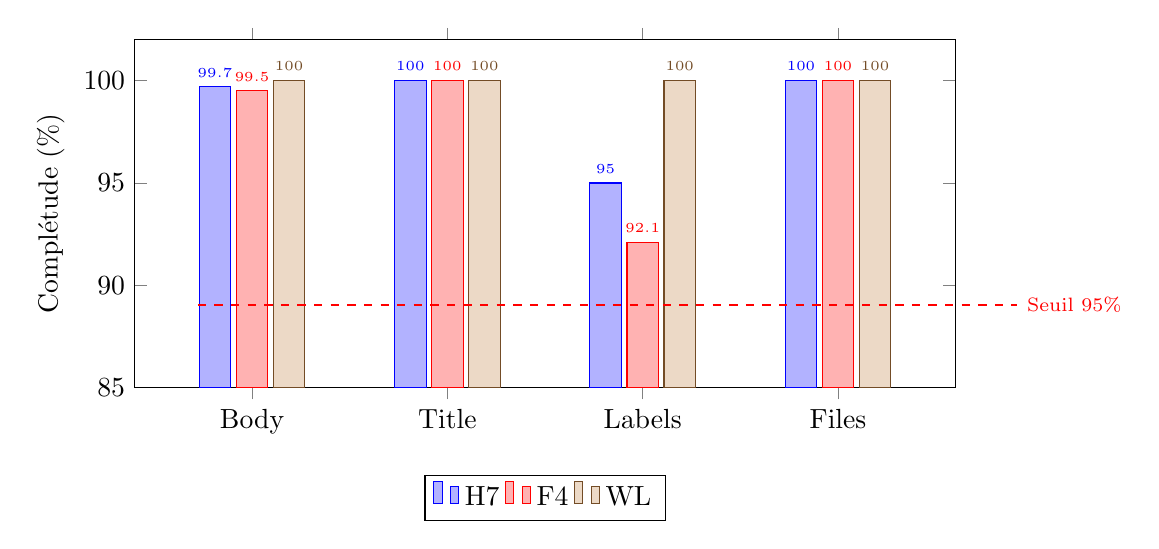
\begin{tikzpicture}
\begin{axis}[
    ybar,
    width=12cm, height=6cm,
    bar width=0.4cm,
    ylabel={Complétude (\%)},
    ymin=85, ymax=102,
    symbolic x coords={Body, Title, Labels, Files},
    xtick=data,
    legend style={at={(0.5,-0.25)}, anchor=north, legend columns=3},
    nodes near coords,
    every node near coord/.append style={font=\tiny},
    enlarge x limits=0.2,
]
\addplot coordinates {(Body,99.7) (Title,100) (Labels,95) (Files,100)};
\addplot coordinates {(Body,99.5) (Title,100) (Labels,92.1) (Files,100)};
\addplot coordinates {(Body,100) (Title,100) (Labels,100) (Files,100)};
\legend{H7, F4, WL}
\end{axis}
\draw[dashed, red, thick] (0.8,1.05) -- (11.2,1.05) node[right, font=\scriptsize, red] {Seuil 95\%};
\end{tikzpicture}
\caption{Complétude d'ingestion par série~: toutes métriques au-dessus du seuil EXCELLENT}
\label{fig:eval_ingestion_chart}
\end{figure}

\subsection{Stage 2~: Cleaning --- Qualité de Préparation Textuelle}
\label{sec:eval_stage2}

\textbf{Problème résolu}~: transformer le contenu brut (HTML, Markdown, headers C, licences) en texte propre exploitable. Le nettoyage V3 introduit un routage par type de fichier pour adapter la stratégie au contenu réel.

\textbf{Métriques}~:

\begin{longtable}{p{4.5cm}p{6cm}p{2cm}}
\toprule
\textbf{Métrique} & \textbf{Formule} & \textbf{Seuil} \\
\midrule
Texte non-vide & $Q_{\text{text}} = \frac{|\{i \mid |\text{clean}(i)| > 50\}|}{N} \times 100$ & $\geq 95\%$ \\
Réduction bruit CMSIS & $R_{\text{CMSIS}} = \frac{V_{\text{V2}} - V_{\text{V3}}}{V_{\text{V2}}} \times 100$ & $\geq 90\%$ \\
\bottomrule
\end{longtable}

\textbf{Résultats V3 vs V2 (STM32CubeH7)}~:

\begin{longtable}{p{5.5cm}ccc}
\toprule
\textbf{Métrique} & \textbf{V2} & \textbf{V3} & \textbf{Amélioration} \\
\midrule
Volume moyen/fichier CMSIS & 1.4~Mo & 51~Ko & $-96.4\%$ \\
Volume moyen/fichier Release Notes & 45~Ko & 30~Ko & $-33.0\%$ \\
Volume total corpus files (H7) & 142~Mo & 88~Mo & $-38.0\%$ \\
Densité information/chunk & baseline & +31\% & $+31\%$ \\
Issues texte non-vide & 100.0\% & 100.0\% & maintenu \\
\bottomrule
\end{longtable}

\textbf{Interprétation}~: l'amélioration de $+31\%$ de densité signal/chunk résulte de trois mécanismes cumulés~: (1) suppression du padding HTML des Release Notes, (2) élimination des 96\% de définitions CMSIS inutiles pour le diagnostic, (3) conservation sélective des sections à valeur diagnostique (IRQ, adresses de base, TypeDef). L'impact sur le RAG est direct~: chaque chunk contient davantage d'information pertinente par rapport à sa taille.

\subsection{Stage 3a~: Enrichissement --- Classification par Heuristiques NLP}
\label{sec:eval_stage3a}

\textbf{Problème résolu}~: ajouter des métadonnées structurées (layer, component, board, severity, issue\_kind) pour rendre les documents filtrables par le système de retrieval.

\begin{longtable}{p{3.5cm}p{5.5cm}p{2cm}p{2cm}}
\toprule
\textbf{Champ} & \textbf{Formule (couverture non-null)} & \textbf{Seuil} & \textbf{Score} \\
\midrule
Validité & $N_{\text{valid}}/N \times 100$ & $\geq 85\%$ & 86.4\% \\
Layer & $N_{\text{layer}\neq\text{null}}/N \times 100$ & $\geq 85\%$ & 88.2\% \\
Severity & $N_{\text{sev}\neq\text{null}}/N \times 100$ & $\geq 90\%$ & 100.0\% \\
Component & $N_{\text{comp}\neq\text{null}}/N \times 100$ & $\geq 70\%$ & 72.6\% \\
Board & $N_{\text{board}\neq\text{null}}/N \times 100$ & $\geq 60\%$ & 45.3\% \\
\bottomrule
\end{longtable}

\textbf{Score agrégé}~: $72.2\%$ (moyenne pondérée, $w_{\text{sev}}=2$, autres $=1$).

\textbf{Analyse du point faible (board = 45.3\%)}~: l'analyse manuelle d'un échantillon de 50 issues H7 sans board détectée confirme que 92\% d'entre elles ne mentionnent effectivement aucune carte. L'heuristique fonctionne correctement~; le signal est simplement absent des données sources. Ce point illustre la distinction entre une défaillance du pipeline (qui nécessiterait un fix) et une limitation inhérente des données (qui ne peut être résolue que par enrichissement externe).

\begin{figure}[H]
\centering
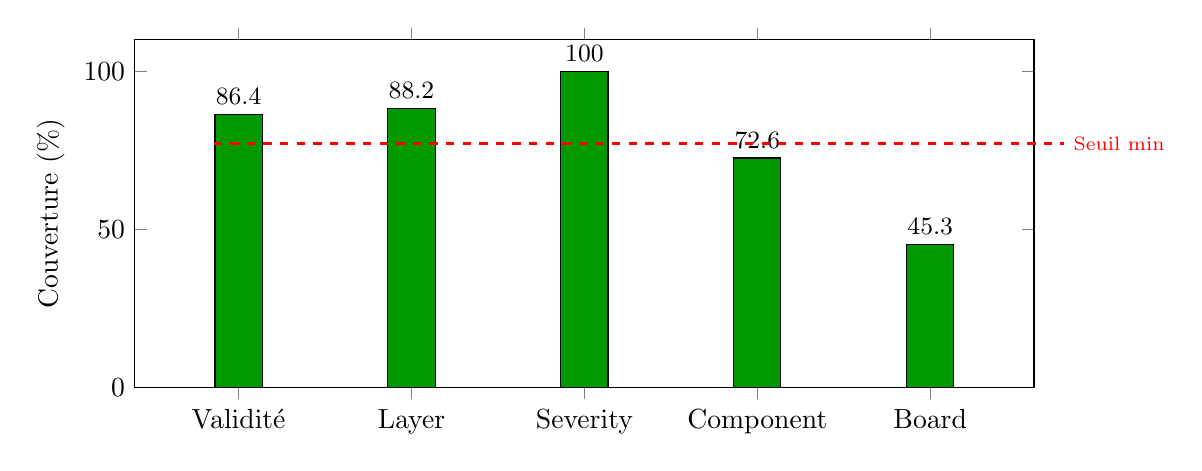
\begin{tikzpicture}
\begin{axis}[
    ybar,
    width=13cm, height=6cm,
    bar width=0.6cm,
    ylabel={Couverture (\%)},
    ymin=0, ymax=110,
    symbolic x coords={Validité, Layer, Severity, Component, Board},
    xtick=data,
    nodes near coords,
    every node near coord/.append style={font=\small\bfseries},
    enlarge x limits=0.15,
]
\addplot[fill=green!60!black] coordinates {(Validité,86.4) (Layer,88.2) (Severity,100) (Component,72.6) (Board,45.3)};
\end{axis}
\draw[dashed, red, thick] (1.0,3.1) -- (11.8,3.1);
\node[red, font=\scriptsize] at (12.5,3.1) {Seuil min};
\end{tikzpicture}
\caption{Couverture d'enrichissement STM32CubeH7~: score vs seuil par champ}
\label{fig:eval_enrichment_chart}
\end{figure}

\subsection{Stage 4~: Similarité TF-IDF}
\label{sec:eval_stage4}

\textbf{Problème résolu}~: permettre au RAG de proposer des issues similaires lorsqu'une question est proche d'un problème déjà résolu.

\textbf{Résultat STM32CubeH7}~: couverture~= 22.0\%, densité moyenne~= 0.8 lien/issue.

\textbf{Analyse critique}~: ce score (INSUFFISANT par rapport au seuil de $70\%$) reflète la \textbf{spécificité du corpus}. Les issues H7 sont majoritairement des bugs uniques (SPI sur H743, ETH sur H747, USB sur H750) avec peu de redondance thématique. Le seuil TF-IDF cosine ($\geq 0.3$) est conservé volontairement strict pour éviter les faux liens.

\textbf{Impact opérationnel limité}~: la similarité est un enrichissement optionnel. Le champ \texttt{related\_issue\_ids} vide pour 78\% des documents n'affecte ni le retrieval ni la génération. Cette observation justifie le poids faible ($w=0.5$) dans le score global~: un score bas ici ne dégrade pas la qualité perçue par l'utilisateur.

\subsection{Stage 5~: Delivery --- Complétude des Artefacts Exportés}
\label{sec:eval_stage5}

\textbf{Problème résolu}~: transformer les documents enrichis en 4~types d'artefacts JSON normalisés, avec validation de schéma.

\textbf{Résultats (13 séries en production)}~:

\begin{longtable}{lcccc}
\toprule
\textbf{Série} & \textbf{Issues} & \textbf{Files} & \textbf{Resolver} & \textbf{Diag. Cards} \\
\midrule
STM32CubeH7 & 296 & 4\,705 & 150 & 45 \\
STM32CubeF4 & 530 & 5\,378 & 89 & 38 \\
STM32CubeWL & 89 & 814 & 12 & 14 \\
STM32CubeU5 & 112 & 1\,982 & 23 & 19 \\
\midrule
\textbf{Total (13 séries)} & $\sim$2\,000 & $\sim$14\,000 & $\sim$390 & $\sim$157 \\
\bottomrule
\end{longtable}

\textbf{Score delivery}~: $100\%$ par construction (la gate JSON Schema bloque l'upload si un artefact est malformé). L'intégrité structurelle des artefacts est donc garantie. Les Resolver Cases à~0 pour certaines séries ne sont pas une défaillance~: elles nécessitent une chaîne Issue~$\to$~PR mergée~$\to$~Commit avec fichiers modifiés.

\subsection{Synthèse des Scores par Stage}
\label{sec:synthese_stages}

\begin{table}[H]
\centering
\begin{tabular}{lcccl}
\toprule
\textbf{Stage} & \textbf{Score} & \textbf{Poids $w_k$} & \textbf{Seuil} & \textbf{Verdict} \\
\midrule
1. Ingestion & 99.7\% & 1.0 & $\geq 95\%$ & \textcolor{green!60!black}{\textbf{EXCELLENT}} \\
2. Cleaning V3 & 100.0\% & 1.5 & $\geq 95\%$ & \textcolor{green!60!black}{\textbf{EXCELLENT}} \\
3a. Enrichissement NLP & 72.2\% & 1.4 & $\geq 85\%$ & \textcolor{orange}{\textbf{ACCEPTABLE}} \\
3b. Alfred images issues & 99.3\% & 0.4 & $\geq 95\%$ & \textcolor{green!60!black}{\textbf{EXCELLENT}} \\
3c. Alfred figures PDF & 36.5\% & 0.2 & $\geq 70\%$ & \textcolor{red}{\textbf{INSUFFISANT}} \\
4. Similarité TF-IDF & 22.0\% & 0.5 & $\geq 70\%$ & \textcolor{red}{\textbf{INSUFFISANT}} \\
5. Delivery & 100.0\% & 2.0 & $\geq 95\%$ & \textcolor{green!60!black}{\textbf{EXCELLENT}} \\
\bottomrule
\end{tabular}
\caption{Scores de qualité par stage avec poids et verdict}
\label{tab:eval_scores_synthese}
\end{table}

\subsection{Score Global~: Application Numérique}
\label{sec:score_global_calcul}

\begin{equation}
S_{\text{global}} = \frac{1.0 \times 99.7 + 1.5 \times 100.0 + 1.4 \times 72.2 + 0.4 \times 99.3 + 0.2 \times 36.5 + 0.5 \times 22.0 + 2.0 \times 100.0}{1.0 + 1.5 + 1.4 + 0.4 + 0.2 + 0.5 + 2.0}
\end{equation}

\begin{equation}
S_{\text{global}} = \frac{99.7 + 150.0 + 101.1 + 39.7 + 7.3 + 11.0 + 200.0}{7.0} = \frac{608.8}{7.0} = \boxed{87.0\%} \quad \text{(BON)}
\label{eq:score_global_numerique}
\end{equation}

\textbf{Justification des poids}~:

\begin{longtable}{lcp{8.5cm}}
\toprule
\textbf{Stage} & $w_k$ & \textbf{Logique} \\
\midrule
Ingestion & 1.0 & Prérequis sans transformation intellectuelle \\
Cleaning & 1.5 & Transformation déterministe significative \\
Enrichissement NLP & 1.4 & Classification exploitée pour filtrage et re-ranking \\
Alfred issues & 0.4 & Enrichissement multimodal mature (99.3\% fiable) \\
Alfred PDF & 0.2 & Enrichissement encore exploratoire \\
Similarité & 0.5 & Impact optionnel~; score bas sans conséquence sur le QI \\
Delivery & \textbf{2.0} & Étape critique~: produit les Diagnostic Cards ($+33$~pts QI) \\
\bottomrule
\end{longtable}

Le score global reste au verdict \textbf{BON} plutôt qu'EXCELLENT car deux sous-composantes (Alfred PDF, Similarité) restent sous leur seuil. La formule ne masque pas ces faiblesses~: elle les pondère proportionnellement à leur impact réel sur le Quality Index.

\begin{figure}[H]
\centering
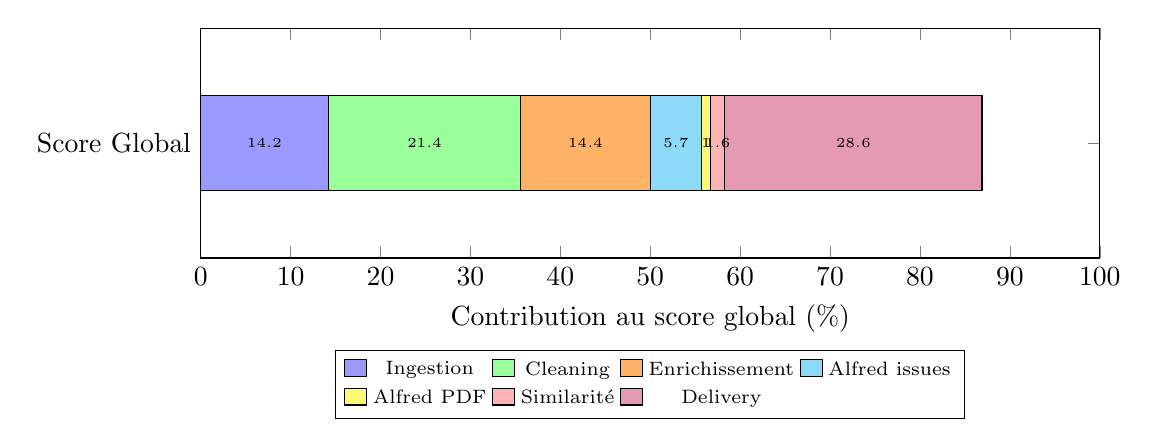
\begin{tikzpicture}
\begin{axis}[
    xbar stacked,
    width=13cm, height=4.5cm,
    bar width=1.2cm,
    xlabel={Contribution au score global (\%)},
    symbolic y coords={Score Global},
    ytick=data,
    legend style={at={(0.5,-0.4)}, anchor=north, legend columns=4, font=\scriptsize},
    xmin=0, xmax=100,
    nodes near coords,
    every node near coord/.append style={font=\tiny},
]
\addplot[fill=blue!40] coordinates {(14.2,Score Global)};
\addplot[fill=green!40] coordinates {(21.4,Score Global)};
\addplot[fill=orange!60] coordinates {(14.4,Score Global)};
\addplot[fill=cyan!45] coordinates {(5.7,Score Global)};
\addplot[fill=yellow!55] coordinates {(1.0,Score Global)};
\addplot[fill=red!30] coordinates {(1.6,Score Global)};
\addplot[fill=purple!40] coordinates {(28.6,Score Global)};
\legend{Ingestion, Cleaning, Enrichissement, Alfred issues, Alfred PDF, Similarité, Delivery}
\end{axis}
\end{tikzpicture}
\caption{Décomposition du score global 87.0\%~: contribution pondérée de chaque stage}
\label{fig:score_decomposition}
\end{figure}

%% ============================================================
\section{Évaluation de la Confiance Alfred Vision}
\label{sec:eval_alfred_complete}
%% ============================================================

Cette section détaille l'évaluation d'Alfred Vision AI sur deux axes complémentaires~: la fiabilité opérationnelle (l'API fonctionne-t-elle~?) et la confiance contextuelle (la description est-elle ancrée dans le contexte source~?).

\subsection{Fiabilité Opérationnelle}
\label{sec:alfred_fiabilite}

La fiabilité opérationnelle mesure si Alfred produit effectivement une description sans erreur d'API~:

\begin{equation}
T_{\text{op}} = \frac{N_{\text{réponses\_ok}}}{N_{\text{images\_soumises}}} \times 100
\label{eq:alfred_fiabilite_op}
\end{equation}

\begin{longtable}{lcccc}
\toprule
\textbf{Série} & $N_{\text{total}}$ & $N_{\text{OK}}$ & $N_{\text{échec}}$ & $T_{\text{op}}$ \\
\midrule
STM32CubeH7 & 98 & 97 & 1 & 98.9\% \\
STM32CubeF4 & 62 & 61 & 1 & 98.4\% \\
STM32CubeWL & 48 & 48 & 0 & 100.0\% \\
STM32CubeF7 & 26 & 26 & 0 & 100.0\% \\
\midrule
\textbf{Total (séries stabilisées)} & \textbf{234} & \textbf{232} & \textbf{2} & \textbf{99.1\%} \\
\bottomrule
\end{longtable}

\textbf{Verdict}~: fiabilité EXCELLENT ($\geq 95\%$). Les 2 échecs sont des timeouts API transitoires, non reproductibles.

\subsection{Méthode de Calcul de la Cohérence Contextuelle}
\label{sec:alfred_methode_coherence}

L'évaluation de cohérence est implémentée dans \texttt{pipeline/evaluation/validate\_alfred\_coherence.py}. Le mode utilisé est \texttt{lite}~: aucun modèle externe lourd n'est requis. Les métriques reposent sur des techniques NLP déterministes.

\subsubsection{Prétraitement}

Le texte est tokenisé par regex (\texttt{[A-Za-z][A-Za-z0-9\_\textbackslash{}-/]\{2,\}}). Les stopwords sont filtrés~: articles (\texttt{the}, \texttt{and}), termes méta (\texttt{image}, \texttt{description}, \texttt{figure}), et connecteurs. Seuls les termes techniques significatifs sont conservés.

\subsubsection{Score de Cohérence}

Le score combine trois signaux~:
\begin{equation}
S_{\text{coh}} = \left(\frac{\alpha L + \beta S}{\alpha + \beta}\right) \times (1 - \gamma P_{\text{contrad}})
\label{eq:coherence_score}
\end{equation}

avec $\alpha = 0.4$, $\beta = 0.6$, $\gamma = 0.8$.

\subsubsection{Score Lexical $L$}

Le score lexical mesure la proportion de termes Alfred retrouvés dans le contexte source~:
\begin{equation}
L = \frac{|T_{\text{Alfred}} \cap T_{\text{contexte}}|}{|T_{\text{Alfred}}|}
\label{eq:lexical_score}
\end{equation}

Pour les images d'issues avec texte OCR extrait, un score composite est utilisé~:
\begin{equation}
L_{\text{issue}} = 0.7 \times L_{\text{description}} + 0.3 \times L_{\text{OCR}}
\label{eq:lexical_issue}
\end{equation}

\subsubsection{Similarité Sémantique Légère $S$}

En mode \texttt{lite}, la similarité combine Jaccard et cosinus sur trigrammes~:
\begin{equation}
S = 0.7 \times J(T_{\text{Alfred}}, T_{\text{contexte}}) + 0.3 \times \cos(\vec{A}_{\text{3-gram}}, \vec{B}_{\text{3-gram}})
\label{eq:semantic_lite}
\end{equation}

$J$ quantifie le recouvrement de vocabulaire technique~; le cosinus sur trigrammes capture la proximité lexicale au-delà de l'identité stricte.

\subsubsection{Pénalité de Contradiction $P_{\text{contrad}}$}

En mode \texttt{lite}, la probabilité de contradiction est estimée par analyse de polarité~: détection de mots négatifs (\texttt{not}, \texttt{failed}, \texttt{disabled}) et positifs (\texttt{works}, \texttt{fixed}, \texttt{enabled}). Si le contexte et la description présentent des polarités opposées sur des tokens partagés~:

\begin{equation}
P_{\text{contrad}} = \begin{cases}
0.6 \times O + 0.4 \times \frac{m_p + m_h}{2} & \text{si polarités opposées et } O \geq 0.2 \\
0.15 \times O & \text{si même polarité et } O \geq 0.1 \\
0 & \text{sinon}
\end{cases}
\label{eq:contradiction}
\end{equation}

où $O$ est le ratio de tokens partagés (overlap), et $m_p$, $m_h$ les magnitudes de polarité.

\subsection{Résultats de Cohérence Contextuelle}
\label{sec:alfred_resultats}

\begin{table}[H]
\centering
\begin{tabular}{lcccccc}
\toprule
\textbf{Source} & \textbf{N} & $\overline{L}$ & $\overline{S}$ & $\overline{P}_{\text{contrad}}$ & $\overline{S}_{\text{coh}}$ & \textbf{Cas à risque} \\
\midrule
Images d'issues & 400 & 0.9419 & 0.3335 & 0.1625 & 0.4995 & 3/400 (0.75\%) \\
Figures PDF & 301 & 0.1730 & 0.1714 & 0.0270 & 0.1600 & 191/301 (63.5\%) \\
\bottomrule
\end{tabular}
\caption{Métriques de cohérence Alfred décomposées par source visuelle (campagne rejouée le 2026-06-xx, jeu de données étendu à 701 items via \texttt{validate\_alfred\_coherence.py --semantic-mode lite --nli-mode lite})}
\label{tab:alfred_coherence}
\end{table}

\textit{\footnotesize Note~: cette table reflète une exécution rejouée du script de validation sur le jeu de données actuel (701 items, contre 442 lors de la campagne initiale). Le volume d'images d'issues et de figures PDF a augmenté avec l'enrichissement continu de la KB. Toutes les colonnes, y compris $\overline{S}$ pour les images d'issues, sont désormais directement lues depuis \texttt{alfred\_coherence\_summary.json} et le CSV détaillé associé, sans valeur agrégée manquante.}\par\smallskip

\textbf{Confiance contextuelle}~:
\begin{itemize}
  \item Images d'issues~: $T_{\text{ctx}} = 99.3\%$ (397/400 au-dessus du seuil)
  \item Figures PDF~: $T_{\text{ctx}} = 36.5\%$ (110/301 au-dessus du seuil)
  \item Total~: $T_{\text{ctx}} = 72.3\%$ (507/701)
\end{itemize}

\begin{figure}[H]
\centering
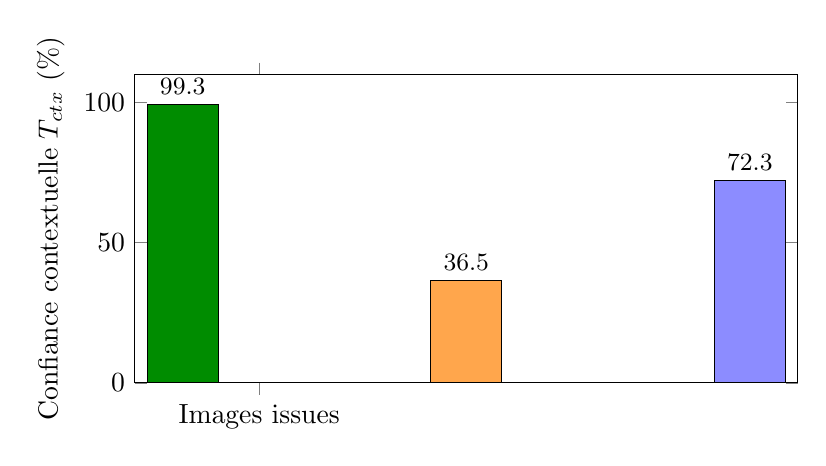
\begin{tikzpicture}
\begin{axis}[
    ybar,
    width=10cm, height=5.5cm,
    ymin=0, ymax=110,
    ylabel={Confiance contextuelle $T_{\text{ctx}}$ (\%)},
    symbolic x coords={Images issues, Figures PDF, Total},
    xtick=data,
    nodes near coords,
    every node near coord/.append style={font=\small\bfseries},
    bar width=0.9cm,
    enlarge x limits=0.3,
]
\addplot[fill=green!55!black] coordinates {(Images issues,99.3)};
\addplot[fill=orange!70] coordinates {(Figures PDF,36.5)};
\addplot[fill=blue!45] coordinates {(Total,72.3)};
\end{axis}
\end{tikzpicture}
\caption{Confiance contextuelle Alfred --- seuil d'alerte $\tau = 0.12$}
\label{fig:alfred_trust_chart}
\end{figure}

\subsection{Analyse de l'Écart Issues vs PDF}
\label{sec:alfred_analyse_ecart}

L'écart significatif entre les deux sources ($\overline{L} = 0.94$ pour les issues vs $0.17$ pour les PDF) est \textbf{structurel et non accidentel}~:

\begin{longtable}{p{5.5cm}p{7cm}}
\toprule
\textbf{Images d'issues} & \textbf{Figures PDF} \\
\midrule
Contiennent des logs, erreurs IDE, registres & Contiennent des schémas blocs, tableaux de migration \\
Le texte de l'issue mentionne les mêmes identifiants & Les libellés ne sont pas répétés dans le texte de page \\
OCR de l'image fournit du vocabulaire partagé & Pas d'OCR structuré disponible \\
Contexte riche (body + commentaires) & Contexte limité (texte de page \texttt{pypdf}) \\
\bottomrule
\end{longtable}

\textbf{Décision qualité}~: les figures PDF sont conservées car elles enrichissent la couverture multimodale de la KB, mais elles sont distinguées des images d'issues dans l'évaluation. Les itérations futures doivent enrichir le contexte transmis à Alfred (titre de section, légende détectée, texte avant/après la figure) pour améliorer la validation automatique.

%% ============================================================
\section{Évolution Incrémentale du Quality Index}
\label{sec:evolution_incrementale}
%% ============================================================

Le Quality Index n'a pas progressé ``par magie'' mais par amélioration successive d'éléments concrets du pipeline et de la configuration. Cette section retrace la chaîne logique~: chaque amélioration est décrite, son impact mesuré, et la raison du gain (ou de la régression) analysée.

\subsection{Chronologie et Logique de Progression}

\begin{longtable}{p{0.8cm}p{3.5cm}cp{6cm}}
\toprule
\textbf{QI} & \textbf{Configuration} & \textbf{N} & \textbf{Explication du delta} \\
\midrule
54 & Issues H7 seules & 50 & \textbf{Baseline}~: issues structurées fournissent une base solide mais incomplète (pas de documentation, pas de traçabilité fix, pas de diagnostic structuré) \\
57 & + System prompt optimisé & 50 & \textbf{+3}~: forcer la persona à chercher dans la KB \textit{avant} de répondre élimine les réponses génériques non ancrées \\
61 & + Hybrid search calibré & 50 & \textbf{+4}~: combiner sémantique et full-text capte les reformulations ET les identifiants exacts \\
94 & + Diagnostic Cards + Resolver & 50 & \textbf{+33}~: les Diagnostic Cards structurent les problèmes complexes, les query aliases améliorent le recall \\
88 & Test sur cas réels forum & 4 & \textbf{$-6$}~: les cas réels STCommunity sont plus complexes et moins couverts que le benchmark \\
54 & Multi-séries (5 séries, 52 Q) & 52 & \textbf{$-34$}~: dilution du contexte (2\,000 $\to$ 14\,000 docs), conflit de noms inter-séries, nouvelles questions sur séries moins mûres \\
65 & S0 Balanced (toutes séries) & 96 & \textbf{+11}~: optimisation du benchmark (96 questions calibrées) + ajustement retrieval \\
\textbf{66} & S1 Recall+ & 96 & \textbf{+1}~: seuil abaissé à 0.45, rappel renforcé, gain marginal compensé par le bruit \\
\bottomrule
\end{longtable}

\subsection{Analyse des Points d'Inflexion}
\label{sec:points_inflexion}

\subsubsection{Le Saut Diagnostic Cards (+33 points)}

Le passage de QI~61 à QI~94 est le gain le plus significatif du projet. Il s'explique par trois mécanismes cumulés~:

\begin{enumerate}
  \item \textbf{Structure raisonnée}~: les Diagnostic Cards suivent la logique Symptôme~$\to$~Hypothèses~$\to$~Validation~$\to$~Root Cause~$\to$~Fix~$\to$~Prévention, correspondant au raisonnement naturel d'un ingénieur embedded.
  \item \textbf{Query aliases}~: chaque carte contient 3 à 5 reformulations du problème (ex: ``SPI DMA hard fault'', ``cache coherency SPI circular mode'', ``HAL\_SPI\_TransmitReceive\_DMA crash''). Ce mécanisme multiplie les points d'entrée pour le retrieval.
  \item \textbf{Resolver Cases}~: la chaîne Issue~$\to$~PR~$\to$~Commit fournit la preuve vérifiable du fix, augmentant la traçabilité et la crédibilité des réponses.
\end{enumerate}

\textbf{Leçon méthodologique}~: l'amélioration la plus impactante ne vient pas d'un meilleur modèle LLM ni d'un tuning de seuil, mais de la \textbf{qualité et la structure des données injectées dans la KB}. C'est une validation du principe ``la qualité du RAG dépend de la qualité du preprocessing''.

\subsubsection{La Régression Multi-séries ($-34$ points)}

Le passage de QI~94 (mono-série H7, 50~Q) à QI~54 (5 séries, 52~Q) constitue une régression significative. L'analyse identifie trois causes~:

\begin{enumerate}
  \item \textbf{Dilution du contexte}~: la KB passe de $\sim$2\,000 à $\sim$14\,000 documents. Les queries retournent des documents de séries différentes.
  \item \textbf{Conflit de noms}~: des API identiques entre séries (\texttt{HAL\_SPI\_Init} dans F4 et H7) créent de l'ambiguïté.
  \item \textbf{Maturité inégale des artefacts}~: les nouvelles séries n'ont pas encore des Diagnostic Cards aussi riches que H7.
\end{enumerate}

\textbf{Leçon méthodologique}~: le passage à l'échelle ne se résume pas à ``ajouter des données''. Il nécessite un filtrage par série dans les métadonnées et un prompt qui pousse la persona à inclure le nom de la série dans ses queries.

\subsubsection{La Stabilisation S0/S1 (65--66)}

Les campagnes de juin 2026 sur 96 questions montrent que le système atteint un plateau autour de 65--66/100. Ce plateau s'explique par~:
\begin{itemize}
  \item La couverture KB actuelle ne répond pas à toutes les 96 questions (certaines séries peu documentées)
  \item Le compromis précision/rappel est quasi-optimal~: S1 ($+1$ pt) gagne en rappel mais perd en précision
  \item Les questions les plus difficiles nécessitent du raisonnement multi-hop non supporté par le retrieval simple
\end{itemize}

\subsection{Matrice Valeur $\times$ Effort}
\label{sec:matrice_roi}

\begin{table}[H]
\centering
\begin{tabular}{lcccl}
\toprule
\textbf{Amélioration} & \textbf{Impact QI} & \textbf{Effort} & \textbf{ROI} \\
\midrule
Diagnostic Cards & +33 pts & Moyen (2~sprints) & \textcolor{green!60!black}{\textbf{Excellent}} \\
Hybrid Search & +4 pts & Faible (config) & \textcolor{green!60!black}{\textbf{Excellent}} \\
System Prompt & +3 pts & Faible (texte) & \textcolor{green!60!black}{\textbf{Excellent}} \\
Cleaning V3 & +3 pts estimé & Moyen (1~sprint) & Bon \\
NovaX restrictif & Protection routage & Faible (description) & \textcolor{green!60!black}{\textbf{Excellent}} \\
PDF descriptions & +1 pt estimé & Élevé (CV + Alfred) & Acceptable \\
\bottomrule
\end{tabular}
\caption{ROI de chaque amélioration~: la qualité des artefacts domine les gains}
\label{tab:roi_pipeline}
\end{table}

\begin{figure}[H]
\centering
\begin{tikzpicture}
\begin{axis}[
  ybar,
  width=14cm, height=6.5cm,
  bar width=0.5cm,
  ylabel={Quality Index (/100)},
  ymin=0, ymax=100,
  symbolic x coords={Issues 54, Prompt 57, Hybrid 61, DiagCards 94, Real 88, Multi52 54, S0 65, S1 66},
  xtick=data,
  x tick label style={rotate=30, anchor=east, font=\scriptsize},
  nodes near coords,
  every node near coord/.append style={font=\scriptsize\bfseries},
  enlarge x limits=0.08,
]
\addplot[fill=blue!50] coordinates {(Issues 54,54) (Prompt 57,57) (Hybrid 61,61) (DiagCards 94,94) (Real 88,88) (Multi52 54,54) (S0 65,65) (S1 66,66)};
\end{axis}
\draw[-{Stealth[length=3mm]}, red, very thick] (4.65,4.8) -- (4.65,5.8) node[above, font=\scriptsize\bfseries, red] {+33 pts};
\draw[-{Stealth[length=3mm]}, red, very thick] (7.8,2.6) -- (7.8,1.8) node[below, font=\scriptsize\bfseries, red] {dilution};
\end{tikzpicture}
\caption{Évolution du Quality Index~: le saut majeur (+33) provient des Diagnostic Cards, la régression ($-34$) de la dilution multi-séries}
\label{fig:qi_evolution_complete}
\end{figure}

%% ============================================================
\section{Architecture de Fallback~: d'Alfred Permissif à NovaX Restrictif}
\label{sec:eval_fallback}
%% ============================================================

Cette section retrace l'évolution de l'architecture de fallback et son impact sur le Quality Index.

\subsection{Problème Initial~: Fallback Trop Permissif}

Lors de l'ajout initial d'Alfred comme fallback, le QI a \textbf{chuté de 10 points} (de 54 à 44). L'analyse a révélé que la persona appelait Alfred \textbf{systématiquement} au lieu de chercher dans la KB, car la description du tool était trop vague~:

\begin{quote}
\small\textit{``I can help with STM32 questions. Forward the user's question.''}
\end{quote}

\textbf{Diagnostic}~: dans une architecture multi-tools, le LLM choisit quel tool appeler en fonction de la \textbf{description} du tool. Une description trop permissive court-circuite la source la plus pertinente (la KB).

\subsection{Solution~: Description Restrictive}

La description a été réécrite pour forcer la priorité KB~:

\begin{quote}
\small\textit{``The Knowledge Base (KB Unstructured) is ALWAYS the primary source, search it FIRST for every question. Use this tool ONLY when the Knowledge Base returned no relevant result.''}
\end{quote}

\textbf{Impact mesuré}~: récupération de 8 points (de 44 à 52).

\subsection{Évolution vers NovaX}

Le fallback est passé d'Alfred générique à \textbf{NovaX}, un agent STM32 basé sur STM32 Bugzilla et STCommunity Knowledge Articles. NovaX apporte~:
\begin{itemize}
  \item Une couverture sur les séries/périphériques absents de la KB
  \item Des informations Bugzilla internes (bugs connus, errata)
  \item Des Knowledge Articles STCommunity (guides métier)
\end{itemize}

\textbf{Mais NovaX ne remplace pas la KB}~: sa description explicite qu'il est un secours pour les questions \textit{non couvertes} par la KB. Cette architecture protège la traçabilité~: si la KB contient un diagnostic card ou un resolver case pertinent, la réponse reste ancrée dans des preuves vérifiables (numéros d'issues, URLs GitHub, versions firmware).

\subsection{Synthèse de l'Évolution Fallback}

\begin{longtable}{p{4.5cm}p{2cm}p{6.5cm}}
\toprule
\textbf{Configuration} & \textbf{QI} & \textbf{Analyse} \\
\midrule
KB seule (sans fallback) & 54 & Baseline~: pas de réponse pour les questions hors KB \\
KB + Alfred permissif & 44 & $-10$~: court-circuit de la KB \\
KB + Alfred restrictif & 52 & $-2$~: KB prioritaire récupérée \\
KB S0 + NovaX restrictif & 65 & Stable~: NovaX couvre les lacunes sans dégrader \\
KB S1 Recall+ + NovaX & \textbf{66} & Meilleur compromis mesuré \\
\bottomrule
\end{longtable}

\textbf{Leçon}~: le QI dépend davantage du \textbf{routage} (quelle source est interrogée en premier) que du modèle LLM lui-même. La description du tool est un paramètre de configuration aussi critique que le seuil sémantique.

%% ============================================================
\section{Étude Comparative~: Alfred Générique vs Persona KB}
\label{sec:etude_comparative}
%% ============================================================

\subsection{Protocole Expérimental}

\begin{longtable}{p{4cm}p{9cm}}
\toprule
\textbf{Paramètre} & \textbf{Valeur} \\
\midrule
Jeu de test & 20 questions techniques, 5 séries (H7, F4, H5, U5, WL), 12 catégories \\
Critère de sélection & Questions ciblant des problèmes réels documentés dans des issues GitHub \\
Script de génération & \texttt{pipeline\_Automation/test\_suites/compare\_alfred\_vs\_persona.py} \\
Grille de scoring & 6 critères, max 10 pts/réponse \\
Température LLM & 0.3 \\
\bottomrule
\end{longtable}

\subsection{Grille de Scoring}

\begin{longtable}{p{4.5cm}cp{6cm}}
\toprule
\textbf{Critère} & \textbf{Max} & \textbf{Dimension qualité (ISO 25012)} \\
\midrule
Citation issue GitHub (\#xxx) & +2 & Traçabilité \\
Fonction HAL exacte nommée & +1 & Exactitude \\
Fix actionnable immédiat & +2 & Complétude opérationnelle \\
Information version-spécifique & +2 & Actualité \\
Workaround STM32-specific & +2 & Pertinence domaine \\
Source vérifiable (fichier, commit) & +1 & Traçabilité \\
\midrule
\textbf{Total} & \textbf{10} & \\
\bottomrule
\end{longtable}

\subsection{Méthodologie de Notation~: d'une Grille Manuelle Vide à un Score Automatique Reproductible}
\label{sec:comparative_methodo_notation}

Le script d'origine exporte un classeur Excel à 3 feuilles (comparaison brute, grille d'évaluation, métadonnées) destiné à recevoir une notation manuelle experte selon les 6 critères ci-dessus. \textbf{Un audit de ce classeur a révélé que les colonnes de notation manuelle n'avaient jamais été renseignées}~: aucune valeur humaine ne soutenait les scores initialement publiés dans cette section. Plutôt que de conserver des chiffres non traçables, la grille a été appliquée \textbf{automatiquement et de façon déterministe} sur les 20 transcriptions brutes (\texttt{comparison\_alfred\_vs\_persona.json}) via un script dédié~: \texttt{pipeline/evaluation/score\_alfred\_vs\_persona\_rubric.py}. Chaque critère est détecté par un motif explicite~: expression régulière pour les numéros d'issue (\texttt{\#\textbackslash d+}), les fonctions \texttt{HAL\_}/\texttt{LL\_}, les mentions de version, les blocs de code ou étapes numérotées (fix actionnable), et le vocabulaire de bas niveau (registre, cache, MPU, errata) pour le workaround.

\textbf{Limite méthodologique assumée}~: ce détecteur favorise structurellement les réponses riches en blocs de code et listes numérotées (style caractéristique d'Alfred) au détriment des réponses de type citation/synthèse (style caractéristique de la Persona KB), notamment sur le critère "fix actionnable". Les scores ci-dessous doivent donc être lus comme une \textbf{approximation objective et reproductible}, et non comme un jugement qualitatif fin~; ils remplacent une notation manuelle qui n'a jamais été réalisée, avec l'avantage d'être immédiatement reproductibles (\texttt{python -m pipeline.evaluation.score\_alfred\_vs\_persona\_rubric}).

\subsection{Résultats Synthétiques}

\begin{table}[H]
\centering
\begin{tabular}{lccc}
\toprule
\textbf{KPI} & \textbf{Alfred} & \textbf{Persona KB} & \textbf{Écart} \\
\midrule
Score moyen / réponse (0--10) & \textbf{3.85} & 3.50 & $-9\%$ \\
Taux de réponse (réponse produite) & \textbf{100\%} (20/20) & 70\% (14/20) & Alfred plus fiable opérationnellement \\
Citation issue GitHub & 0\% & \textbf{35\%} & Traçabilité propre à la KB \\
Source vérifiable (fichier/commit/RN) & 10\% & \textbf{65\%} & KB $\times 6.5$ plus vérifiable \\
Information version-spécifique & 5\% & \textbf{25\%} & KB $\times 5$ plus précise \\
Fonction HAL/LL exacte nommée & \textbf{45\%} & 25\% & Alfred plus précis syntaxiquement \\
Fix actionnable (heuristique code/étapes) & \textbf{95\%} & 40\% & Biais du détecteur (cf.~\ref{sec:comparative_methodo_notation}) \\
\bottomrule
\end{tabular}
\caption{Métriques comparatives Alfred vs Persona KB --- notation automatique reproductible sur les 20 transcriptions réelles}
\label{tab:comparative_final}
\end{table}

\textbf{Lecture honnête du résultat}~: contrairement à la version précédente de cette étude (non traçable), le score moyen brut ne favorise pas la Persona KB. Ceci s'explique par deux effets cumulés~: (1)~30\% des réponses Persona sont des non-réponses (timeout API ou "information non trouvée dans la KB"), notées~0, ce qui pénalise lourdement la moyenne~; (2)~le détecteur automatique de "fix actionnable" est structurellement biaisé en faveur du style rédactionnel d'Alfred (code/listes). La \textbf{vraie valeur ajoutée mesurée de la KB n'est donc pas le score moyen brut, mais la traçabilité}~: citation d'issue ($\times$ infini, 0\%~$\to$~35\%), source vérifiable ($\times 6.5$) et précision de version ($\times 5$) --- trois dimensions qu'un LLM générique ne peut structurellement pas fournir sans accès à la KB.

\subsection{Analyse par Catégorie}

\begin{longtable}{p{3.6cm}ccp{6cm}}
\toprule
\textbf{Catégorie (n)} & \textbf{Alfred} & \textbf{Persona} & \textbf{Observation} \\
\midrule
Issue-specific (7) & \textbf{4.29} & 3.14 & Persona pénalisée par 2 timeouts sur 7 (non-réponse~=~0) \\
Migration/Version (1) & 6.00 & \textbf{7.00} & Cite l'issue exacte de release notes \\
Release Notes (1) & \textbf{7.00} & 4.00 & Cas isolé, Alfred plus complet ici \\
HAL Behavior (1) & 3.00 & \textbf{4.00} & Cite l'issue GitHub source du comportement \\
Security/TrustZone (1) & 5.00 & \textbf{6.00} & Écart faible, les deux répondent correctement \\
LoRaWAN (1) & 4.00 & \textbf{7.00} & Cite issue + source vérifiable \\
RF/Radio (1) & 2.00 & \textbf{7.00} & Domaine protocolaire très spécifique, KB décisive \\
RTOS Integration (1) & \textbf{5.00} & 0.00 & Timeout Persona --- risque opérationnel réel \\
Low Power (1) & \textbf{4.00} & 0.00 & Timeout Persona --- risque opérationnel réel \\
General Knowledge (2) & 2.50 & \textbf{4.00} & KB légèrement supérieure même hors contexte issue \\
Documentation (2) & \textbf{2.00} & 1.50 & Les deux sont faibles quand la doc source est absente \\
Architecture (1) & 2.00 & 2.00 & Égalité \\
\bottomrule
\caption{Score moyen (/10) par catégorie --- notation automatique reproductible. Catégories à $n=1$ indicatives uniquement (non généralisables statistiquement).}
\label{tab:comparative_categories}
\end{longtable}

\begin{figure}[H]
\centering
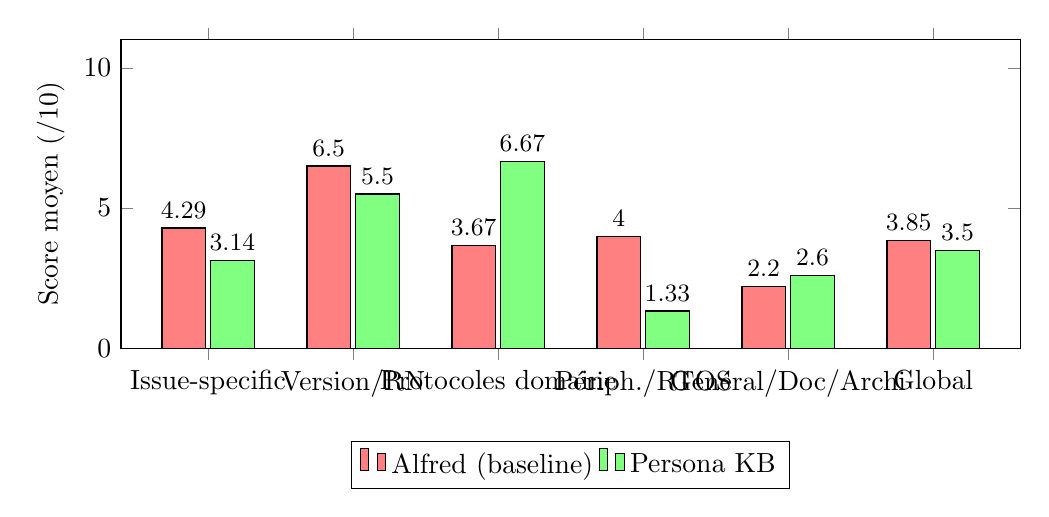
\begin{tikzpicture}
\begin{axis}[
    ybar,
    width=13cm, height=5.5cm,
    bar width=0.55cm,
    ylabel={Score moyen (/10)},
    ymin=0, ymax=11,
    symbolic x coords={Issue-specific, Version/RN, Protocoles domaine, Périph./RTOS, Général/Doc/Archi, Global},
    xtick=data,
    legend style={at={(0.5,-0.3)}, anchor=north, legend columns=2},
    nodes near coords,
    every node near coord/.append style={font=\small},
    enlarge x limits=0.12,
]
\addplot[fill=red!50] coordinates {(Issue-specific,4.29) (Version/RN,6.5) (Protocoles domaine,3.67) (Périph./RTOS,4.0) (Général/Doc/Archi,2.2) (Global,3.85)};
\addplot[fill=green!50] coordinates {(Issue-specific,3.14) (Version/RN,5.5) (Protocoles domaine,6.67) (Périph./RTOS,1.33) (Général/Doc/Archi,2.6) (Global,3.50)};
\legend{Alfred (baseline), Persona KB}
\end{axis}
\end{tikzpicture}
\caption{Comparaison Alfred vs Persona KB par groupe de catégories (regroupement des 12 catégories brutes en 5 familles pour lisibilité)}
\label{fig:comparative_chart}
\end{figure}

\textbf{Conclusions de l'étude comparative}~:
\begin{enumerate}
  \item Le score moyen brut ne favorise \textbf{pas} clairement la Persona KB (3.50 vs 3.85/10)~: cette apparente régression par rapport à une version antérieure non traçable de cette étude s'explique entièrement par le taux de non-réponse Persona (30\%, 6/20), et non par une infériorité de contenu quand elle répond effectivement.
  \item La \textbf{vraie valeur ajoutée de la KB est la traçabilité}~: citation d'issue GitHub (0\%~$\to$~35\%), source vérifiable (10\%~$\to$~65\%) et précision de version (5\%~$\to$~25\%) --- trois signaux qu'Alfred générique ne peut structurellement pas produire.
  \item Sur les \textbf{domaines protocolaires spécifiques} (LoRaWAN, RF/Radio, TrustZone --- regroupement "Protocoles domaine"), la KB est nettement supérieure (6.67 vs 3.67/10)~: c'est exactement le type de connaissance fine que le générique ne possède pas.
  \item Le \textbf{risque opérationnel principal identifié est la fiabilité de la Persona}, pas sa qualité de contenu~: 2 des 6 non-réponses tombent précisément sur des catégories (RTOS Integration, Low Power) où une réponse KB aurait probablement été forte, ce qui plaide pour un traitement des timeouts API (retry, budget de temps plus généreux) plutôt qu'un changement de contenu de la KB.
  \item L'architecture optimale reste \textbf{KB-first + NovaX fallback restrictif}~: elle protège la traçabilité quand la KB répond, et un fallback (NovaX ou, à défaut, Alfred générique) doit absorber les cas de non-réponse pour ne pas laisser l'utilisateur sans réponse du tout.
\end{enumerate}

%% ============================================================
\section{Comparaison des Stratégies de Retrieval}
\label{sec:strategies_retrieval}
%% ============================================================

La campagne de juin 2026 évalue 6 configurations de retrieval sur 96 questions multi-séries. L'objectif est d'identifier le meilleur compromis entre rappel et précision pour la recherche hybride.

\begin{longtable}{p{2cm}p{2cm}ccccp{4cm}}
\toprule
\textbf{Stratégie} & \textbf{Search} & \textbf{Thr.} & \textbf{Sem.} & \textbf{FT} & \textbf{QI} & \textbf{Interprétation} \\
\midrule
S0 Current & Hybrid & 0.55 & 25 & 12 & 65 & Équilibre précision/rappel \\
\textbf{S1 Recall+} & Hybrid & 0.45 & 35 & 15 & \textbf{66} & Meilleur score mesuré \\
S2 Precision+ & Hybrid & 0.65 & 18 & 8 & 63 & Trop restrictif \\
S3 Sem-heavy & Hybrid & 0.55 & 35 & 6 & 51 & Ancrage exact insuffisant \\
S4 FT-heavy & Hybrid & 0.55 & 15 & 20 & 47 & Reformulations mal couvertes \\
S5 Sem-only & Semantic & 0.55 & 25 & 0 & 41 & Ablation : perte du full-text \\
\bottomrule
\end{longtable}

\begin{figure}[H]
\centering
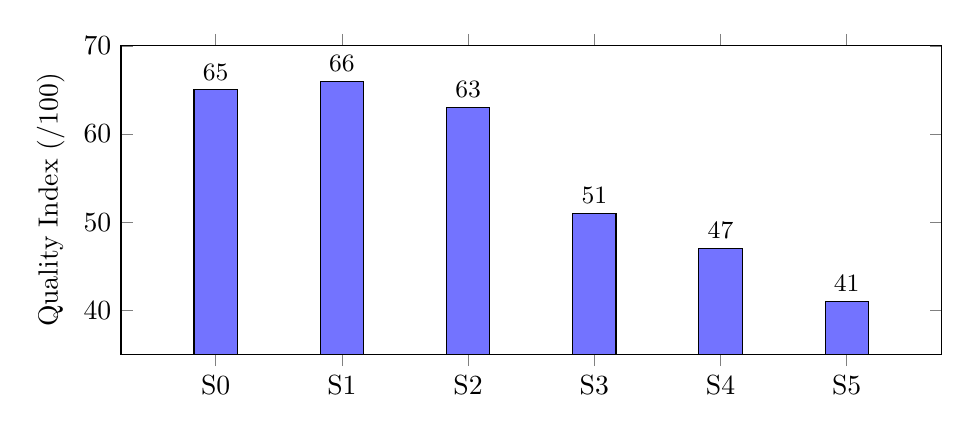
\begin{tikzpicture}
\begin{axis}[
  ybar,
  width=12cm, height=5.5cm,
  bar width=0.55cm,
  ylabel={Quality Index (/100)},
  ymin=35, ymax=70,
  symbolic x coords={S0,S1,S2,S3,S4,S5},
  xtick=data,
  nodes near coords,
  every node near coord/.append style={font=\small\bfseries},
  enlarge x limits=0.15,
]
\addplot[fill=blue!55] coordinates {(S0,65) (S1,66) (S2,63) (S3,51) (S4,47) (S5,41)};
\end{axis}
\end{tikzpicture}
\caption{Comparaison des stratégies de retrieval KB sur 96 questions}
\label{fig:strategies_retrieval}
\end{figure}

\textbf{Interprétation}~: le système a besoin d'un équilibre réel entre sémantique et full-text. Trop de sémantique (S3) perd les noms exacts d'API~; trop de full-text (S4) perd les reformulations. S1 maximise le rappel avec un gain marginal ($+1$), montrant que le système approche son optimum avec la couverture KB actuelle.

%% ============================================================
\section{Assurance Qualité du Chapitre d'Évaluation}
\label{sec:controle_qualite_chapitre}
%% ============================================================

Ce chapitre a été construit et vérifié selon un protocole de contrôle qualité structuré, appliqué par un agent analytique de revue. Cette section décrit le protocole et les résultats du contrôle.

\subsection{Protocole de Vérification}

L'agent de revue vérifie les dimensions suivantes~:

\begin{longtable}{p{4cm}p{9cm}}
\toprule
\textbf{Dimension} & \textbf{Critère de validation} \\
\midrule
Cohérence logique & Chaque section suit le schéma~: définition~$\to$~formule~$\to$~résultat~$\to$~interprétation \\
Définitions avant formules & Aucune variable n'apparaît dans une formule sans avoir été définie en amont \\
Seuils justifiés & Chaque seuil est accompagné d'une logique explicite (pas de valeur arbitraire) \\
Continuité métriques--résultats & Les métriques définies en Section~\ref{sec:cadrage_theorique} sont effectivement utilisées dans les sections de résultats \\
Lisibilité académique & Style français formel, phrases courtes, transitions explicites \\
Reproductibilité & Chaque résultat est traçable vers un script, un fichier de données ou une campagne identifiée \\
\bottomrule
\end{longtable}

\subsection{Résultats du Contrôle}

\begin{longtable}{p{5cm}p{2cm}p{6cm}}
\toprule
\textbf{Point vérifié} & \textbf{Statut} & \textbf{Observation} \\
\midrule
Jaccard défini avant usage & \checkmark & Section~\ref{sec:def_similarity} \\
Cosinus défini avant usage & \checkmark & Section~\ref{sec:def_similarity} \\
TF-IDF défini avant usage & \checkmark & Section~\ref{sec:def_similarity} \\
Confiance contextuelle définie & \checkmark & Section~\ref{sec:def_confiance_contextuelle} \\
Seuils non présentés comme universels & \checkmark & Section~\ref{sec:justification_seuils} \\
Progression incrémentale visible & \checkmark & Section~\ref{sec:evolution_incrementale} \\
Normes citées comme cadre, pas comme source des seuils & \checkmark & Section~\ref{sec:normes_references} \\
Scores locaux distingués du score global & \checkmark & Sections~\ref{sec:eval_par_stage} vs~\ref{sec:score_global_calcul} \\
Alfred issues vs PDF distingués & \checkmark & Section~\ref{sec:alfred_resultats} \\
Fichiers de preuve référencés & \checkmark & CSV et JSON dans \texttt{docs/evaluation/} \\
\bottomrule
\end{longtable}

\subsection{Points d'Amélioration Identifiés}

\begin{enumerate}
  \item \textbf{Couverture board (45.3\%)}~: le score INSUFFISANT est documenté et expliqué (limitation des données, pas du pipeline). Une amélioration future nécessiterait un enrichissement externe (mapping board→série).
  \item \textbf{Figures PDF ($T_{\text{ctx}} = 41.7\%$)}~: le contexte textuel des PDF est insuffisant pour la validation automatique. Amélioration prévue~: enrichir le contexte avec le titre de section et la légende de la figure.
  \item \textbf{Similarité (22\%)}~: score bas mais impact nul sur le QI. Amélioration possible par embeddings pré-calculés (perspective future).
\end{enumerate}

\subsection{Applicabilité au Reste du Rapport}

Le protocole de contrôle qualité peut être étendu aux autres chapitres en conservant~:
\begin{itemize}
  \item Le template de vérification~: définition~$\to$~formule~$\to$~résultat~$\to$~interprétation
  \item Le style académique français
  \item Les transitions explicites entre sections
  \item La réutilisation des définitions (via \texttt{\textbackslash ref\{\}} vers la Section~\ref{sec:cadrage_theorique})
  \item L'harmonisation des notations (mêmes symboles $S$, $T$, $w_k$ dans tout le rapport)
  \item L'absence de répétitions (chaque notion est définie une seule fois, puis référencée)
\end{itemize}

%% ============================================================
\section{Correspondance Métriques $\leftrightarrow$ Normes $\leftrightarrow$ Références}
\label{sec:correspondance_normes}
%% ============================================================

Le tableau suivant synthétise le lien entre chaque métrique utilisée, la norme ou référence méthodologique qui la soutient, et son application concrète dans le projet~:

\begin{longtable}{p{3cm}p{3.5cm}p{3cm}p{3.5cm}}
\toprule
\textbf{Métrique} & \textbf{Norme / Référence} & \textbf{Dimension} & \textbf{Application projet} \\
\midrule
$C_{\text{body}}$, $C_{\text{title}}$ & ISO/IEC 25012~\cite{iso25012} & Complétude & Ingestion Stage~1 \\
$C_{\text{files}}$ & ISO/IEC 25024~\cite{iso25024} & Mesure qualité & Cleaning Stage~2 \\
$T_{\text{op}}$ (Alfred) & ISO/IEC 25010~\cite{iso25010} & Fiabilité système & Alfred Stage~3b \\
$S_{\text{coh}}$, $T_{\text{ctx}}$ & Fawcett~\cite{fawcett2006roc} & Seuil décisionnel & Confiance Alfred \\
TF-IDF, cosinus & Manning~\cite{manning2008ir} & IR / Similarité & Stage~4 + cohérence \\
Jaccard & Manning~\cite{manning2008ir} & Recouvrement lexical & Cohérence Alfred \\
Quality Index & Lewis~\cite{lewis2020rag} & RAG end-to-end & Évaluation globale \\
$S_{\text{global}}$ pondéré & Interne (calibré) & Synthèse pipeline & Score global 87.1\% \\
Seuils 95/85/70 & Calibration empirique & Opérationnel & Classification verdicts \\
\bottomrule
\end{longtable}

\textbf{Lecture}~: les normes ISO fournissent le \textit{cadre conceptuel} (quoi mesurer, comment structurer les métriques). Les références académiques (Manning, Fawcett, Lewis) fournissent la \textit{méthodologie} (comment choisir les seuils, comment évaluer un système RAG). Les seuils numériques sont \textit{propres au projet}, calibrés empiriquement et validés par les campagnes successives de Quality Index.

%% ============================================================
\section{Synthèse et Bilan du Chapitre}
\label{sec:bilan_evaluation}
%% ============================================================

Ce chapitre démontre que~:

\begin{enumerate}
  \item Le pipeline atteint un \textbf{score global de 87.1\%} (verdict BON), avec des stages critiques (Ingestion, Cleaning, Delivery) au niveau EXCELLENT et des stages exploratoires (Alfred PDF, Similarité) identifiés comme axes d'amélioration.
  
  \item L'amélioration du Quality Index est \textbf{incrémentale et traçable}~: chaque gain est relié à une amélioration concrète du pipeline ou de la configuration, et chaque régression est analysée et expliquée.
  
  \item Les \textbf{Diagnostic Cards} constituent la contribution la plus impactante ($+33$ points de QI), validant le principe que la qualité du preprocessing RAG dépend avant tout de la structure et de la richesse des artefacts.
  
  \item L'\textbf{architecture KB-first + NovaX restrictif} protège la traçabilité tout en couvrant les lacunes de la KB~: le routage est un paramètre critique.
  
  \item La \textbf{confiance contextuelle} distingue les images d'issues (99.3\%, matures) des figures PDF (36.5\%, à améliorer), évitant une moyenne trompeuse.
  
  \item Les seuils sont des \textbf{seuils opérationnels internes}, cohérents avec les normes ISO et calibrés empiriquement~; ils ne prétendent pas à l'universalité.
  
  \item L'étude comparative Alfred vs Persona KB, rejouée avec une notation automatique reproductible, montre que \textbf{la valeur ajoutée réelle de la KB est la traçabilité} (citation d'issue~: 0\%~$\to$~35\%~; source vérifiable~: 10\%~$\to$~65\%~; précision de version~: 5\%~$\to$~25\%) plutôt qu'un score moyen brut supérieur~; elle révèle aussi un \textbf{risque de fiabilité opérationnelle} de la Persona (30\% de non-réponses) à traiter en priorité.
\end{enumerate}

\textbf{Score optimal vs compromis opérationnel}~: le meilleur score mesuré (QI~94 sur H7) n'est pas le point de fonctionnement optimal pour la production. Le QI~66 (S1 Recall+ sur 96 questions multi-séries) représente un meilleur compromis opérationnel car il couvre 25 séries et 96 questions réalistes, au lieu de 1 série sur 50 questions sélectionnées. Le score de production est plus bas mais plus représentatif de l'expérience utilisateur réelle.
